% UCL Thesis LaTeX Template
% 
% This is a template/skeleton for PhD/MPhil/MRes theses.
%
% It uses a rather split-up file structure because this tends to
%  work well for large, complex documents.
% We suggest using one file per chapter, but you may wish to use more
%  or fewer separate files than that.
% We've also separated out various bits of configuration into their
%  own files, to keep everything neat.
% Note that the \input command just streams in whatever file you give
%  it, while the \include command adds a page break, and does some
%  extra organisation to make compilation faster. Note that you can't
%  use \include inside an \include-d file.
% We suggest using \input for settings and configuration files that
%  you always want to use, and \include for each section of content.
% If you do that, it also means you can use the \includeonly statement
%  to only compile up the section you're currently interested in.
% You might also want to put figures into their own files to be \input.

% For more information on \input and \include, see:
%  http://tex.stackexchange.com/questions/246/when-should-i-use-input-vs-include


% Formatting rules for theses are here: 
%  http://www.ucl.ac.uk/current-students/research_degrees/thesis_formatting
% Binding and submitting guidelines are here:
%  http://www.ucl.ac.uk/current-students/research_degrees/thesis_binding_submission

% This package goes first and foremost, because it checks all 
%  your syntax for mistakes and some old-fashioned LaTeX commands.
% Note that normally you should load your documentclass before 
%  packages, because some packages change behaviour based on
%  your document settings.
% Also, for those confused by the RequirePackage here vs usepackage
%  elsewhere, usepackage cannot be used before the documentclass
%  command, while RequirePackage can. That's the only functional
%  difference.
\RequirePackage[l2tabu, orthodox]{nag}


% ------ Main document class specification ------
% The draft option here prevents images being inserted,
%  and adds chunky black bars to boxes that are exceeding 
%  the page width (to show that they are).
% The oneside option can optionally be replaced by twoside if
%  you intend to print double-sided. Note that this is
%  *specifically permitted* by the UCL thesis formatting
%  guidelines.
%
% Valid options in terms of type are:
%  phd
%  mres
%  mphil
%\documentclass[12pt,phd,draft,a4paper,oneside]{ucl_thesis}
\documentclass[12pt,phd,a4paper,oneside]{ucl_thesis}


% Package configuration:
%  LaTeX uses "packages" to add extra commands and features.
%  There are quite a few useful ones, so we've put them in a 
%   separate file.
% -------- Packages --------

% This package just gives you a quick way to dump in some sample text.
% You can remove it -- it's just here for the examples.
\usepackage{blindtext}

% This package means empty pages (pages with no text) won't get stuff
%  like chapter names at the top of the page. It's mostly cosmetic.
\usepackage{emptypage}

% The graphicx package adds the \includegraphics command,
%  which is your basic command for adding a picture.
\usepackage{graphicx}

% This command is provided by the graphicx package, and 
%  controls the default dpi resolution of images you use.
%  72 is the default, but 300 is more normal, and 600 is
%  as good as you can expect to be able to get on normal paper.
\pdfimageresolution=300


% The float package improves LaTeX's handling of floats,
%  and also adds the option to *force* LaTeX to put the float
%  HERE, with the [H] option to the float environment.
\usepackage{float}

% The amsmath package enhances the various ways of including
%  maths, including adding the align environment for aligned
%  equations.
\usepackage{amsmath}

% Use these two packages together -- they define symbols
%  for e.g. units that you can use in both text and math mode.
\usepackage{gensymb}
\usepackage{textcomp}
% You may also want the units package for making little
%  fractions for unit specifications.
%\usepackage{units}


% The setspace package lets you use 1.5-sized or double line spacing.
\usepackage{setspace}
\setstretch{1.5}

% That just does body text -- if you want to expand *everything*,
%  including footnotes and tables, use this instead:
%\renewcommand{\baselinestretch}{1.5}


% PGFPlots is either a really clunky or really good way to add graphs
%  into your document, depending on your point of view.
% There's waaaaay too much information on using this to cover here,
%  so, you might want to start here:
%   http://pgfplots.sourceforge.net/
%  or here:
%   http://pgfplots.sourceforge.net/pgfplots.pdf
%\usepackage{pgfplots}
%\pgfplotsset{compat=1.3} % <- this fixed axis labels in the version I was using

% PGFPlotsTable can help you make tables a little more easily than
%  usual in LaTeX.
% If you're going to have to paste data in a lot, I'd suggest using it.
%  You might want to start with the manual, here:
%  http://pgfplots.sourceforge.net/pgfplotstable.pdf
%\usepackage{pgfplotstable}

% These settings are also recommended for using with pgfplotstable.
%\pgfplotstableset{
%	% these columns/<colname>/.style={<options>} things define a style
%	% which applies to <colname> only.
%	empty cells with={--}, % replace empty cells with '--'
%	every head row/.style={before row=\toprule,after row=\midrule},
%	every last row/.style={after row=\bottomrule}
%}


% The mhchem package provides chemistry formula typesetting commands
%  e.g. \ce{H2O}
%\usepackage[version=3]{mhchem}

% And the chemfig package gives a weird command for adding Lewis 
%  diagrams, for e.g. organic molecules
%\usepackage{chemfig}

% The linenumbers command from the lineno package adds line numbers
%  alongside your text that can be useful for discussing edits 
%  in drafts.
% Remove or comment out the command for proper versions.
%\usepackage[modulo]{lineno}
% \linenumbers 


% Alternatively, you can use the ifdraft package to let you add
%  commands that will only be used in draft versions
%\usepackage{ifdraft}

% For example, the following adds a watermark if the draft mode is on.
%\ifdraft{
%  \usepackage{draftwatermark}
%  \SetWatermarkText{\shortstack{\textsc{Draft Mode}\\ \strut \\ \strut \\ \strut}}
%  \SetWatermarkScale{0.5}
%  \SetWatermarkAngle{90}
%}


% The multirow package adds the option to make cells span 
%  rows in tables.
\usepackage{multirow}


% Subfig allows you to create figures within figures, to, for example,
%  make a single figure with 4 individually labeled and referenceable
%  sub-figures.
% It's quite fiddly to use, so check the documentation.
%\usepackage{subfig}

% The natbib package allows book-type citations commonly used in
%  longer works, and less commonly in science articles (IME).
% e.g. (Saucer et al., 1993) rather than [1]
% More details are here: http://merkel.zoneo.net/Latex/natbib.php
%\usepackage{natbib}

% The bibentry package (along with the \nobibliography* command)
%  allows putting full reference lines inline.
%  See: 
%   http://tex.stackexchange.com/questions/2905/how-can-i-list-references-from-bibtex-file-in-line-with-commentary
%\usepackage{bibentry} 
\usepackage[backend=bibtex]{biblatex}
        \addbibresource{export}
% The isorot package allows you to put things sideways 
%  (or indeed, at any angle) on a page.
% This can be useful for wide graphs or other figures.
%\usepackage{isorot}

% The caption package adds more options for caption formatting.
% This set-up makes hanging labels, makes the caption text smaller
%  than the body text, and makes the label bold.
% Highly recommended.
\usepackage[format=hang,font=small,labelfont=bf]{caption}

% If you're getting into defining your own commands, you might want
%  to check out the etoolbox package -- it defines a few commands
%  that can make it easier to make commands robust.
\usepackage{etoolbox}

\usepackage{color}
\usepackage{xcolor}
\usepackage{standalone}
\usepackage{tikz}
    \usetikzlibrary{positioning, shapes}
    \tikzset{main node/.style={circle,draw,minimum size=1cm,inner sep=0pt},
            param node/.style={circle,,draw,minimum size=1cm,inner sep=0pt},
            dec node/.style={draw,minimum size=1cm,inner sep=0pt}}

\usepackage{ulem}
\usepackage{cancel}

%plotting sub figures
\usepackage{adjustbox}
\usepackage{subfig}
\usepackage{booktabs} %not sure what this does but it is something to do with getting tables in sub figures
%Highlight package
\usepackage{soul}
\usepackage{placeins}
\usepackage{lscape}
\usepackage{longtable}

\usepackage [english]{babel}
\usepackage [autostyle, english = american]{csquotes}
\MakeOuterQuote{"}






% Sets up links within your document, for e.g. contents page entries
%  and references, and also PDF metadata.
% You should edit this!
%%
%% This file uses the hyperref package to make your thesis have metadata embedded in the PDF, 
%%  and also adds links to be able to click on references and contents page entries to go to 
%%  the pages.
%%

% Some hacks are necessary to make bibentry and hyperref play nicely.
% See: http://tex.stackexchange.com/questions/65348/clash-between-bibentry-and-hyperref-with-bibstyle-elsart-harv
\usepackage{bibentry}
\makeatletter\let\saved@bibitem\@bibitem\makeatother
\usepackage[pdftex,hidelinks]{hyperref}
\hypersetup{
    colorlinks=true,
    linkcolor=black,
    filecolor=black,      
    urlcolor=blue,
}
\makeatletter\let\@bibitem\saved@bibitem\makeatother
\makeatletter
\AtBeginDocument{
    \hypersetup{
        pdfsubject={Thesis Subject},
        pdfkeywords={Thesis Keywords},
        pdfauthor={Author},
        pdftitle={Title}
    }
}
\makeatother
    

% And then some settings in separate files.
% These settings are from:
%  http://mintaka.sdsu.edu/GF/bibliog/latex/floats.html

% They give LaTeX more options on where to put your figures, and may
%  mean that fewer of your figures end up at the tops of pages far
%  away from the thing they're related to.

% Alters some LaTeX defaults for better treatment of figures:
% See p.105 of "TeX Unbound" for suggested values.
% See pp. 199-200 of Lamport's "LaTeX" book for details.

%   General parameters, for ALL pages:
\renewcommand{\topfraction}{0.9}	% max fraction of floats at top
\renewcommand{\bottomfraction}{0.8}	% max fraction of floats at bottom

%   Parameters for TEXT pages (not float pages):
\setcounter{topnumber}{2}
\setcounter{bottomnumber}{2}
\setcounter{totalnumber}{4}     % 2 may work better
\setcounter{dbltopnumber}{2}    % for 2-column pages
\renewcommand{\dbltopfraction}{0.9}	% fit big float above 2-col. text
\renewcommand{\textfraction}{0.07}	% allow minimal text w. figs

%   Parameters for FLOAT pages (not text pages):
\renewcommand{\floatpagefraction}{0.7}	% require fuller float pages
% N.B.: floatpagefraction MUST be less than topfraction !!
\renewcommand{\dblfloatpagefraction}{0.7}	% require fuller float pages

% remember to use [htp] or [htpb] for placement,
% e.g. 
%  \begin{figure}[htp]
%   ...
%  \end{figure} % For things like figures and tables
%\input{BibSettings}   % For bibliographies

% Title Settings
\setcounter{secnumdepth}{3}
\setcounter{tocdepth}{3}
\title{Forecasting Domestic Electricity Consumption Using Graph Based Unsupervised Clustering}
\author{Jonathan Bourne}
\department{Computer Science}


\begin{document}



%\nobibliography*
% This is a dumb trick that works with the bibentry package to let
%  you put bibliography entries whereever you like.
% I used this to put references to papers a chapter's work was 
%  published in at the end of that chapter.
% For more information, see: http://stefaanlippens.net/bibentry

% If you haven't finished making your full BibTex file yet, you
%  might find this useful -- it'll just replace all your
%  citations with little superscript notes.
% Uncomment to use.
%\renewcommand{\cite}[1]{\emph{\textsuperscript{[#1]}}}

% At last, content! Remember filenames are case-sensitive and 
%  *must not* include spaces.
\maketitle
\makedeclaration

\begin{abstract} % 300 word limit

This project takes a novel approach to 24 hour ahead domestic electricity forecasting of the evening peak demand by classifying smart meter consumption behaviours into groups using unsupervised cluster detection on a graph. A transition matrix is used to calculate the probability of transferring between clusters, a 1 step ahead markov chain is then used to predict the total number of smart meters in each cluster the following day. Finally the nodes are used to scale the mean cluster profile of the previous day to create a profile forecast. The model makes it possible for electricity suppliers to more accurately buy production on the day ahead market and so reduce reliance on the spot market to cover deficit's or over production, this in turn reduces the cost of electricity for the consumer and the provider and ultimately reducing the requirement for spinning reserve. 7 clusters were detected plus the Node Soup, with clusters defined by the time of the main peak. The clusters are found using the Louvain clustering algorithm which greedily optimises the modularity of the network. The model had a MAPE of 3.9\%, competitive with literature benchmarks and outperforming a simple linear model which had a MAPE of 5\%.

The same technique is used to predict what behaviour type each smart meter may exhibit the following day. The model has an accuracy of 25\% across 8 clusters, which although less successful than the regression method, does point a way for electricity providers to help vulnerable customers avoid high charges by sending reminders if their behaviour indicates they may have high use during peak hours. 

Finally a classifier was developed in an attempt to predict social demographic class based on cluster behaviour. This model was not successful performing no better than chance. This is believed to be down to two reasons, primarily the low levels of predictable behaviour for each smart meter, and secondly the reliability of using MOSAIC demographic profiling as the dependent variable. 

\end{abstract}

\begin{acknowledgements}
Thank you to Chris Lowery at Baringa Partners for introducing me to this dataset. Dr Serguieva for her support on the dissertation writing process. My Mum for her patience in reviewing the work. And finally Dr Shipworth and Dr O'Sullivan for their invaluable guidance and feedback throughout the dissertation on both understanding the UK energy sector and also analytical insight, I am lucky to have such engaged and supportive supervisors. 
\end{acknowledgements}

\setcounter{tocdepth}{1} 
% Setting this higher means you get contents entries for
%  more minor section headers.

\tableofcontents
\listoffigures
\listoftables


\chapter{Introductory Material}
\label{Intro}

How can investments in smart meter technology be leveraged to provide value for electricity suppliers, domestic consumers and the environment? This data dissertation seeks to create a day ahead forecasting model and two additional classification models one that predicts the behaviour of customers day ahead and the second that detects the socio-demographic group of customers thus identifying those at risk of being fuel poor. The outcome of successfully creating these models will be a framework of models that reduce costs to consumers, decrease suppliers exposure to the day ahead market and reduce the need for spinning reserve and back up generation.

The dissertation will use graph structures to find the relationships between smart meters, the advantage of using a graph is that loose groups of similar smart meters can be uncovered even when there is a non-linear relationship between them. In order to make the graph more representative of reality it will be weighted, this means that smart meter pairs that are more similar in their behaviour will have a stronger connection than smart meters pairs that are less similar.

The data used in this project comes from the CLNR (Customer Led Network Revolution) \cite{customerlednetworkrevolution}, the UK's largest smart meter research project \cite{durhamenergyinstitutecustomerlednetworkrevolutiondurhamuniversity}. The CLNR of the project was to find applications of smart meters that will help move the UK towards a low carbon energy economy.

\section{Research Questions}
The questions we seek to answer in this dissertation are as follows.
\begin{enumerate}
\itemsep0em 
    \item Given a weighted graph of evening peak electricity consumption where the adjacency matrix is formed by a minimum correlation requirement and the distance is also a function of correlation. Does unsupervised clustering discover a meaningful set of clusters that represent electricity consumption behaviours across all days in the data set?
    
    \item Can the probability distribution produced by the graph be used to create accurate day ahead electrical load forecasts when compared to a linear model?
    
    \item It is intuitive to assume that people follow relatively consistent behaviours, for example come home from work and eat dinner at the same time each weekday. If there is consistent behaviour, membership of clusters would be relatively stable. How consistent is cluster membership? Is change between clusters non random? Can day ahead cluster membership be predicted?

    \item Does probability of cluster membership provide any insight into Socio-Demographic group?
\end{enumerate}


\section{Dissertation structure}

\begin{enumerate}
\setcounter{enumi}{0}
\item \textbf{Literature Review}: The Literature review provides a context for the project discussing the UK governments investment and strategy for smart meters, reviewing key government papers on smart meter strategy as well as academic research exploring how the investment in smart meters can help create a low carbon economy. It then looks at the work that has been done using the CLNR data, discussing their importance and stating the gap in research using the data that this dissertation seeks to fill. The literature review then provides a brief overview of electrical load forecasting methods both at portfolio level and using smart meters. Finally it discusses different approaches to detecting socio-demographic groupings using data.

\item \textbf{Data Description}: This chapter describes the entire dataset from the Customer Led Network Revolution focusing on the TC1a dataset that is used for this project. The purpose is to give a picture of the raw data that was available, its structure and provenance before any processing was performed. 

\item \textbf{Data Cleaning}: Due to the complexity of the data cleaning required before analysis could begin, the data cleaning was placed in a separate chapter. This was to help make it clear what processing steps were taken to produce the dataset used for the analysis. The data cleaning process is summarised in the flow chart shown in the Figure \ref{fig:CleanFlow}


\item \textbf{Methodology}: This chapter builds the theoretical and practical basis for the dissertation explaining and defining the techniques and concepts used, so that the project can be more easily reproduced or built upon. A flow chart of the method can be see in the appendix as figure \ref{fig:ProcessFlow}

\item \textbf{Results}: The chapter implements the methodology chapter finding that stable meaningful clusters can be discovered using unsupervised methods. The distributions created by the clusters can be used as a predictive model at portfolio level. Predicting the movements of individual smart meters is not sucessful when using the transition method and only partially when using the XGboost algorithm. Finally socio-demographic detection is found to be not possible using the cluster based method.

\item \textbf{Conclusions}: The conclusion provides a more detailed interpretation and discussion of the results in relation to the research questions, discusses the limitations of the study before summing up the benefits of the method and providing suggestions for further work.

\end{enumerate}


\section{Contributions}
The main contributions of the work are as follows
\begin{itemize}
\itemsep0em 
    \item Demonstrating that behavioral patterns can be uncovered using unsupervised clustering on a graph.
    \item A novel forecasting approach using the probability of transmission between behavioural clusters.
    \item A Cleaned model of the CLNR TC1a data set that is ready for data mining with minimal further processing. This dataset will be presented to \href{http://www.nature.com/sdata/about}{Nature: Scientific Data} for publication later in the year.
    \item Evidence of the potential that an individual's behaviour can be predicted by exploiting non-linear relationships in cluster membership probability.
    \item A set of functions in R which allow for the visualisation of the structure of large matrices as hierarchically structured heatmaps.
\end{itemize}


\section{Nomenclature}
Certain key terms are integral to understanding the project, they are defined below.
\begin{itemize}
\itemsep0em 
    \item Cluster: A "cluster" or "community" of nodes are members of a graph that share certain common features such that they can be classed as a distinct group. A graph can have multiple clusters that each describe a different group of features. It should be noted that nodes do not need to share an edge to be in the same cluster as is shown in figure \ref{fig:day100-90}. For the purposes of this project the correlation of the node load profile will be the determining feature. Clusters are non-overlapping meaning nodes can only be a member of a single cluster.
    \item Cluster Family: A cluster of clusters, A Cluster Family is a label that identifies similar clusters across days. An example would be the "1830" family, which describes those clusters that peak at 1830. A cluster family allows for the evaluation and analysis of clusters through time.
    \item Load: refers to the amount of kWh used per unit of time. In this project time is broken in to half hour periods.
    \item Smart meter: A modern version of traditional energy meters, that provide real time accurate readings of energy consumption and can communicate with the energy supplier \cite{whatisasmartmeterhowdoesasmartmeterwork}\cite{departmentforbusinessenergyindustrialstrategy2013}. Smart meters can measure either electricity or gas, in this project only electricity smart meters are used. During this project the word node refers to a smart meter.
    \item Soup: The "Soup" or "Node Soup" refers to the nodes that are not in any of the major Cluster Families, This includes nodes that are in a cluster that was below the threshold number of 50 nodes, or was in a cluster whose cluster family was below the the required total node volume of 1\% across the whole period. Any unconnected nodes are automaically in the Node Soup, however nodes can be connected and still part of the Soup.
    \end{itemize}
\chapter{Literature Review}
\label{Literature}

In this chapter we review the relevant literature associated with this work Beginning with a discussion covering smart meter policy, perceptions and interpretations, it then moves on to the current published work using the CLNR data. Current load forecasting methods are discussed using using only portfolio level data and also smart meters. A highlevel overview is given of community detection methods in graphs. Finally socio-demographic detection methods are discussed.

\section{UK energy policy with regards to smart meters}
Smart meters allow real time or close to real time monitoring of energy consumption by both consumers and suppliers, the UK Government and recent research views smart meters as a key part in moving towards the low carbon economy \cite{clastres2016} and being an aid to reducing electricity bills which would be an aid to fuel poor households  \cite{darby2012}, by giving consumers the power to know when and how to consume power.
The UK government is investing \pounds10.9 billion between 2014 and 2030 and expects a net benefit of \pounds6.2 billion \cite{smartmetersdiagnosisandplans}. The European Fund for Strategic Investments backed a loan to British Gas (Data provider for this dissertation) for \pounds360 Million to aid with smart meters \cite{primeministersoffice10downingstreet2016}. This major investment obviously not without risks Faruki et al \cite{faruqui2010} believe that there is a gap between the investment costs and the benefits unless there is greater uptake of dynamic pricing. Even if there is an uptake in dynamic pricing behaviours have to actually change, which isn't a given as highlighted by Lopes et al \cite{lopes2016} in a Portugese study who find that consumers reject external control of their consumption behaviours thus making dynamic pricing more reliant on a proactive response to price changes.

There is a lot of research into interpreting the output of Smart meters in order get the most out of the considerable investment.
Buchanan et al \cite{buchanan2016} Explored Public perception towards Smart meters in the UK  and find that perceptions are mixed, although the public see there are opportunities available with regards lower electricity bills the perceived invasion of privacy is not seen positively. This is worth considering when using data science to uncover hidden information in data from smart meters. Privacy concerns are expanded upon by Mckenna et al  \cite{mckenna2012} who point out that smart meter data is a strong indicator of occupancy, they discuss the concept of data use for "legitimate business applications". Whilst this is worthy of discussion even such a concept is difficult, as there is without doubt large amount of information about customers available from the analysis of electricity consumption that is of commercial value, however it may not be they kind of information that customer would be happy firms knowing about. 


\section{Papers using the CLNR data}
This project utilises the data from the Customer led Network Revolution  \cite{customerlednetworkrevolution}. Several papers have been written using the CLNR data. However none have explicitly used the TC1a data set, described patterns within domestic electricity consumption or attempted to predict electricity domestic demand, The papers that have used the CLNR data are reviewed in the following paragraphs.

A major component related to the success and usefulness of smart-grids is in Load balancing modern distributed generating systems and increased electrification of homes and transport. These two aspects are explored by Dent et al, P.F Lyons et al and Wang et al in the following papers.
Dent et al \cite{dent2015} propose a new metric called the d Effective Load Carrying Capability (ELCC), for evaluating contribution of distributed generation to reliability of supply within the framework of the Great Britain P2/6 distribution network planning standard. 
P.F. Lyons et al, write about Electrical Storage solutions for distributed systems \cite{lyons2015} discussing trial design approaches. Energy storage was also explored by Wang Et al \cite{wang2014} although in this case they apply it voltage control within the network, they provide the preparatory work for field trials.

A second aspect is using the information provided by Smart-meters to influence consumption behaviour, this is explored by the remaining three papers. 
Neaimeh et al \cite{neaimeh2015} use the CLNR data to explore how increased use of electric vehicles affect distribution networks, they find that there is more capacity and flexibility than expected and that charging can be expanded on constrained networks, if there is an extensive chargin infrastructure. Powells et al 2014 \cite{powells2014} write that the forces that control domestic electricity consumption are primarily driven by social conventions not individual characteristics. In 2015 Powell et al \cite{powells2015}, expand on their previous work looking at how Small to Medium sized Enterprises (SMEs) can alter their electricity consumption, they recommend practise theory as a framework for bringing together technical and social aspects of energy use.

This work aims to fill a gap in the research by explicitly working with the TC1a data set and discover the underlying behaviours of domestic electricity consumption and see if these behaviours can yield a method of forecasting consumption.


\section{Forecasting load}
\label{lit:load}

This section reviews the current state of short term load forecasting, it begins by looking at more traditional methods not using smart meters, it then goes on to the more recent field of forecasting using smart meters and the challenges and opportunities presented by such granular data.

\subsection{Forecasting at portfolio Level}
Load Forecasting is a complex and much studied area of research which can broadly speaking be broken up into three main areas short, medium and long term forecasts. The majority of load forecasting doesn't use smart meters, a summary of recent research is given below. Feinberg and Genethliou \cite{feinberg} discuss the factors that are important to load forecasting such as previous load history, weather and customer classes \cite{Hussain2014}. Customers can be broken into industrial and domestic which effect energy use \cite{homesshowgreatestseasonalvariationinelectricityusetodayinenergyusenergyinformationadministrationeia2013}, whilst domestic use itself can be broken into sub classes based on socio-economic status, family size etc. Ankoush et al \cite{Ankush2015} says that short term forecasting accuracies of between 1-3\% are possible, They also state that day of the week has an effect on load forecasting due to structural changes in behaviour. 

Many modelling approaches are taken, Hussain et al advance using support vector machines \cite{Hussain2014}, a popular method in the load forecasting community, as does Espinoza \cite{Espinoza2007}, the advantage of using kernels is that they can be robust to noisey data and work well with regularisation. Probably the most popular method currently is Neural networks and deep learning approaches, Lauret et al \cite{Lauret2012} discuss a Neural Networks, Bayesian Neural networks and Gaussian Processes, concluding that Bayesian Neural nets are more applicable but that Gaussian Processes have more potential. Although used to some degree regression tree's are not as popular as other methods however the history of research into them goes back a long way with Charytoniuk et all discussing their use in 1998 \cite{Charytoniuk1998}, it is unclear if the lack of recent research is due to the more efficient algorithms or just whether they have fallen out of favour relative to Kernel's and Neural Networks. 

\subsection{Forecasting using smart meters}
\label{sec:forcesmart}
With the increased penetration of smart meters a much larger amount of data to analyse is becoming available, this allows for much more detailed and segmented forecasting techniques. Intuitively building individual models for each smart meter would provide more accurate prediction however Sevlian et al \cite{kavousian2013} find that model accuracy at smart meter level is approximately 30\% and increases as the number of smart meters is aggregated to a critical level although they only forecast up to 4 hours ahead. The findings of the previous study are supported by Mirowski et al \cite{mirowski2014}, they use aggregated smart meter data to test a range of forecasting methods and obtain a range of results between 3.5\% and 7\% MAPE for 24 hour ahead forecasting, they use Holt-Winters (4\%), Support Vector Regression (4.5\%), Seasonal Autoegressive Integrated Moving Average (7\%).

\section{Graphs and community detection}
\label{sec:commdetect}

The basis of this project is inspired by R N Mantegna  \cite{mantegna1999} who popularised the use of graph based clustering in finance. Mantenga finds the structure of stocks by investigating the daily time series logarithm of a stock price. He builds a correlation matrix converting the time series into a weighted graph using $d_{i,j}= \sqrt{2(1-\rho_{i,j})}$. This method became a highly cited research paper related to so called econophysics as well as several influential academic papers focused on complex networks such as S Fortunato's "Community detection in graphs" \cite{fortunato2010}. 
Fortunato's seminal paper is important as it gives an overview of all clustering techniques for graphs and discusses their strengths and weaknesses. Fortunato covers the traditional methods of graph clustering such as graph partitioning and the hierarchical clustering used by Mantenga, however he also covers more sophisticated techniques such as Dynamic Algorithms, Modularity based algorithms and overlapping methods. As this project is testing an experimental hypothesis not optimising a solution the community detection techniques chosen will focus on speed rather than  maximising cluster appropriateness. In addition for ease of execution only algorithms implemented in the R package \texttt{igraph}. The project will explore 4 algorithms discussed in Fortunato's paper, 3 modularity based methods of the network Fast Greedy \cite{clauset2004}, Louvain \cite{blondel2008}, Infomap \cite{rosvall2008} and 1 dynamic based model Walktrap \cite{pons2006}. The algorithms will be compared on a sample of graphs and the most highly performing will then be chosen for the implementation.

Modularity \cite{newman2006} is a measure of how divisible a network is into it's community components. Generally speaking Modularity is the total number of edges falling within a community minus the number that would be expected within a random graph. It can be defined as shown in equations \ref{eq:mod1} to \ref{eq:mod2}. Modularity methods work to optimise the modularity of the network.

\begin{equation}
\label{eq:mod1}
    Q=\frac{1}{2m}\mathbf{s}^T\mathbf{Bs}
\end{equation}
where $\mathbf{s}$ is the vector where $s_v$ indicates the community to which the vertex belongs.

\begin{equation}
    2m=\sum_v k_v
\end{equation}
where $K_v$ is the degree of each vertex.

\begin{equation}
\label{eq:mod2}
    B_{ij}=A_{ij}-\frac{k_i k_j}{2m}
\end{equation}
where $A$ is the adjacency matrix.


\section{Predicting socio-demographic class}

Although the use of electricity consumption patterns to detect Mosaic's socio-demographic groups is unusual, making inferences on these groups is not and it is a popular topic amongst marketers \cite{leventhal2016} and civic users \cite{generatingaleedsgeodemographicclassificationapplicationsinpolicycommerceandhealthearthandenvironment2016} \cite{limited2015}. Webber et al \cite{webber2007} discovered that the grouping of the neighbourhood from which a children came from was the factor that had largest single impact on a childs GCSE results, interestingly they found that the neighbourhood of other children at the school also had a large effect hinting at network effects that this dissertation is hoping to exploit. Doos et al \cite{doos2013}, found that the costs associated with hospitalisation due to chronic obstructive pulmonary disease and coronary heart failure vary by Mosaic segementation. Volkova et al \cite{volkova2015} use twitter data to infer sociodemographic data from the emotional content of a tweet, this work is in some ways quite closely linked to this dissertation as it is using behavioural inference to provide and insight that has commercial value. Culotta et al \cite{culotta2015} also use twitter data to infer demographic information with the purpose applying the results to targeted health marketing. The research discussed suggests that detecting socio demographic groups is possible and that the network structure of the data may help facilitate the uncovering of behaviour types associated with particular socio demographic group.


\chapter{Description of Data}
\label{DataDesc}


The data used in this project comes from the CLNR (Customer Led Network Revolution) \cite{customerlednetworkrevolution}, the UK's largest smart meter research project \cite{durhamenergyinstitutecustomerlednetworkrevolutiondurhamuniversity}. The goal of the project was to find applications of smart meters that will help move the UK towards a low carbon energy economy. The project was led by the Northern Power grid collaborating with Durham University, Newcastle University, British Gas and EA technology. The project was funded by Ofgem's (Office of Gas and Electricity Markets) LCN (Low Carbon Network) Fund. More than 13,000 customers took part in the project, the majority were British Gas customers, data included the use of low carbon technologies such as solar panels, electric vehicles and heat pumps. The data is broken into 9 Data sets described in table \ref{tab:datasets} this project uses TC1a "Basic profiling of smart meter customers".

\begin{table}
\centering
\begin{tabular}{|l|p{4cm}|l|p{2cm}|p{2cm}|}
\hline
Test Cell & Description                                                                              & Customer Type & Low Carbon Technology or tariff & Approximate Customer Numbers \\ \hline
TC1a      & Basic profiling of domestic smart meter customers                                        & Domestic      & None                            & 8798                         \\ \hline
TC1b      & Basic profiling of small and medium sized enterprise (SME) customers                     & SME           & None                            & 1783                         \\ \hline
TC2a      & Enhanced profiling of domestic smart meter customers                                     & Domestic      & None                            & 199                          \\ \hline
TC3       & Enhanced profiling of domestic customers with air source heat pumps                      & Domestic      & Heat Pump                       & 89                           \\ \hline
TC5       & Enhanced profiling of domestic customers with solar photovoltaics (PV)                   & Domestic      & PV                              & 155                          \\ \hline
TC6       & Enhanced profiling of domestic customers with Electric Vehicles (EVs)                    & Domestic      & Electric Vehicle                & 144                          \\ \hline
TC9a      & Domestic smart meter customers on time of use tariffs                                    & Domestic      & Time of use tariff              & 665                          \\ \hline
TC20 Auto & Domestic solar PV customers with  automatic in-premises balancing for hot water charging & Domestic      & PV                              & 98                           \\ \hline
TC20 IHD  & Domestic solar PV customers using in-home displays for manual in-premises balancing      & Domestic      & PV                              & 147                          \\ \hline
\end{tabular}
\caption{Description of the data sets available from CLNR. TC1a is used in this project.}
\label{tab:datasets}
\end{table}

The TC1a data set is comprised of 6 sub files the descriptions of which are found in table \ref{tab:TC1a}.  The dataset starts on 01-05-2011 and runs until 30-09-2013 the dataset is comprised of 8798 domestic electricity consumers whose homes are equipped with smart meters. For this work the key data set is "TrialMonitoringDataHH" which contains all the monitoring data, a detailed description of the data fields is shown in table \ref{tab:TrialDatadef}. Another important data set is "CustomerTestCellDefinition", which provides more detail on the customers; their tariff data, socio-demographic group, etc. Details on this data set can be found in table \ref{tab:CustCellDef}. It is important to note that the Trilliant and Logica smart meter providers measure time using different time zones, Logica uses GMT where as Trilliant uses Europe/London (UK local time). In this Project the Trilliant standard will be used as it reflects the as-experienced time of the user who will maintain the same local schedule (e.g Start work at 9am finish at 5pm). 

CLNR Note "...it is important to note that although the parameter type is thought to be energy consumption in 30 minute period, it is not clear exactly how it was calculated and what exact period this refers to. There is also the possibility that this parameter type is ‘average power [kWh]’.", In this project it will be assumed that the data reflects the 30 minutes in question and also reflects the total power consumption within that period, however it is expected that the data may be noisier than otherwise expected due to this data collection issue.

\begin{table}
\centering
\resizebox{\textwidth}{!}{\begin{tabular}{|l|l|l|}
\hline
File Name                         & Description                                     & File size Mb \\ \hline
CustomerTestCellDefinition        & Details on the customers in the trials          & 0.8          \\ \hline
HalfHourlyDataSource              & Smart meter provider either Trilliant or Logica & 0.1          \\ \hline
TrialMonitoringDataDailyLogica    & Data supplied from Logica, daily data           & 370          \\ \hline
TrialMonitoringDataDailyTrilliant & Data supplied from Trilliant, daily data        & 150          \\ \hline
TrialMonitoringDataHH             & The monitoring data at half hour intervals      & 13,354       \\ \hline
\end{tabular}}
\caption{Description of the files in the TC1a dataset}
\label{tab:TC1a}
\end{table}


\begin{table}
\centering
\begin{tabular}{|l|p{8cm}|}
\hline
Field Name                                                                      & Description                                                                                                                                                  \\ \hline
Location ID                                                                     & Unique and anonymous ID of the location.                                                                                                                     \\ \hline
Measurement Description                                                         & - e.g. ‘Electricity supply meter’, ‘solar PV In line monitor’,  ‘consumption in period {[}kWh{]}’, ‘whole home power import’, ‘heat pump power consumption’. \\ \hline
Parameter Type and Units                                                        & - e.g. ‘Average power {[}kW{]}’, ‘Consumption in period {[}kWh{]}’.                                                                                          \\ \hline
Date and Time of capture                                                        & In form ‘DD/MM/YYYY hh:mm:ss’                                                                                                                                \\ \hline
Parameter                                                                       & Typically a single value or a set of columns for each parameter period during the day, parameter type or measurement description.
Values will be given in decimal notation, typically with 2 or 3 decimal places.
\\ \hline
\end{tabular}
\caption{The data fields of the trial data.}
\label{tab:TrialDatadef}
\end{table}



\begin{table}
\centering
\begin{tabular}{|p{2cm}|p{1.5cm}|p{3cm}|p{6cm}|}
\hline
Field Name & Type           & Values                                                        & Comments \& Restrictions                                                                                                                                                                      \\ \hline
Location ID                      & Numeric string & Any                                                           & Uniquely identifies the location.                                                                                                                                                             \\ \hline
Customer Type                    & string         & “RES”                                                         & The test cell ID may not unambiguously indicate which test cells are residential or SME so the customer type field will indicate this.                                                        \\ \hline
Test Cell ID                     & string         & Alphanumeric descriptor                                       & This identifies the test cell of which the location is a member. A location can be a member of more than one test cell.                                                                       \\ \hline
In/Out Region                    & unit           & 0 = not defined1 = in-region2 = out                           & This indicates whether a customer is in or out of Northern Powergrid’s region. For some test cells this is not important and the value may be left as zero (undefined).                       \\ \hline
Data Valid Start Date            & Date           & Any between 2011 and 2014                                     & This is date of the first day’s data that can be used for analysis.This allows for the fact that customer joining and leaving dates may not coincide directly with the trial monitoring data. \\ \hline
Data Valid End Date              & Date           & Any between 2011 and 2014; and \textgreater= value in field 7 & This is date of the last day’s data that can be used for analysis. (See ‘Data valid start date’).                                                                                             \\ \hline
Tariff Type                      & string         & Describes tariff type of the customer                         & Tariff type for each customer.                                                                                                                                                                \\ \hline
Mosaic Class                     & text           & Any valid Mosaic class                                        & Any non-valid type will be an error                                                                                                                                                           \\ \hline
\end{tabular}
\caption{Definitions of the data fields in the Customer Test Cell File}
\label{tab:CustCellDef}
\end{table}

\



\chapter{Data Cleaning}
\label{DataCleaning}

The TC1a is a large complex data set with a lot of missing values, close to 50\% in the evening peak period that is to be analysed. In order to find enough coherent data to perform analysis a significant amount of data wrangling is required. The following chapter describes the method used for cleaning the data and shows the results of the cleaning process. It also gives a brief look at the statistical qualities of the data. An overview of the data cleaning process can be seen as a flowchart in Figure \ref{fig:CleanFlow}.
As mentioned in chapter \ref{DataDesc}, the data set is comprised of 8798 smart meters and covers 883 days from 01-05-2011 to 30-09-2013, data is made up of 30 minute time periods.

\begin{figure}[ht]
    \centering
    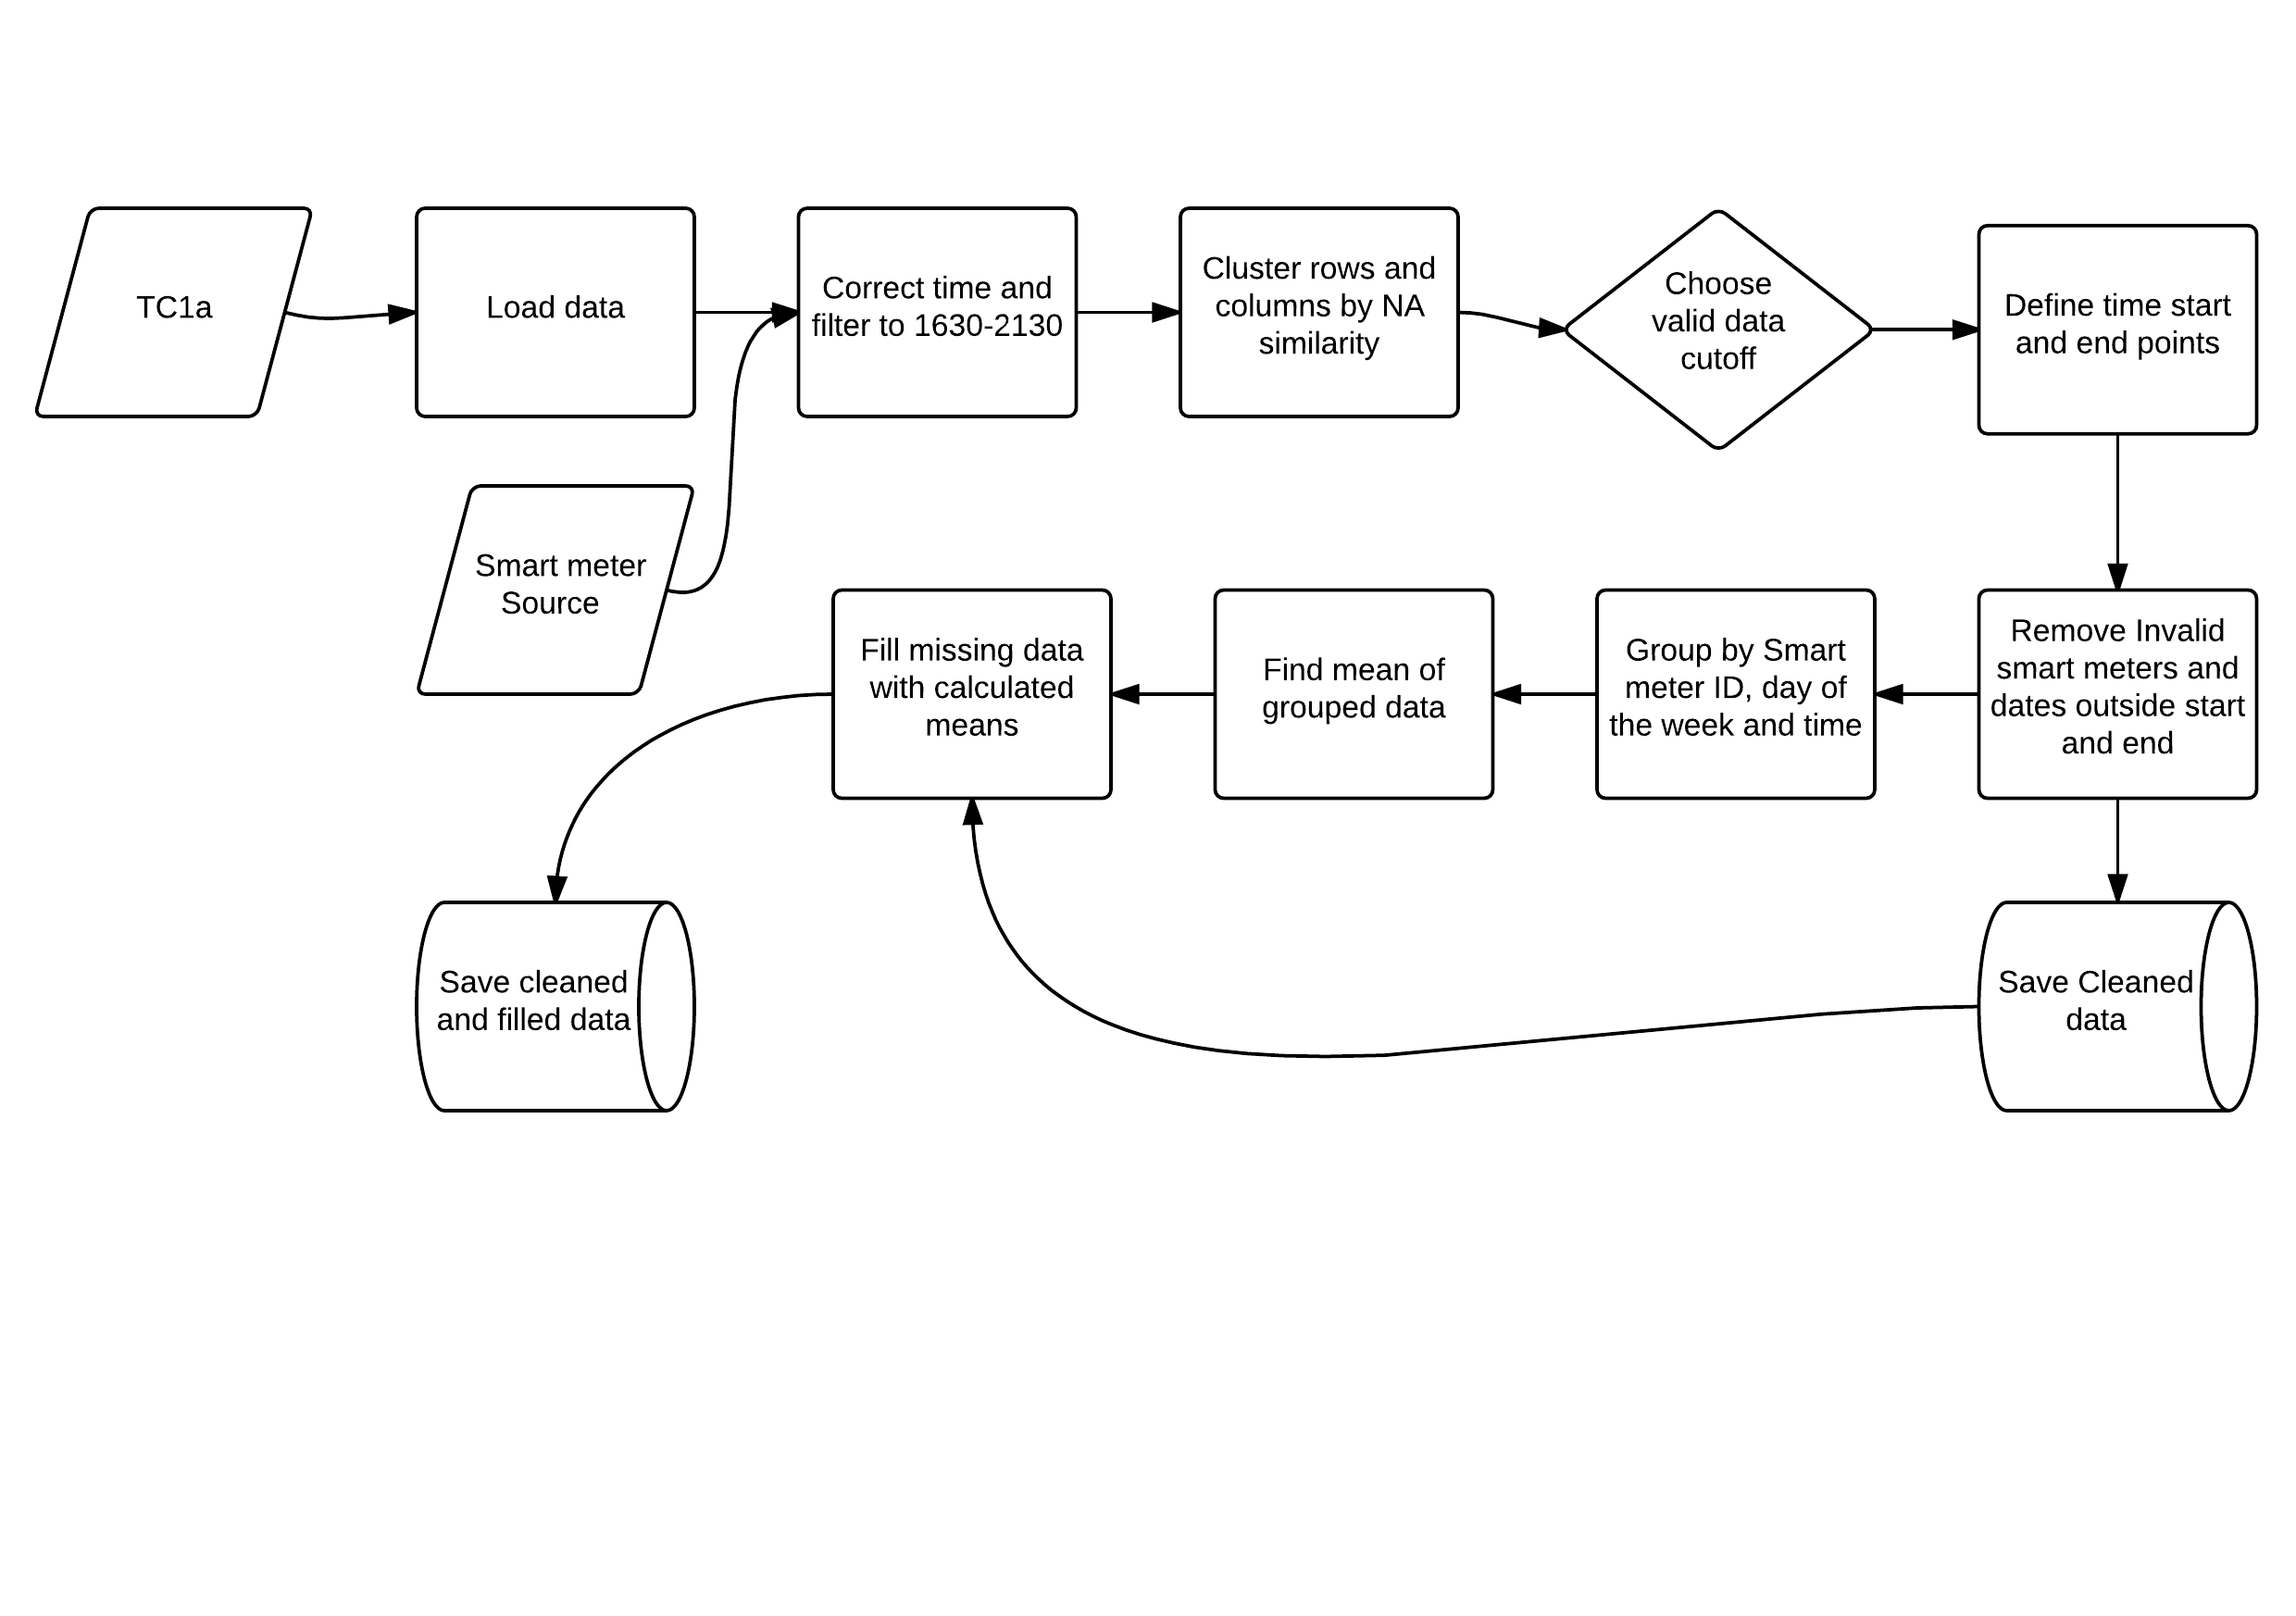
\includegraphics[width =\textwidth]{Figures/Appendix/DataCleaning.png}
    \caption[Data cleaning process]{Flow chart of the Data Cleaning Process}
    \label{fig:CleanFlow}
\end{figure}


\section{Method}

After loading the dataset, the timestamps need to be adjusted in order to take account of the different timezones used by the smart meters as mentioned in Chapter \ref{DataDesc}, so that when time filtering occurs, the correct time periods are taken for all smart meters and that usage is consistent across both smart meter brands. The time zone used will be local time, which is "Europe/London" from the the IANA timezone database \cite{iananumberresources1918}.

Once the timestamps have been adjusted the time periods will be filtered to the hours under investigation i.e 1600-2130. These hours have been chosen as this time period is of key interest to suppliers as consumption peaks when consumers return home in the evening, as a result the absolute value and variability is higher than other times during the day. This will reduce the amount of cleaning required to only that which will eventually be used and prevent confusing the cleaning process with irrelevant information. 

Once filtered the data is changed from long format to wide format in accordance with tidy data principles \cite{wickham2014}. This results in a data frame or matrix that is 8799 columns wide, with each column representing a smart meter plus the datetime column, and 1065 rows, where each row represents a half hour time period. The spreading process makes all smart meters present across all periods. Where smart meters did not send a time stamped data point either because they weren't installed or there was a transmission error, the data is classed as missing and filled with NA values.

In order to make sure the data is clean enough to be used, the data will be checked for missingness. Depending on the nature of the missingness different actions will be taken, low levels of missingness can either be removed, filled using an average, or filled using multiple imputation \cite{lee2013}. Due to the size of the dataset multiple imputation will not be considered as the resulting dataset will require a large amount of computation without having a clear payoff, however this approach can change once more information about the dataset is known. 

If the data is MNAR (Missing Not At Random) then the structure of the missingness will need to be analysed in order to find meter/day combinations that provide high levels of non-missingness, the remaining data will then be excluded from the rest of the process. The structure of the missingness will be visualised using an aggregated heatmap with both the time and smart meter axis ordered by hierarchical similarity. This method which was developed for this project takes a logical matrix where 1 represents valid data and 0 represents NA. The rows and columns of the matrix then make up individual vectors. The vectors of each row can be compared to each other using hierarchical clustering specifically the agglomerative Lance-Williams recursive clustering algorithm \cite{lance1967}. This clustering repeatedly groups the vectors by similarity, using the correlation matrix of the vectors, until all vectors have been grouped into a single cluster that represents the entire dataset. The order that the vectors were merged in created a new vector which is can be used to rearrange the vectors by hierarchical similarity, if both the time and smart meter dimensions of the data are rearranged the structural missingness of the data will be revealed see Figure \ref{fig:unordered} compared to Figure \ref{fig:ordered}. However with large datasets there can be so many vectors that the resulting organised matrix when visualised is difficult to interpret or computationally challenging to visualise. In order to resolve this, the orderd matrix is aggregated along the x and y axis by an appropriate amount, in the case of this data set the smart meters and time periods were aggregated by 5 each reducing the matrix by 25. This aggregation technique produces a value between 0 and 1 for an NA logical matrix. This technique is only appropriate after ordering by hierarchical similarity as it minimises the information loss caused by the aggregation process. The heatmap visualisation process will be used throughout the project in order to visualise similarity.

Using the heatmap the most valuable smart meters will be identified and isolated using a balance of least NA's and part of a large block of smart meters with a similar NA pattern. the next step will plot the minimum percentage of valid (non-missing) data required for each half-hour time period to be included in the dataset. After considering the volume/quality trade off on time periods, a cut off point will be chosen and all time periods which do not meet the minimum cut off criteria will be removed, and the same process repeated using smart meters. the resulting dataset will be a high quality subset of the original dataset, with relatively few missing values.

\subsection{Imputing missing values}
\label{sec:imputation}
As a large amount of the project involves the creation of similarity matrices, any NA values have the potential to invalidate the similarity score between any given smart meter pair. To prevent this the remaining NA's will be filled using the the half hour mean for that weekday for that smart meter for all values that are not NA. This runs the risk of some NA's being filled with unrealistic data, however the total number of NA's is likely to be so low that it doesn't have a significant effect on the overall result. In order to ensure that the data was as full as possible individual days that did not make the cut of minimum number of valid cells are re-included and the missing values included in the imputation process.

\section{Results}

Initial visual analysis of missingness was not very revealing as shown in figure \ref{fig:unordered}. In order to uncover any structure in the missingness, the rows and columns were ordered by the hierarchical similarity of the respective axis, this means that time periods that are most similar in their missingness are arranged together and smart meters that are most similar in their missingness are also arranged together. The resulting ordered missingness map is shown in figure \ref{fig:ordered}. It revealed that there was a high amount of missing data and that the data was Missing Not At Random (MNAR). In total 48\% of the dataset was missing values, according to the CLNR the majority of these losses were due to customer action \cite{howard2015}. To find which smart meters to extract, the amount of non missing data was plotted in the same order as the clustered smart meters, the results are shown in figure \ref{fig:breakpoints}. The results of this inspection showed that smart meters indexed between 2500 and 8100 had the most high quality data (a list of the actual smart meter ID's can be found in appendix \ref{app:smartmeters}). Extracting the smart meters using a high quality signal and plotting gives the image shown in figure \ref{fig:targetordered}. 

After selecting the initial block of smart meters for the experiment, the actual time periods needed to be selected in order give maximum amount of high quality data. A cut off of minimum number of valid data points in each time period was plotted, see figure \ref{fig:timecutoff}. A cut off was set at 90\% valid data. The process was then repeated with the smart meters as shown in figure \ref{fig:metercutoff}. The cut off for smart meter completion was 99\%. The final dataset was over 99\% valid data but covered only 25\% of the total dataset, a summary of the changes can be seen in table \ref{tab:nas}.


\begin{figure*}[ht]
\centering
\textbf{Cleaning the data}\par\medskip
\subfloat[Unordered missing data]{
  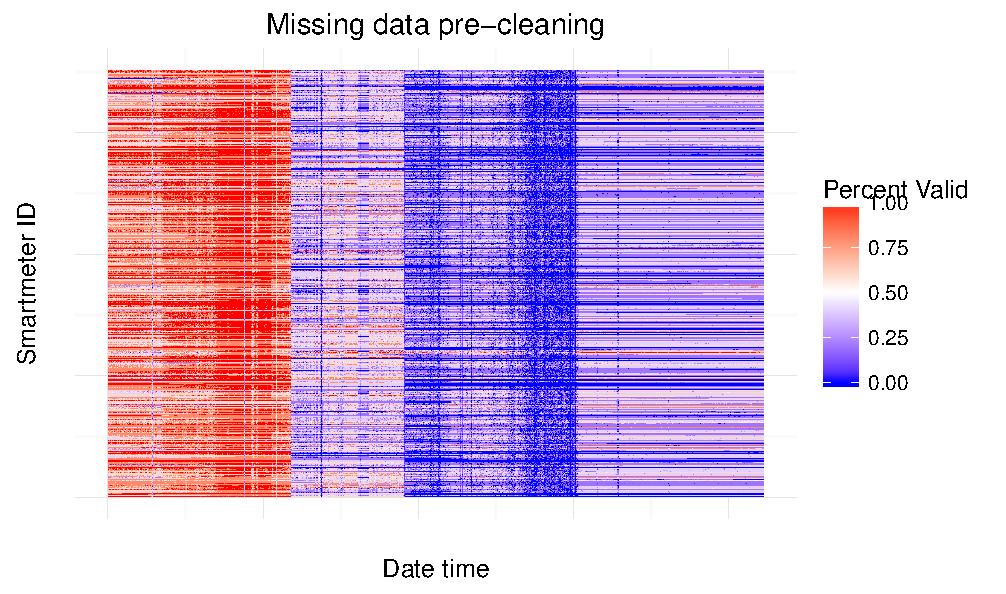
\includegraphics[width=0.49\textwidth]{Figures/unorderedPrecleaningmissing}\label{fig:unordered}
}
\subfloat[missing data with rows and columns ordered by similarity]{
  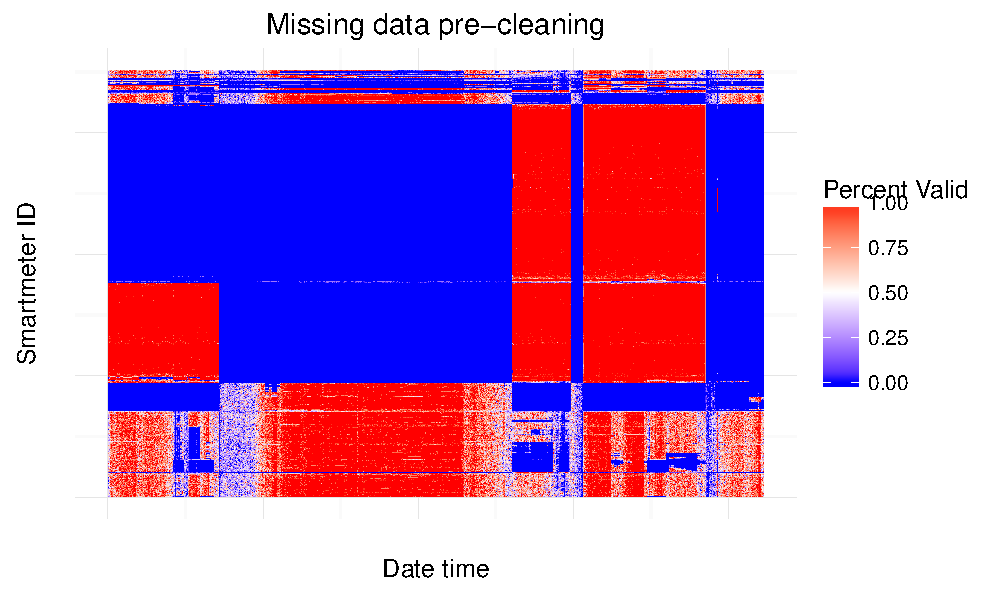
\includegraphics[width=0.49\textwidth]{Figures/Precleaningmissing}\label{fig:ordered}
}

\subfloat[Identifying smart meters that have similar high quality data]{
  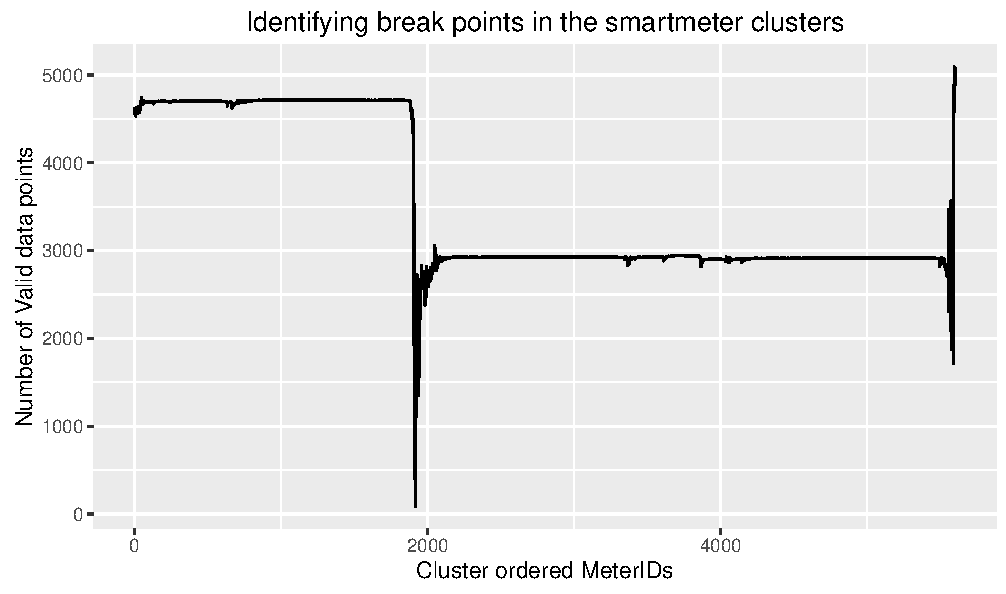
\includegraphics[width=0.49\textwidth]{Figures/breakpoints}\label{fig:breakpoints}
}
\subfloat[Missing data of the selected smart meters in chronological order]{
  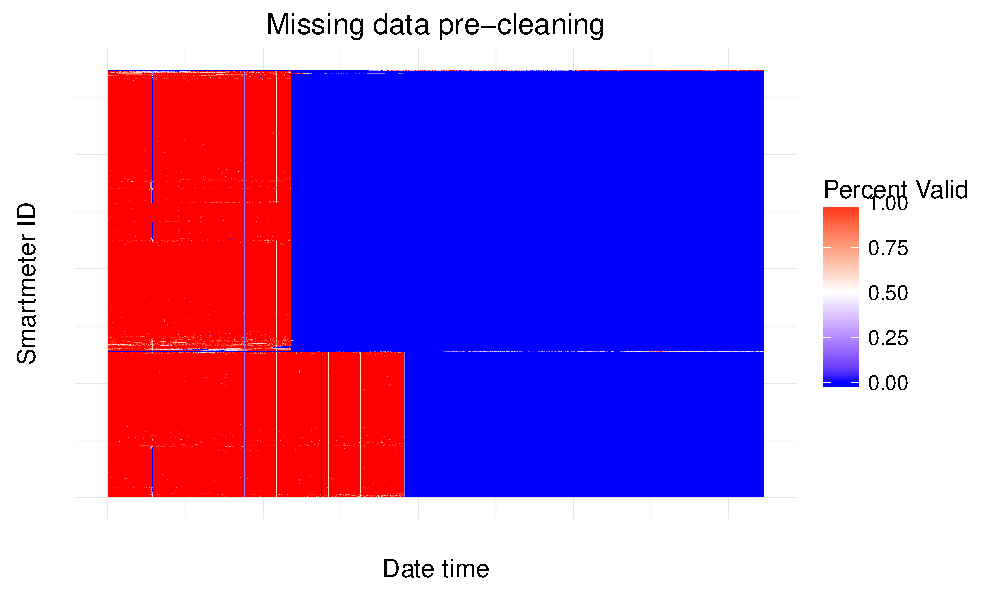
\includegraphics[width=0.49\textwidth]{Figures/LowerPrecleaningmissing}\label{fig:targetordered}
}
\caption[Cleaning the data]{This series of figures shows how the Sub-set of smart meters and time periods were chosen from the raw data.}
\label{fig:dataclean}
\end{figure*}

\begin{figure*}[ht]
\centering
\subfloat[The number of time periods remaining if there is a minimum cut off for valid data]{
  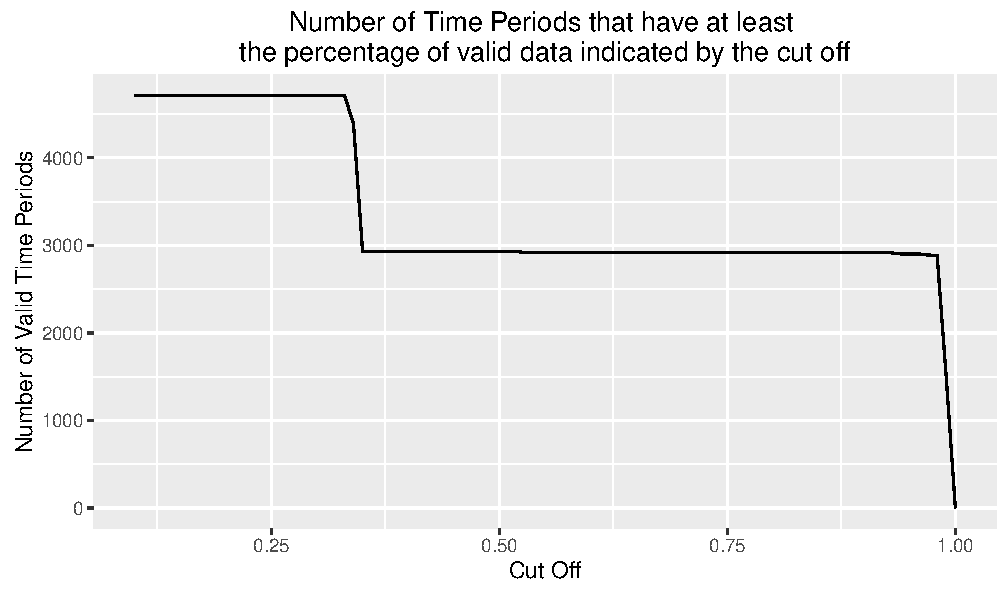
\includegraphics[width=0.49\textwidth]{Figures/NAtimeperiodslowerclust}\label{fig:timecutoff}
}
\subfloat[The figure shows how many smart meters remain if requirements are put on the percentage of time periods that must be valid for the smart meter to be included. As can be seen, the number is much more stable than for the time period figure, however this is mostly due to the time periods have been cleaned first.]{
  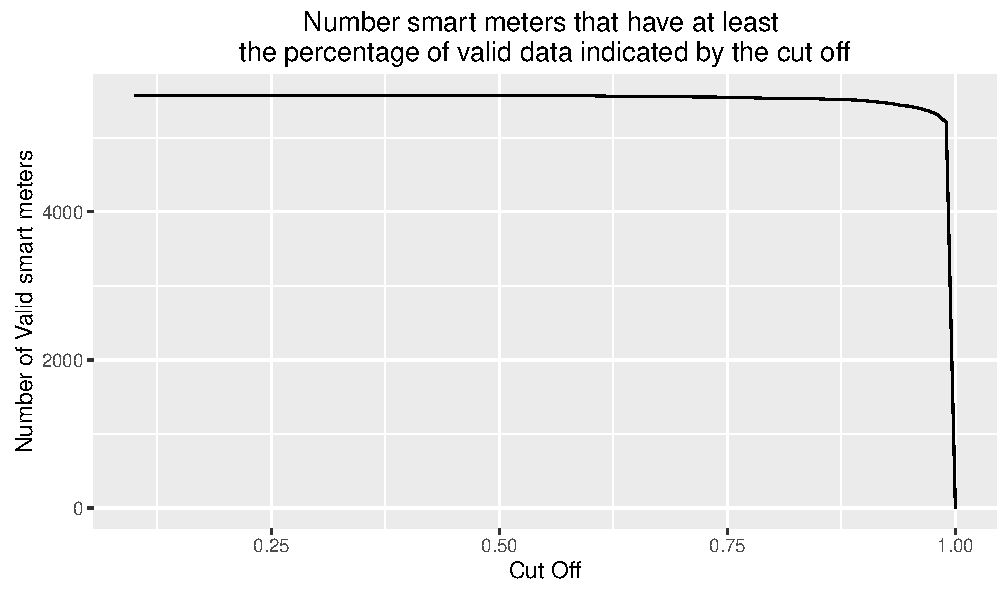
\includegraphics[width=0.49\textwidth]{Figures/NAsmartmeters}\label{fig:metercutoff}
}
%\caption{This series of figures shows how the Sub-set of smart meters and time periods were chosen from the raw data.}
\label{fig:dataclean2}
\end{figure*}


After cleaning there are 242 complete days of 12 half hour periods from 1600 to 2130, there are 239 days that have a comparison day 1 day earlier and 233 days that have a comparison day 1 week earlier and . The total dataset has 14386 NA values.
the dates "2011-06-29", "2011-10-31", "2011-12-12" are missing from the data set due to low valid values further details can be seen in table \ref{tab:nas}. After the  imputation of data described in \ref{sec:imputation}, the 3 missing days were admitted to the data set and  all NA values were filled in.

\begin{table}[ht]
\centering
\begin{tabular}{|l|l|l|l|} \hline
             & Pre Cleaning & Post Cleaning & \% Reduction \\ \hline
Time periods & 10565        & 2915           & 72\%      \\ \hline
Smart Meters & 8790         & 5209          & 41\%      \\ \hline
NA's         & 48\%         & 0\%           & 100\%     \\ \hline
Nodes        & 8798         & 5260          & 40\%      \\ \hline
\end{tabular}
\caption{Summary of the data removal that took place in the cleaning process to reduce the amount of NA's in the dataset.}
\label{tab:nas}
\end{table}

\FloatBarrier

\section{Basic consumption patterns}
\label{sec:basicconsum}
A brief visual analysis of the data shows a few key insights. Figure \ref{fig:PortfolioLoad} breaks out the the load profile per week day, it shows that independent of day of the week all evening peaks look roughly the same. However the weekend peak is slightly before the week days, peaking about an hour earlier, in addition Saturday has the lowest average consumption. Aggregating the consumption to total kWh per day and comparing daily consumption across months, a clear pattern emerges as shown in figure \ref{fig:DailyConsumption}. As the days get darker and colder energy consumption increases, this is intuitive as people are more likely to spend time indoors, have the lights on, and use heating. 

As this project relies on finding correlations between smart meters, it is interesting to look at how much correlation there is within smart meters. This means looking at a single smart meter's correlation with itself across multiple days. Figure \ref{fig:MeanAbsCorr} shows a density distribution of the absolute correlation across 50 randomly sampled smart meters. If people led very regimented lives and did exactly the same thing every day then the average score would be 1, conversely no pattern would get a score of 0. The distribution shows a mean score of 0.3 which is quite low, suggesting that there is not strong structure among individual energy consumption. The unexpectedly low levels of correlation may be due to the low absolute levels of electricity consumption relative to the total energy consumption for the household, see Appendix \ref{sec:Energybreakdown} for more details and discussion. 


\begin{figure}
    \centering
    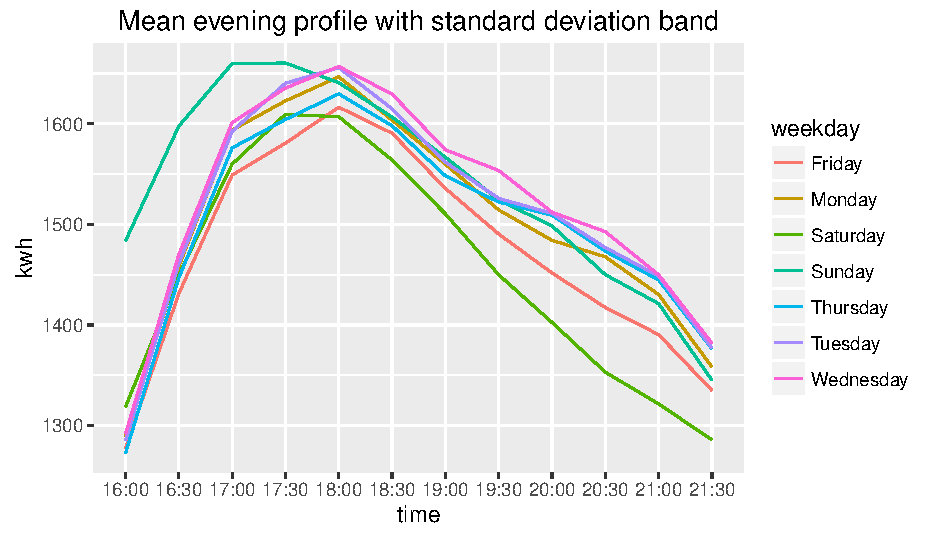
\includegraphics[width = \textwidth]{Figures/Results/PortfolioLoad}
    \caption[Portfolio load by day]{The figure shows the portfolio load across all weekdays, as can be seen the load on the system peaks at about 1800 across all weekdays. The weekend peak is slightly earlier, peaking about an hour earlier, in addition Saturday has the lowest average consumption.}
    \label{fig:PortfolioLoad}
\end{figure}

\begin{figure}
    \centering
    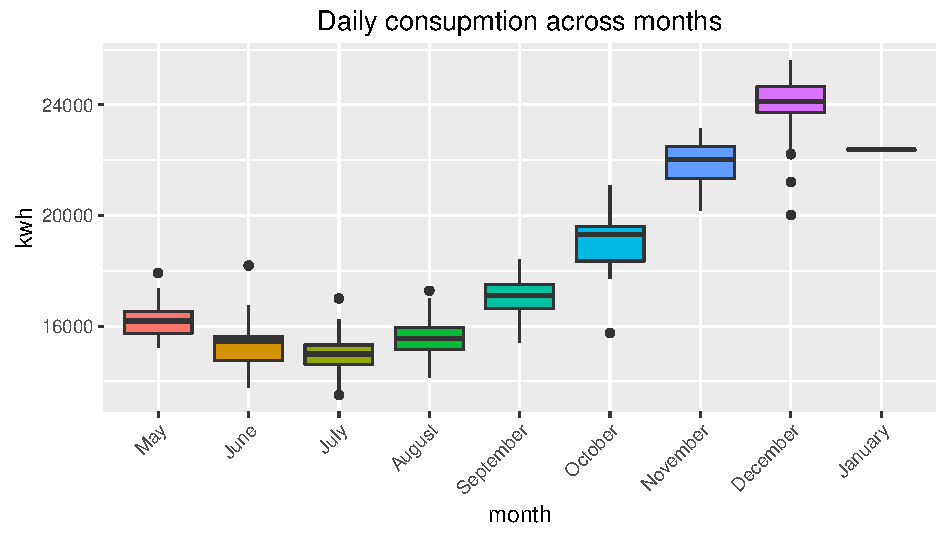
\includegraphics[width = \textwidth]{Figures/Results/DailyConsumptionMonths}
    \caption[Daily consumption across months]{As can be seen the consumption of electricity increases as the days get darker and colder, requiring more energy in the form of heat an light.}
    \label{fig:DailyConsumption}
\end{figure}

\begin{figure}
    \centering
    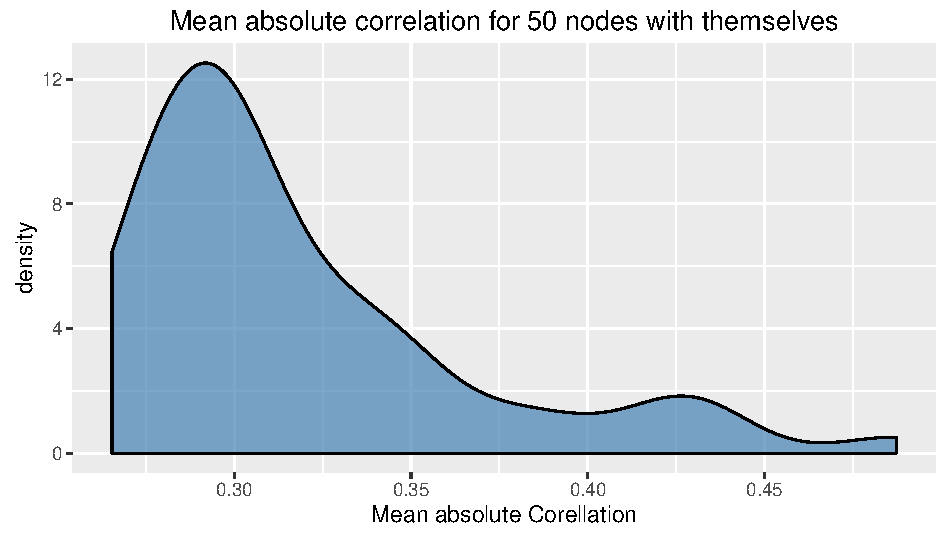
\includegraphics[width = \textwidth]{Figures/Results/MeanAbsCorr}
    \caption[Node Mean absolute correlation]{This figure was made by Taking a node and find it's mean absolute correlation with itself across all days, and repeating with 50 randomly selected nodes. The resulting vector of scores are then made into a density plot. the right skew shows that the majority of nodes have very low self-correlation suggesting that there is little fixed pattern to behaviour.}
    \label{fig:MeanAbsCorr}
\end{figure}

\section{Summary}

This chapter explains the method and results of the cleaning process for the TC1a dataset. The dataset had 48\% missing values during the evening peak period this was reduced to slightly over 0\% and the remaining missing values were imputed using node/day/time mean. Cleaning used a combination of hierarchical clustering,visualisation and minimum data quality decisions in order to produce the final dataset.



\chapter{Methodology}
\label{Method}

The process for predicting the portfolio load using graph classification is performed in several stages, an overview of which can be seen in Figure \ref{fig:ProcessFlow}. The following method is written in order to increase understanding of the project and aid reproducibility. The methodology developed in this chapter ensures that the resulting graphs are made in efficiently and that clustering maximises the modularity of each graph. Checks for the probability distributions are discussed to ensure that the findings are not due to spurious relationships in the data. Finally the models developed are discussed, and where appropriate, defined mathematically and the evaluation metrics discussed.

\begin{figure}[ht]
    \centering
    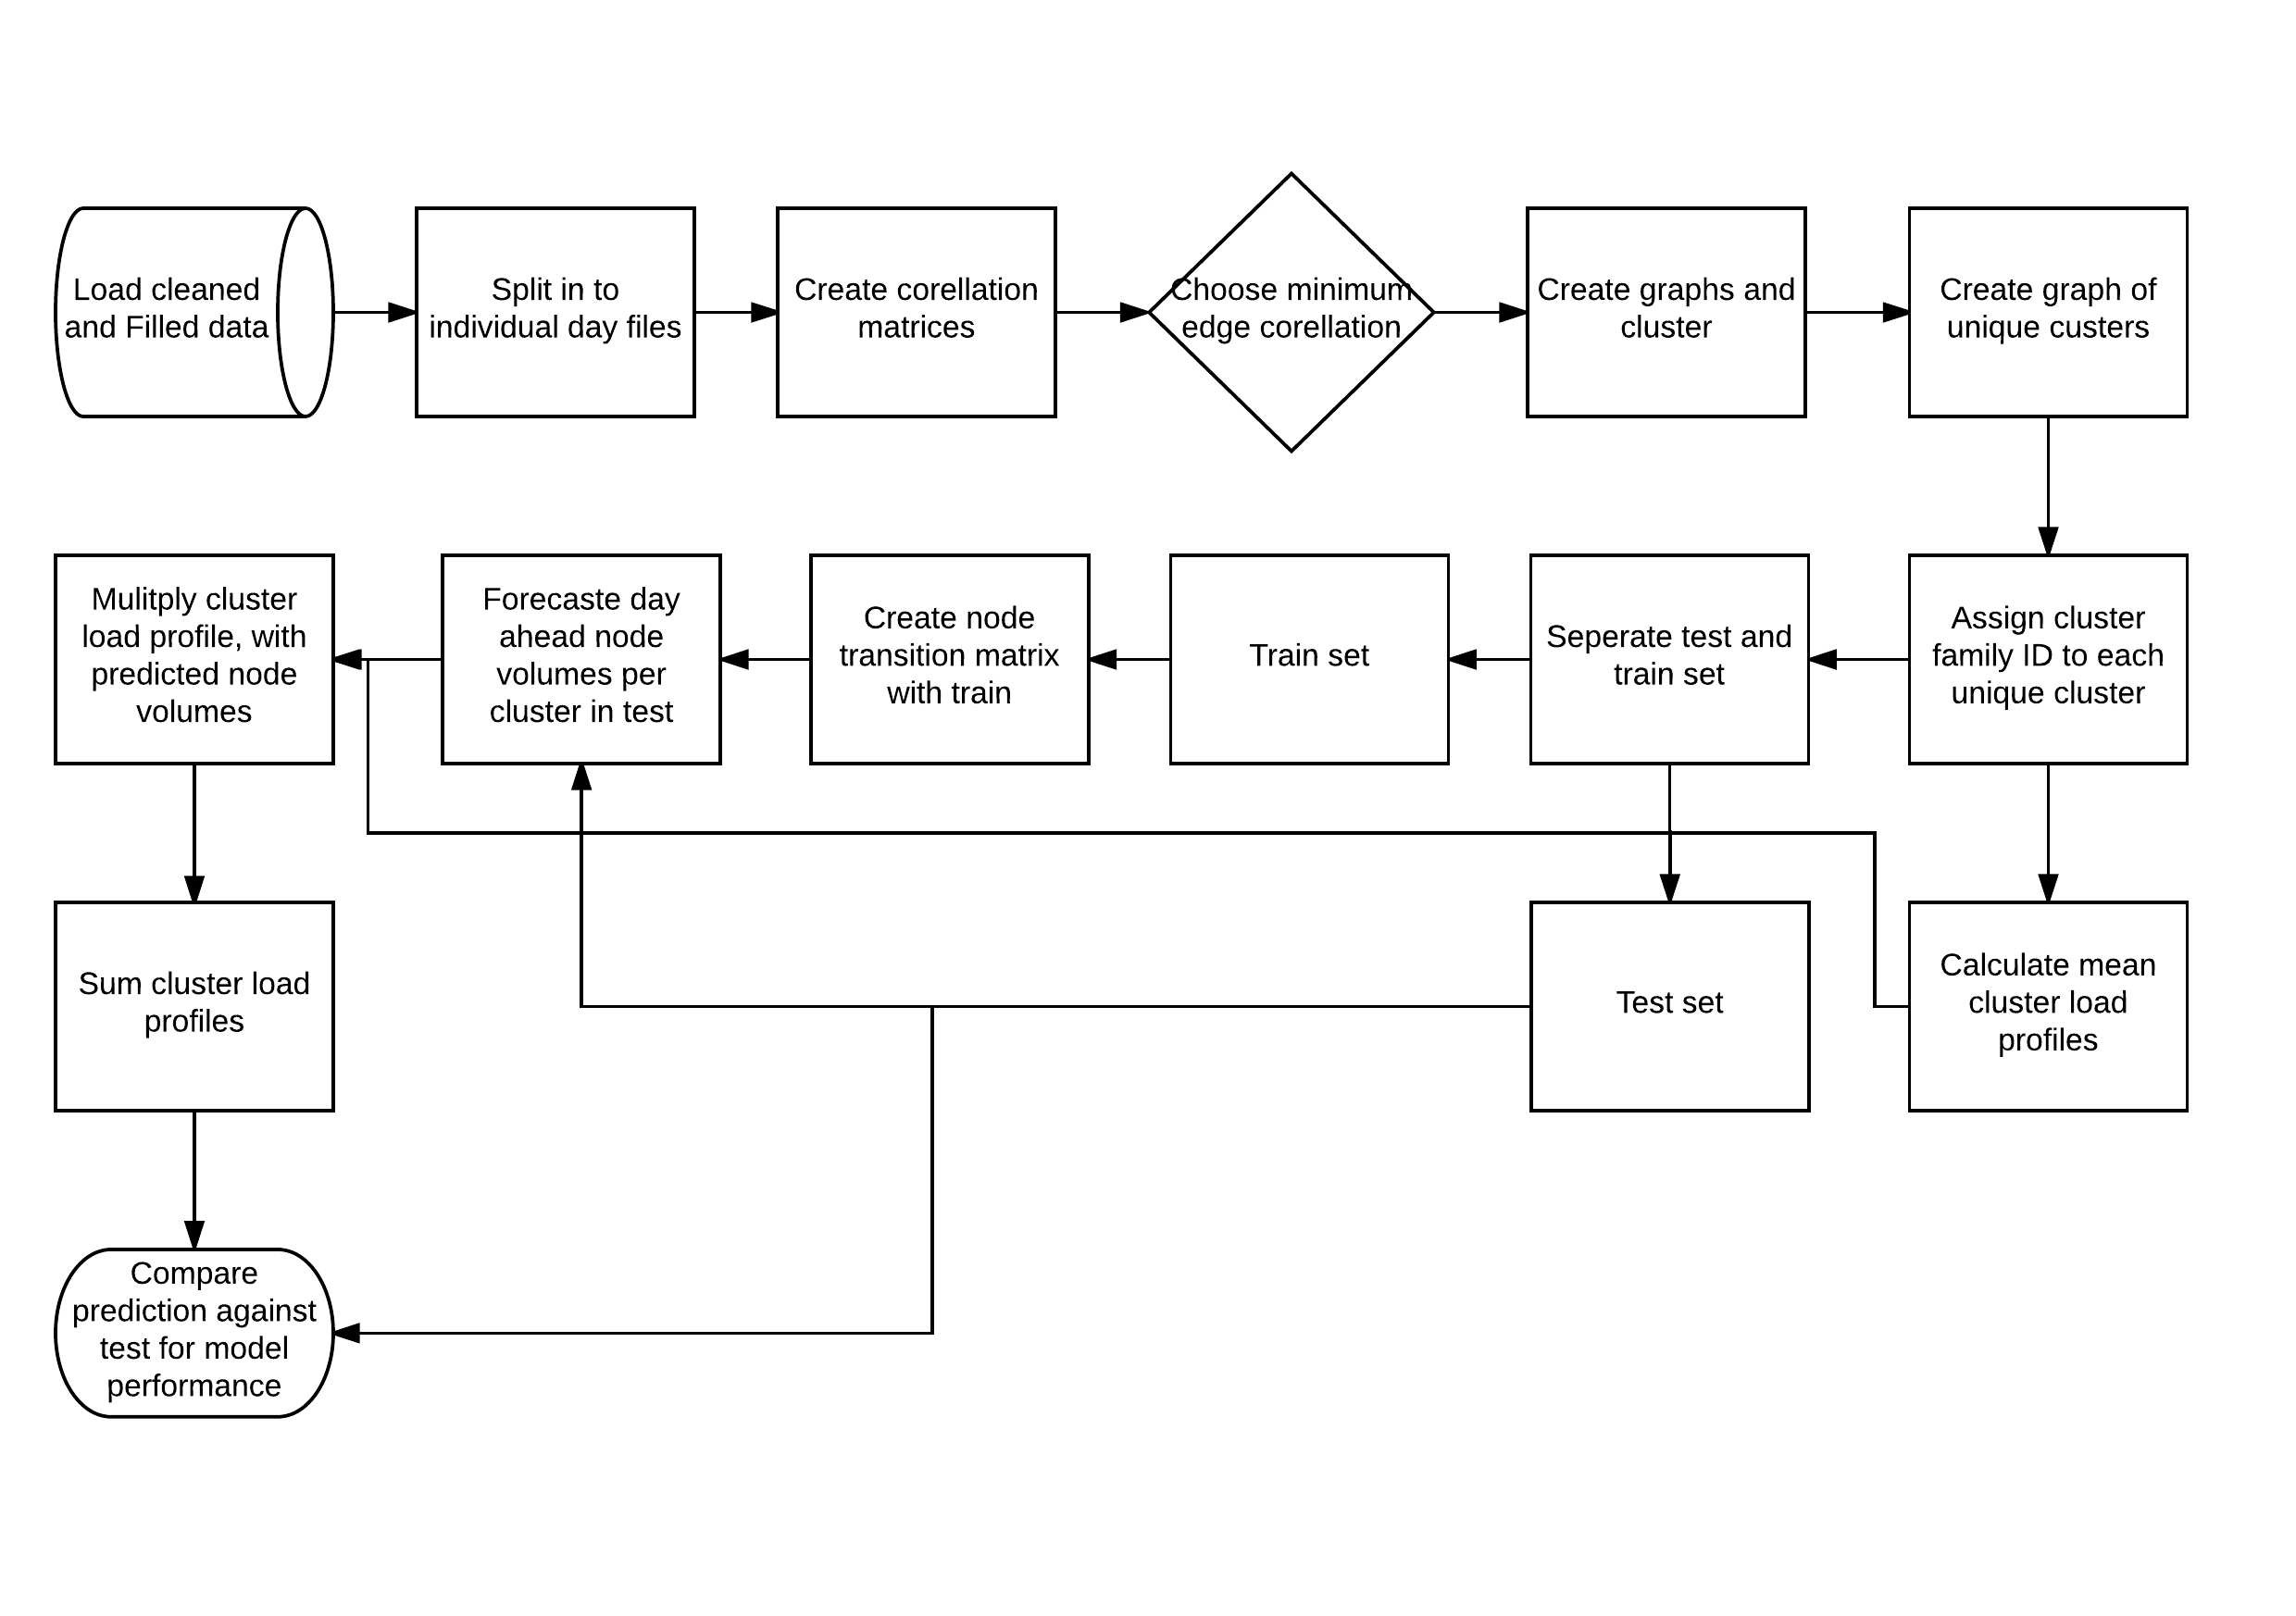
\includegraphics[width =\textwidth]{Figures/Appendix/Thesisprocess.png}
    \caption[Project process]{Flow chart showing the process of generating and testing the predictive model once the data has been cleaned}
    \label{fig:ProcessFlow}
\end{figure}


\section{Creating correlation matrices}
\label{sec:cormat} \label{sec:CormatEdge}
The graph building block is the similarity metric that forms the link between smart meters. As was shown in Section \ref{sec:basicconsum}, the distribution of power is not normal, meaning that Spearman's correlation \cite{spearmansrankcorrelationcoefficient2016} was preferred instead of Pearson's. Spearman's rho is a non-parametric test allowing for non-normal distributions, it uses ranks instead of raw scores. Two formulas for Spearman's correlation are shown in equations \ref{eq:spearmans1} to \ref{eq:spearmans3}, rank is shown by $rg_x$ and $rg_y$. Equation \ref{eq:spearmans1} is the base version of Spearman's rho whilst \ref{eq:spearmans2} is a version which can be used if the ranks are all distinct integers, in this project equation \ref{eq:spearmans1} is used.

As there are 5260 nodes in the dataset the resulting matrix contained 2.7 million elements, of varying degree's of correlation, the ordered correlation matrix for 09-08-2011 is shown in Figure \ref{fig:day100corplot}. By creating the correlation matrices for all days, it reduces the computational load for making changes later on in the processing pipeline, such as changing the minimum correlation requirements for link and rebuilding the graphs. Each correlation matrix was over 200mb, together the total size of all the correlation matrices was over 40Gb.

\begin{equation}
\label{eq:spearmans1}
    \rho = \frac{cov(rg_x,rg_y)}{\sigma_{rg_x}\sigma_{rg_y}}
\end{equation}

\begin{equation}
\label{eq:spearmans2}
    \rho = 1- \frac{6 \sum d_i^2}{n(n-1))}
\end{equation}

\begin{equation}
\label{eq:spearmans3}
    d_i = rg(X_i)-rg(Y_i)
\end{equation}

\begin{figure}
    \centering
    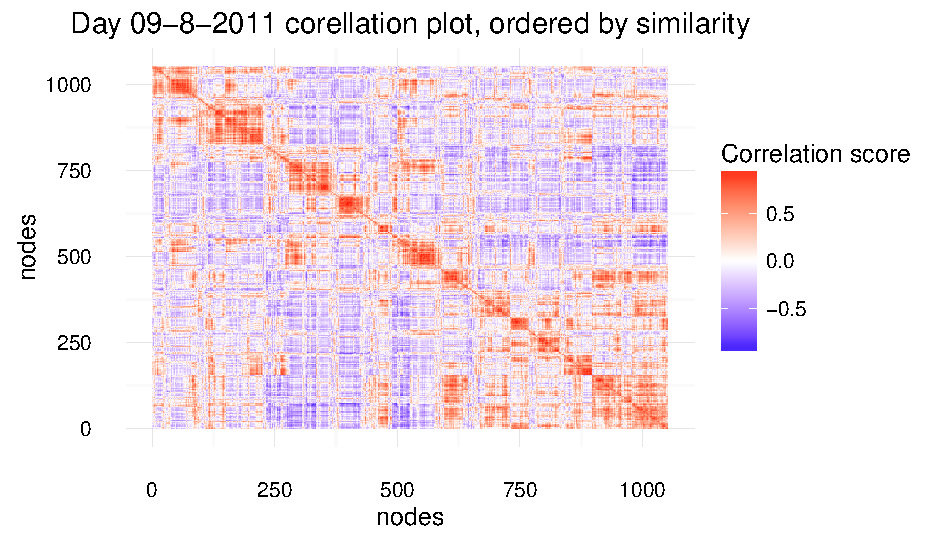
\includegraphics[width=\textwidth]{Figures/Results/day100Corplot}
    \caption[Example corellation matrix]{The correlation matrix of 09-08-2011 with the nodes organised by hierarchical similarity.}
    \label{fig:day100corplot}
\end{figure}


\section{Finding an appropriate  edge correlation cut off point}
As the dataset has 5260 nodes the the number of edges in a fully connected graph is almost 14 million which is intractable on a normal machine especially as the edges are weighted. It is also doubtful how much extra information will be gained using a fully connected graph instead of using a graph where the edges of the adjacency matrix is determined by a cut off distance. In order to measure the effect of a cut off value the number of edges and non isolated nodes were counted in each graph for a given correlation cut off, starting at 0.1 and increasing by 0.05 up to 1. In order to avoid constructing a large number of highly complex graphs the correlation matrices of each day were turned into logical matrices using the form $A>x$ where $A$ is the correlation matrix and $x$ is the cut off point, the number of isolated nodes is then equal to the number of rows/columns with a sum of 0 (the diagonal of the correlation matrix has already been set to zero).

The results of edge analysis are shown in Figure \ref{fig:EdgeNodeAnalysis}. They reveal that that the number of edges and non-isolated nodes are relatively consistent across the graphs. Sub Figure \ref{fig:Meanedges} shows that the number of edges decreases approximately quadratically with increasing minimum correlation. It can be seen that there is a small right skew in the data as there is a visible difference between the mean and the median, the standard deviation of the edge number is approximately 10\% of the mean. 

Sub Figure \ref{fig:Meannodes} shows the mean number of nodes for each cut off point. Node number analysis showed very little variation with a negligible standard deviation and a median that is the same as the mean. It is clear that the total number of non-isolated nodes stays almost constant up to quite high levels of correlation before dropping off steeply to zero. Comparing the percentage of non-isolated nodes against the percentage of total edges as in Figure \ref{fig:Edgenodeperc} shows that the percentage difference between the two grows quite large, Figure \ref{fig:EdgeNodeDiff} shows the difference is maximised at a cut off of 0.8. 

The results of this analysis suggests that using 0.8 as a cut off will provide the highest number of non-isolated nodes for the lowest number of edges. However it should be noted that although the number of non-isolated nodes is low, experimenting with various graphs reveals that there are many nodes in small unconnected sub graphs of two or three, therefore the cut off point will be set at a more conservative 0.7. This makes a much more highly connected graph but is still tractable. 

With the cut off point chosen at 0.7 all graphs can be generated and community detection performed.

\begin{figure*}[ht]
\centering
\textbf{Number of edges analysis}\par\medskip
\subfloat[]{
  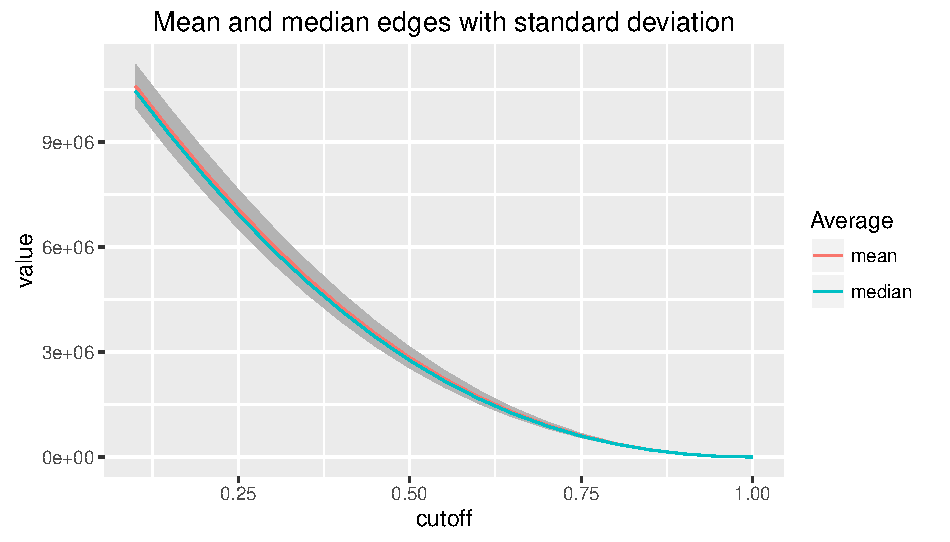
\includegraphics[width=0.49\textwidth]{Figures/Results/Meanedges}\label{fig:Meanedges}
}
\subfloat[]{
  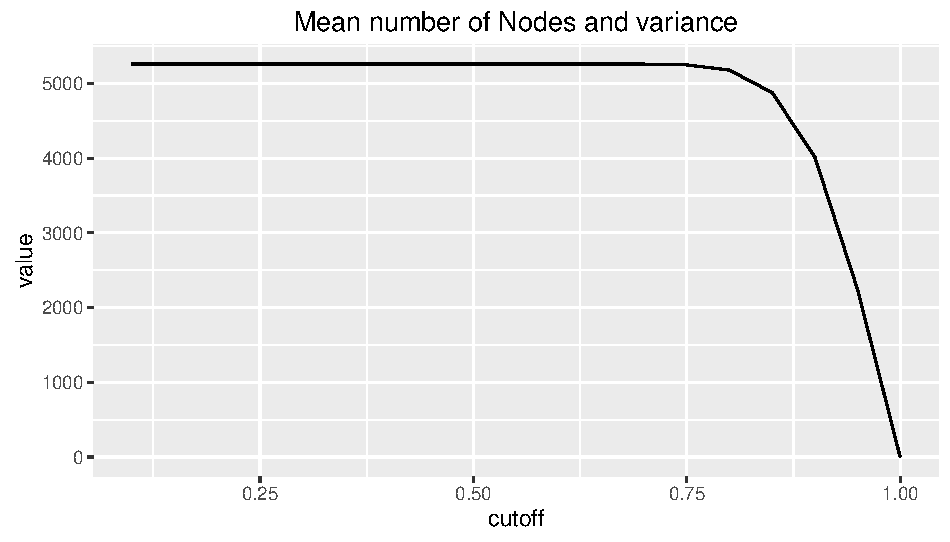
\includegraphics[width=0.49\textwidth]{Figures/Results/Meannodes}\label{fig:Meannodes}
}

\subfloat[]{
  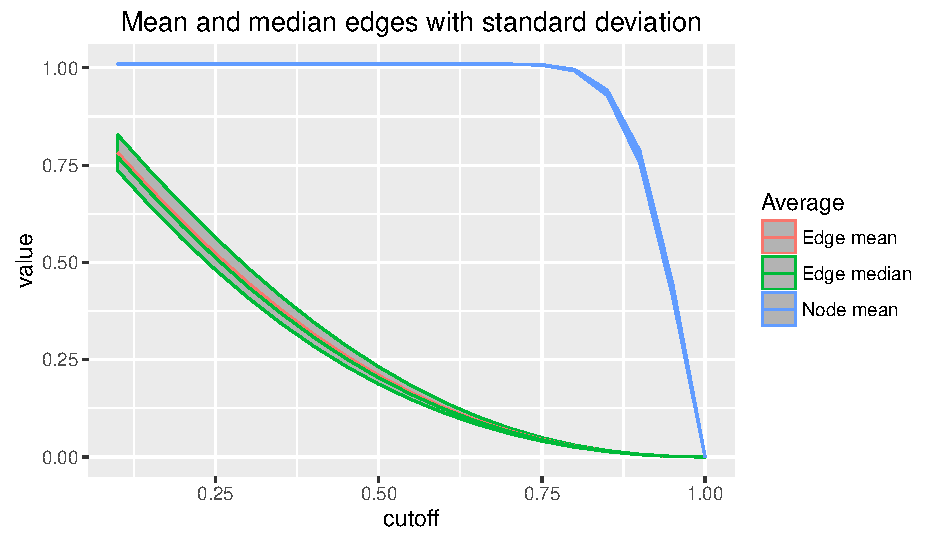
\includegraphics[width=0.49\textwidth]{Figures/Results/Edgenodeperc}\label{fig:Edgenodeperc}
}
\subfloat[]{
  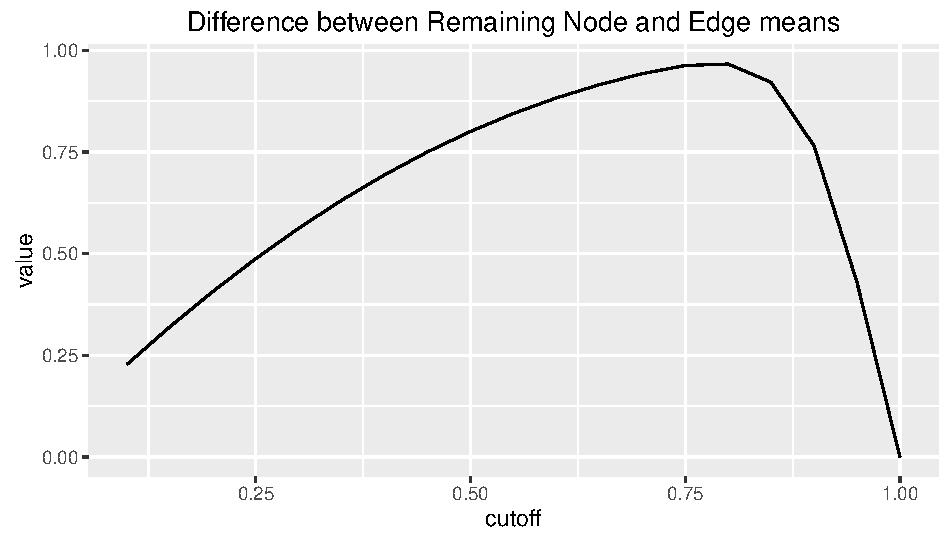
\includegraphics[width=0.49\textwidth]{Figures/Results/EdgeNodeDiff}\label{fig:EdgeNodeDiff}
}
\caption[Number of edges analysis]{Analysis of the number of edges and nodes for given correlation cut offs, across all 233 days, shows a relatively low standard deviation and slight skew with the number of edges. The number of nodes has an extremely low standard deviation, comparing the difference between the percentage remaining nodes and edges sees that the value is maximised at a correlation cut off of about 0.8. }
\label{fig:EdgeNodeAnalysis}
\end{figure*}



\subsection{Comparison with an Erdos-Renyi graph}
The Erdos-Renyi (ER) graph, developed by P Erdos and A Renyi in 1959 \cite{erdos1959}, showed that for any graph $\mathcal{G}$ had an equally likely probability of appearing when the number of vertices $v$ and edges $m$ were fixed, this is the so called GnM model, which is a graph $G$ with $n$ nodes and $M$ edges. In this model each element in the adjacency matrix has an equal probability of being present, that is $\frac{2m}{v(v-1)}$. In 1960 Erdos and Renyi explored the properties of the GnP \cite{erds1960}, which is a graph $G$ with $n$ nodes and each edge has an equal probability $P$. They found that above a critical level there was a high probability of the graph being connected (no isolated nodes) see equation \ref{eq:connected}. 

\begin{equation}
\label{eq:connected}
    p>\frac{(1+\epsilon)ln \; n }{n}
\end{equation}

An ER graph represents random noise, we will test whether the smart meter data has a significantly different number of isolated nodes than an ER graph for the same number of edges. If there is a significant difference between the graphs then it can be inferred that there smart node graphs are not random. This test will be done by generating 20 different ER graphs with the same number of edges as the mean number of edges for each cut off point for the smart meter data. The mean number of non-isolated nodes will then be compared with the mean number from the smart meter data using a paired \textit{t}-test.

\begin{figure}
    \centering
    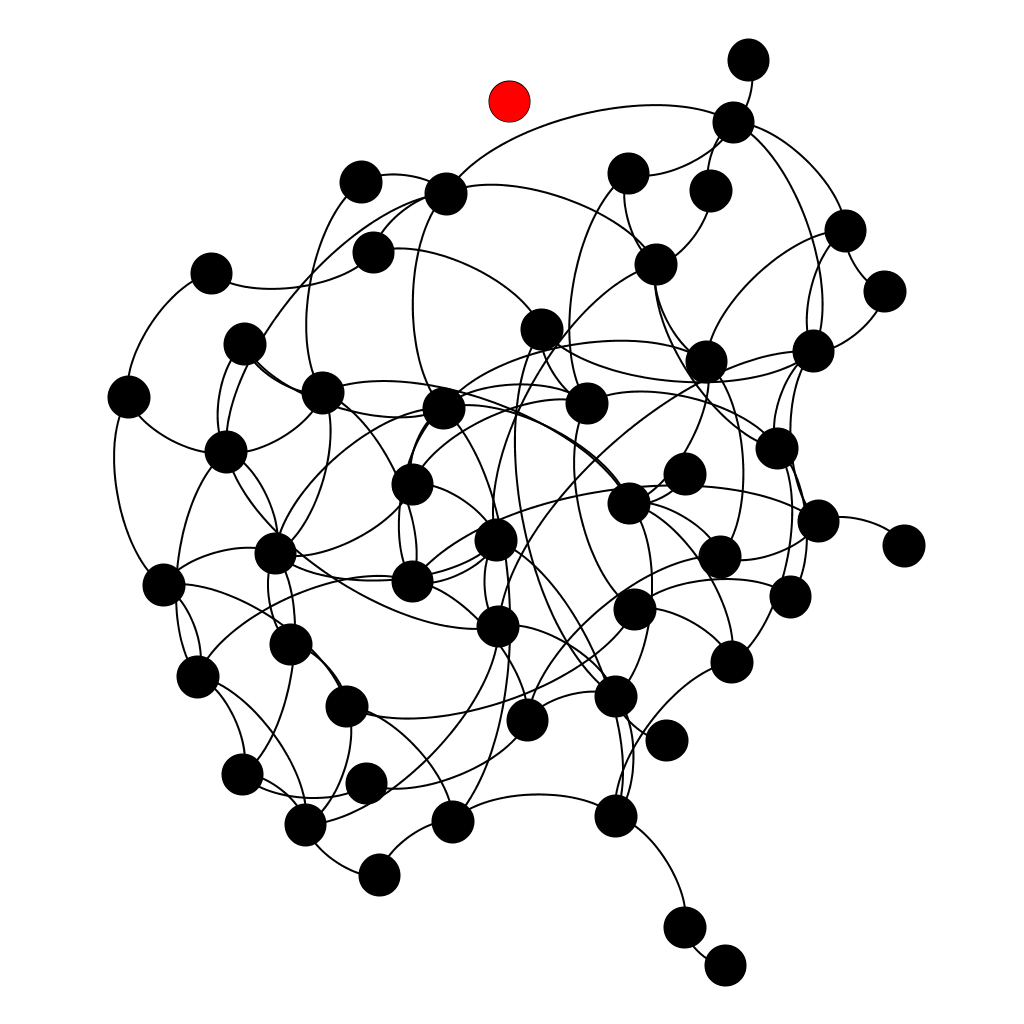
\includegraphics{Figures/Method/RandomGraph}
    \caption[Example Erdos-Renyi Graph]{An example of an Erdos-Renyi graph, generated with 50 nodes and 100 edges, note that the node highlighted in red has no edges and is separated from the the rest of the graph, despite the fact that the conditions in equation \ref{eq:connected} have been met. }
    \label{fig:RandomGraph}
\end{figure}

\section{Creating the graphs}
\label{chap:creategraph}

The correlation between the nodes will be converted in to a distance using $\sqrt(2(1-\rho))$ as popularised by Mantegna \cite{mantegna1999} and then into a weighted undirected graph. This distance metric is chosen over other metrics, such as euclidean distance, Manhattan or any other choice as it has been previously applied in a a similar time based setting, and that correlation is an a conceptually intuitive way to measure similarities over time as opposed to, for example, 12 dimensional euclidean space.  Once in graph form Community detection will be performed. The community detection algorithm used will be The Louvain algorithm, it was chosen from 4 different methods Fast Greedy, Walktrap, Louvain and Infomap mentioned in sections \ref{sec:commdetect}. The choice was made by selecting 50 random graphs and performing clustering on them using the different methods and then inspecting the resulting modularity scores and run time results. The results of the test shown in Figure \ref{fig:ChooseAlg} shows that although the results are similar for Walktrap, Infomap and Louvain, Louvain has a much lower average runtime than the other algorithms, therefore the Louvian algorithm was chosen.

\begin{figure*}[ht]
\centering
\subfloat[]{
  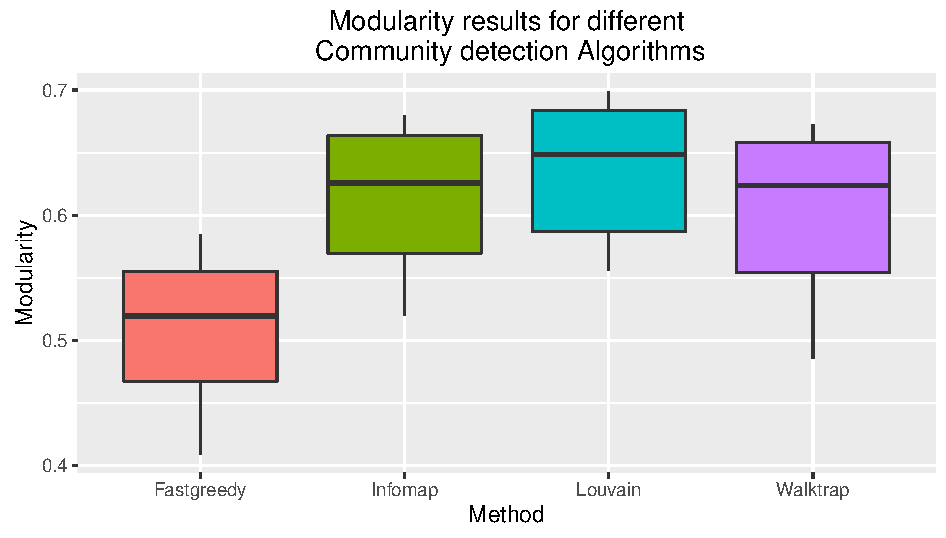
\includegraphics[width=0.80\textwidth]{Figures/Results/CommModComp}\label{fig:CommModComp}
}

\subfloat[]{
  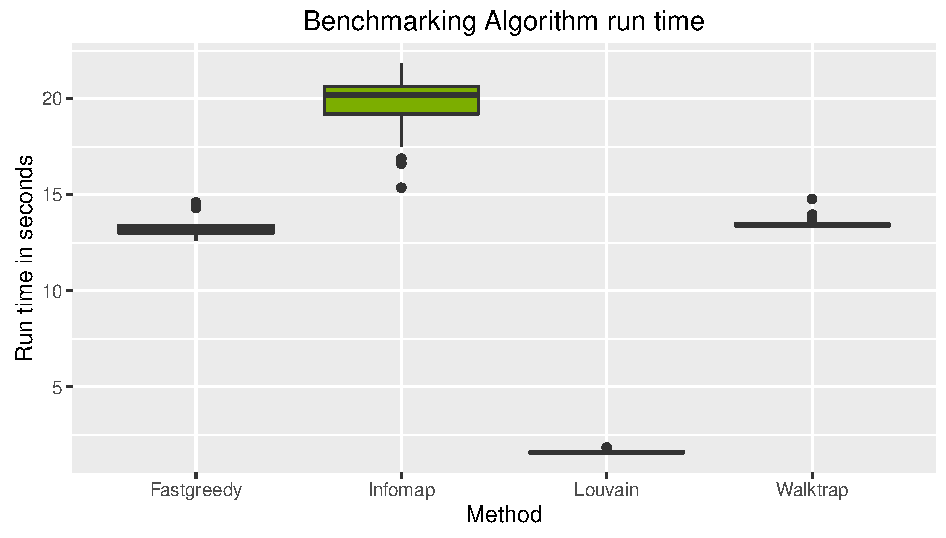
\includegraphics[width=0.80\textwidth]{Figures/Results/AlgorithmTimes}\label{fig:Algtime}
}

\caption[Cluster Family Load Profiles]{ Benchmarking the four target algorithms, shows that Walktrap, Infomap, and Louvain are all statistically similar in performance with Louvain getting slightly better results, however Louvain is considerably faster when it comes to detecting clusters}
\label{fig:ChooseAlg}
\end{figure*}

\section{Labelling clusters}
\label{sec:labelClust}

The result of the graph creation process will be 246 correlation matrices and corresponding graph structures, each graph will have a different number of clusters of different sizes and the clusters will all have slightly different profiles across days. This leads to the labelling problem of how to group various different but similar items into a set of finite groups when the group labels are unknown. In order to find our which clusters are similar to each other, and are part of the same cluster family the mean load profile of each cluster will be found and the same process used to discover the clusters discussed in Section \ref{sec:cormat} and \ref{chap:creategraph}, this will create clusters of clusters that will form the cluster families used to identify consistent behaviour types throughout the period.  The main difference will be that the cut off for the creation of a link will be set higher due to the inherently higher levels of correlation that will be present in the clusters, due to the averaging effect of clustering. This Process will create an $\mathbf{C_f}x\mathbf{C_f}$ correlation matrix where $\mathbf{C_u}$ is the total number of unique clusters across all days. 

In the creation of clusters not all nodes will behave similarly, certain clusters will appear only once, or contain a very small number of nodes, these clusters create noise which does not provide any value. To prevent a situation with a large number of clusters where only a small number are useful a "Node Soup" will be created. This soup will form a cluster of all clusters that contain either less than 50 nodes, or whose cluster family contains less than 1\% of the total node volume across the whole time frame.


\subsection{Load profiles}
\label{sec:LoadProfiles}
Once nodes have been assigned to clusters the load profile of each cluster can be calculated, four metrics will be used for visualisation of the cluster families and individual clusters and will define their characteristics and the common behaviour of the group as a whole. For the prediction part of the project the mean profile will be used as this has the advantage that the product of the mean load profile and the number of nodes in that cluster summed across all clusters is equal to the total load profile.

\begin{enumerate}
\itemsep0em 
\item Sum: The total kWh used by the cluster
\item Mean: The mean kWh of the nodes in the cluster
\item Median: The median kWh of the nodes in the cluster
\item Variance: The variance of the kWh of the nodes in the cluster
\end{enumerate}

\section{Probability distributions}

\subsection{Cluster transition}
\label{sec:Clusttrans}
An important stage of exploring how energy is consumed is by looking at the probability of nodes transitioning from one cluster to another across consecutive days. This analysis will create a transition matrix like that shown in Table \ref{tab:trans}, it can also be shown in graph form as in Figure \ref{fig:exampletrans}. 

\begin{table}[ht]
\centering
\begin{tabular}{|l|llll|} \hline
   & $c_1$  & $c_2$  & $c_3$  & $c_4$  \\ \hline
$c_1$ & 0.5 & 0   & 0   & 0.5 \\
$c_2$ & 0   & 0.8 & 0.2 & 0   \\
$c_3$ & 0   & 0.2 & 0.7 & 0.1   \\
$c_4$ & 0   & 0   & 0.1   & 0.9  \\ \hline
\end{tabular}
\caption[Example Cluster Transition matrix]{The transition matrix shows how a possible cluster transition could look. cluster $c_1$ will eventually be consumed by $c_4$. $c_2$ and $c_3$ have a constant low level exchange between each other. $c_4$ and $c_3$ also have a low level of exchange which means that $c_4$ will pass on some of the nodes it consumes from $c_1$ to $c_3$ and indirectly to $c_2$.}
\label{tab:trans}

\end{table}


\begin{figure}[ht]
\centering
  \includestandalone{Tikz/exampletrans1}
  \caption[Example cluster transition graph]{Graph showing an example of average transition of nodes between clusters each time step.}
  \label{fig:exampletrans}
\end{figure}

The transition matrix will be made using the following process. A matrix will be created with columns representing the unique clusters across all days and each row representing the unique Node ID's. An element is 1 if the node was present in that cluster and zero otherwise. Squaring the resulting binary matrix, such that $\mathbf{C_u^2}=\mathbf{C_u^t} \cdot \mathbf{C_u}$ where $\mathbf{C_u}$  is the number of unique clusters, will produce a matrix that is the sum of intersecting nodes from one Unique cluster to another. However the majority of the elements will need to be discarded as a Unique cluster can only transfer to a cluster in the subsequent day, it cannot be transferred to any days further foreword in time, it's own day or to any days in the past.

To resolve this problem a binary mask will be applied converting all invalid nodes to 0 and keeping all other elements the same. An example of such a mask can seen in Figure \ref{fig:ClusterMask}. After the mask has been applied only valid transfers will remain, the matrix will then be aggregated by cluster family to shrink the matrix to a $\mathbf{C_f} \cdot \mathbf{C_f}$ where $\mathbf{C_f}$ is the total number of cluster families including the Soup. The aggregated matrix will then represent the counts of node transfer from one cluster to another across all days. Dividing each row by it's total will create a probabilistic matrix similar to \ref{tab:trans}.

\begin{figure}
    \centering
    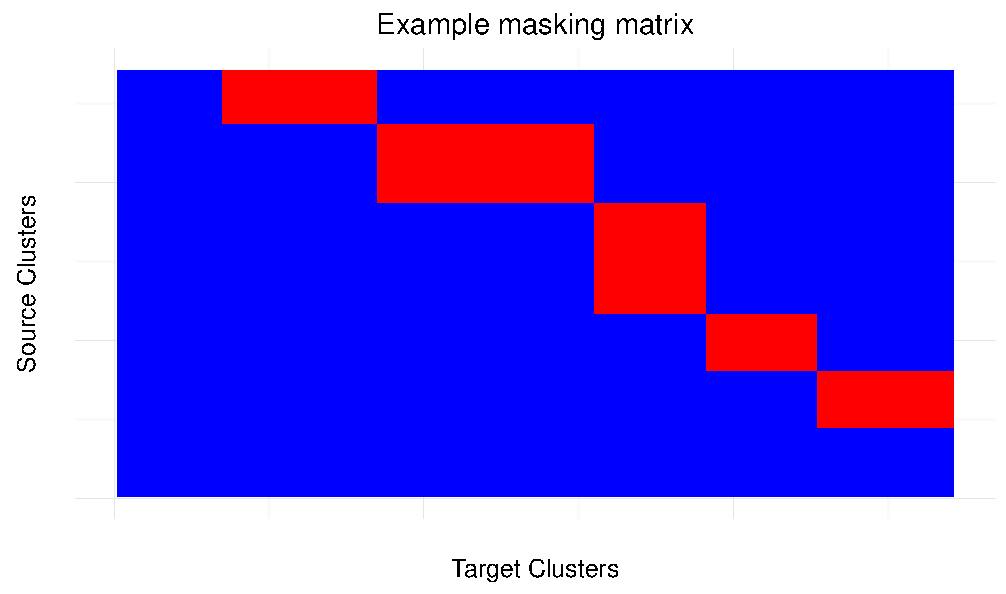
\includegraphics[width = \textwidth]{Figures/Method/ClusterMask}
    \caption[Cluster Transition Mask]{The figures shows an example mask that removes invalid Cluster transitions from the calculation of the transition matrix, note that the valid blocks sit just above the matrix diagonal. }
    \label{fig:ClusterMask}
\end{figure}

\begin{figure}[ht]
\centering
  \includestandalone{Tikz/continuationmergesplit}
  \caption[Cluster Continuation. Merge and Split]{The schematic shows a possible series of time steps where clusters $c_1$ and $c_2$ persist for three turns with little change before $c_1$ splits with most of it's nodes going to $c_2$ and the remainder forming a new node $c_3$. The arrows entering and leaving each node are nodes joining or leaving the cluster from the node soup of unattached nodes. N.B not all nodes are assigned to the two surviving clusters, some are lost to the node soup.}
  \label{fig:contmergsplit}
\end{figure}


\subsection{Node-cluster probability tables}
\label{sec:NodeClustProb}

With the Cluster families identified, creating a bi-variate conditional probability table to see the probability of a node being in a given cluster is of interest.  This is done by aggregating the matrix of Node cluster membership by cluster family so that each column represents the total number of days a node was in each of the cluster families. Dividing the rows of resulting matrix by the total row count will produce the bi-variate probability distribution. Each element of the resulting table will represent the conditional of a specific cluster given the node of interest $P(C_f|n)$, where $n$ is the node/smart meter of interest and $C_f$ is the cluster family.

\section{Analysing probability distributions}

With the creation of the transition matrix and the Node-Cluster probability table, it is instructive to see how much information can be gained from them. A simple method of doing this is to see how stable the nodes are in the clusters. For $C_f$ clusters the uniform probability of being in a cluster will be $\frac{1}{C_f}$. By squaring the elements and summing the rows, a uniform distribution will return a value of $\frac{1}{C_f}$ whilst a node that occurs in a single node only would return a value of 1. Plotting the density distribution will give a visualisation of how far from the uniform the bi-variate distribution is.

\subsection{Entropy and the KL divergence}
Although the Node stability method gives rough visual guide it can be more instructive to use the entropy of the distribution. Entropy is a measure of the uncertainty of a distribution, where a high value indicates a high uncertainty and an entropy of 0 is absolute certainty. A uniform distribution has the maximum entropy of a distribution as knowing $x$ gives zero information about the state of $y$, for a discrete distribution the entropy is always positive. Entropy itself is linked to two other concepts, the Kullback-Leibler divergence (KL-divergence) \cite{kullback1951} , and mutual information \cite{barber2012}. The KL-divergence is a measure of the similarity of two distributions and links to entropy as shown in \ref{eq:kl} where $H(p)$ is the entropy of the distribution $p$, whilst $u$ is the uniform distribution. The KL divergence is subtracted from the constant as it is always greater than or equal to zero, being zero when the two distributions are identical. The proof of that $KL(p|q)>0$ is shown in equations \ref{eq:klproofstart} to \ref{eq:klproofend}. The lowest level of useful entropy will be the marginal probability of being in a cluster i.e the probability distribution $P(C_f)$ for all values of $f$.

\begin{equation}
H(p)=-KL(p|u)+const
\label{eq:kl}
\end{equation}

 The KL divergence between 2 distributions $q(x)$ and $p(x)$ is defined as

\begin{equation}
    KL(q|p)= \left \langle log\, q(x) \right \rangle_{q(x)}-\left \langle log\, p(x) \right \rangle_{q(x)}
\label{eq:klproofstart}
\end{equation}

where $\left \langle f(x) \right \rangle$ means taking the expectation of function $f(x)$ with respect to the distribution $q(x)$.

consider the bound $log\, x \geq x-1$ show how this can be used to prove $KL(q|p)\geq0$.

\begin{equation}
    x = \frac{p(x)}{q(x)}
\end{equation}

Substitute into the bound equality
\begin{equation}
   log\,p(x)-log\,q(x) \geq \frac{p(x)}{q(x)}-1 
\end{equation}

multiply both sides by $q(x)$

\begin{equation}
    q(x)log\,p(x)-q(x)log\,q(x) \geq p(x)-q(x) 
\end{equation}

integrate both sides with respect to $x$ using the distribution property $\int q(x)dx=1 \,and \,\int p(x)dx=1 $

\begin{equation}
    \left \langle log\, q(x) \right \rangle_{q(x)}-\left \langle log\, p(x) \right \rangle_{q(x)} \geq 1-1
\end{equation}


\begin{equation}
    \left \langle log\, q(x) \right \rangle_{q(x)}-\left \langle log\, p(x) \right \rangle_{q(x)} \geq 0
\label{eq:klproofend}
\end{equation}

\subsection{Chi Squared test for independence}
A good method to test whether the two variables/axis of a  matrix are independent is to perform a Pearson $\chi^2$ independence test \cite{pearson1900}, shown. $O_i$ the number of observations of type $i$, $E_i$ is the expected frequency of type $i$ \cite{pearsonschisquaredtest2016}.

\begin{equation}
    \chi ^2 = \sum_{i=1}^n \frac{(O_i-E_i)^2}{E_i}
\end{equation}

\section{Modelling}
The main modelling approach in this project is to explore whether the method that predict the transition of nodes from one behavioural cluster to another can be used as a competitive forecasting technique when compared to a linear predictor and to see if it is in the ball park accuracy of the MAPE values obtained in the literature \ref{sec:forcesmart}, this regression model will output a single value for each half hour period that will be the prediction of the the electrical load for the whole domestic portfolio. It will be compared against a linear model that predicts using only the whole portfolio data ignoring the detail of the smart meters.

A secondary model will evaluate the ability of the transition matrix to correctly classify individual node movements instead of the en masse node flows of the main model, this classification model will predict which cluster the node will be in for the subsequent day. Whilst the comparison model of the regression will be a simple multi-linear regression, the classifier will be compared using the using the XGboost algorithm \cite{chen2016}. XGboost is a popular non-linear machine learning algorithm. The name refers to Extreme Gradient Boosting, as it is a development of earlier boosting techniques \cite{schapire2003} and boosted tree models, that were greatly popularised by Adaboost  \cite{freund1997}. However XGboost has been designed to use less resources and therefore have much greater scalability, than earlier boosting methods.

Finally a classification model will be used to take advantage of the socio-economic information available in the dataset, this model will attempt to predict socio-economic class based on electricity consumption patterns.


\subsection{Power forecasting}
The forecasting of the day ahead power will be done indirectly. A vector of the number of nodes in each cluster on day $x$ will be multiplied by the transition matrix developed in Section \ref{sec:Clusttrans} to predict the number of nodes in each cluster in day $x+1$, this will create a 1 step markov chain \cite{barber2012}. The mean node profiles of day $x$,mentioned in Section \ref{sec:LoadProfiles}, will then be multiplied by the predicted number nodes in each cluster of $x+1$, to create the predicted load profile of $x+1$. The concept with this modelling approach is that the amount of energy consumed in a domestic setting is driven by environmental factors such as temperature and light  \cite{hmgovernment2014} \cite{homesshowgreatestseasonalvariationinelectricityusetodayinenergyusenergyinformationadministrationeia2013}, as shown by the seasonal variation in Figure \ref{fig:DailyConsumption}. Therefore across neighbouring days the pattern of how and individual consumes energy would remain relatively constant but the number of people in each cluster would change based on behavioural patterns of getting home from work, evening clubs, movie night etc.
The model is defined in equations \ref{eq:begindef} to \ref{eq:enddef}, the accompanying text gives a descriptive explanation of the model and terms. for clarity a simple example using a 4 clusters and 3 time periods is show in equations \ref{eq:begineaxmple} to \ref{eq:endeaxmple}

The predicted number of nodes $\hat{N}_{x+1}$ are the product of the transition matrix $C_t$ and the number of nodes in each cluster $N_x$, where $C_t$ has dimensions $C_f \times C_f$ and $N_x$ is $C_f \times 1$ where $C_f$ is the total number of clusters.
\begin{equation}
C_t \:N_x=\hat{N}_{x+1}
\label{eq:begindef}
\end{equation}

The predicted load profile $\hat{L}_{x+1}$ is a matrix of dimensions $C_f\times t$ where $t$ is the number of time periods, in this case 12 for each half hour between 1630 and 2130, each row of the matrix represents the load profile of each cluster. $e_t$ is a vector of ones of length $1 \times t$. $\bar{L}_x$ a matrix of dimensions $C_f\times t$ where each row is the mean node load profile of each cluster on day $x$ measured in kWh. The predicted number of nodes per cluster is turned in into a matrix of dimension $C_f \times t$ by multiplying it by $e_t$, this produces a matrix where each column is the predicted nodes per cluster for day $x$ repeated $t$ times. This new matrix can then be multiplied element wise with $\bar{L}_x$ using the Hadamard product to find the predicted load per cluster.
\begin{equation}
\hat{N}_{x+1}\: e_t \circ \bar{L}_x=\hat{L}_{x+1}
\end{equation}

The total predicted load profile of $x+1$ calculated by summing the the predicted cluster loads using the vector $e_{C_f}$ which is a vector of ones of length $C_f \times 1$
\begin{equation}
e_{C_f} \:\hat{L}_{x+1}= \hat{P}_{x+1}
\end{equation}

Alternatively the above equations can be shown as a single expression. 
\begin{equation}
e_{C_f}(C_t \:N_x \: e_t \: \circ \bar{L}_x) = \hat{P}_{x+1}
\label{eq:enddef}
\end{equation}



The following equations give a simple example of how the model works using four clusters and three time periods. The three expressions represent equations \ref{eq:begindef} to \ref{eq:enddef}.

\begin{equation}
\underbrace{\begin{bmatrix}
0.5 & 0   & 0   & 0.5 \\
 0   & 0.8 & 0.2 & 0   \\
 0   & 0.2 & 0.7 & 0.1   \\
 0   & 0   & 0.1   & 0.9  \\
\end{bmatrix}
}_{Transition \; Matrix}
\underbrace{\begin{bmatrix}
200 \\ 300 \\ 100 \\ 200 
\end{bmatrix}
}_{Nodes}
=
\underbrace{\begin{bmatrix}
200 \\ 260 \\ 130 \\ 190 
\end{bmatrix}
}_{Predicted \:Nodes}
\label{eq:begineaxmple}
\end{equation}

\begin{equation}
\begin{bmatrix}
200 \\ 260 \\ 130 \\ 190 
\end{bmatrix}
\begin{bmatrix}
1 & 1  & 1 
\end{bmatrix}
\circ
\begin{bmatrix}
3 & 1 &1 \\ 
1 &4  & 1\\ 
1 & 1 &2 \\ 
 1& 3 & 4
\end{bmatrix} =
\begin{bmatrix}
600 & 200 &200 \\ 
260 &1040  & 260\\ 
130 & 130 &390 \\ 
 190& 380 & 380
\end{bmatrix}
\end{equation}

\begin{equation}
\begin{bmatrix}
 1& 1 & 1   
\end{bmatrix}
\begin{bmatrix}
300 & 100 &100 \\ 
260 &1040  & 260\\ 
150 & 150 &300 \\ 
 290& 870 & 1160
\end{bmatrix}
=
\begin{bmatrix}
1000 & 2524 &  1820 
\end{bmatrix}
\label{eq:endeaxmple}
\end{equation}



\subsection{Node cluster forecasting}

Forecasting the day ahead cluster for a specific node is done in a similar way to forecasting the load profile. Equation \ref{eq:Nodeclustforce} shows how a node prediction is made. The cluster transition matrix $C_t$ is multiplied by a cluster membership vector of node $i$ on day $x$, this vector is shown as $n^{i}_{x}$ and comes from the table described in \ref{sec:NodeClustProb}. The resulting vector is the equivalent of the output of equation \ref{eq:begindef} but for a single node. The vector is then multiplied element wise by the probability distribution of the node across clusters to adjust for the probability of the node being in each of the clusters. The argmax then finds the cluster with the highest probability and returns that as the predicted cluster for node $i$ on day $x+1$. A comparison model will be used using the XGboost model, this model will compare the performance of the transition method using the probability distributions of each node. A second XGboost model will be made that additionally takes the previous 7 days worth of cluster transitions and compares those to see if a history of transitions improves model performance.


\begin{equation}
    \underset{z\in C_f}{arg \; max}(C_t n^{i}_{x} \circ d^i)_z=P^{i}_{x+1}
\label{eq:Nodeclustforce}
\end{equation}


\subsection{Socio-demographic detection}

Finally socio-economic classification will be performed based on the probability of being in one of the given clusters, this is to test to see if electricity consumption behaviour is any indicator of social economic class, the data used will be the bi-variate probability table generated in Section \ref{sec:NodeClustProb}. The dependent variable will be the socio-economic class defined using the the Mosaic group file that is associated with each node. 


\subsection{Model Evaluation}
In order to test the efficiency of the models they will be evaluated using a variety of methods. The linear models predicting the load profile will be evaluated using RMSE, $R^2$ and $MAPE$. As they are multiclass predictors, the two classification algorithms will be evaluated using Accuracy and Cohen's kappa ($\kappa$). In the following explanations $\hat{y}$ is the predicted value and $y$ is the true value.

\begin{enumerate}
    \item RMSE: The Root Mean Square Error, a commonly used method of measuring the residual error of a regression problem, gives the result as a number larger than 0, it allows the error to be interpreted in absolute terms.
    
        \begin{equation}
            RMSE = \sqrt \frac{ \sum_{i=1}^n (\hat{y_i}-y_i)}{n}
        \end{equation}
        
    \item $R^2$: Otherwise known as the coefficient of determination this metric shows how much of the variance of the data the model explains. 
    
    \begin{equation}
        \bar{y}=\frac{1}{n}\sum_{i=1}^n y_i
    \end{equation}
    
    \begin{equation}
        SS_{res}= \sum_{i=1}^n(\hat{y_i}-y_i)^2
    \end{equation}
    
    \begin{equation}
        SS_{tot}= \sum_{i=1}^n(\bar{y_i}-y_i)^2
    \end{equation}
    
    \begin{equation}
        R^2 = 1- \frac{SS_{res}}{SS_{tot}}
    \end{equation}
    
    \item MAPE: Mean Absolute Percentage Error, compares the error in terms of the size of the true value. This is useful when the scale of the error shown by the RMSE needs contextualising, for example forecasting very small or very large numbers.
    
    \begin{equation}
        MAPE= \frac{1}{n}\sum_{i=1}^n\left | \frac{\hat{y_i}-y_i}{y_i} \right |
    \end{equation}
    
    \item Accuracy: Used for evaluating the the performance of a classifier. It is the most common and simplest form of classification performance, however it is vulnerable to skewed data distributions and so should be interpreted with care and the use of other metrics such as balanced accuracy p-value or Cohen's $\kappa$ described below. Accuracy is the total number of correct classifications, called True Positive ($T_p$) and True Negative ($T_n$)  divided by the total number of Positive ($P$) and negative ($N$) classifications.
    
    \begin{equation}
        Accuracy = \frac{T_p +T_n}{P+N}
    \end{equation}
    
    \item Cohen's $\kappa$: This metric is used for the classification problem it, shows the agreement between two sets of mutually exclusive options. The advantage of Cohen's kappa is that takes account of chance agreement and so is better able to deal with skew and the natural overlap that would be expected with random pairing. In the following equation $p_o$ is the observed agreement and $p_e$ is the agreement between the model and the truth given random performance.
    
    \begin{equation}
        \kappa = 1-\frac{1-p_o}{1-p_e}
    \end{equation}
    
\end{enumerate}

\subsection{Train and Test set}
In order to make meaningful models that are not over-fitted the data will be split into a train an test set. Generally when splitting a data set observations will be randomly sampled to ensure that there are systematic biases, that might occur if there is order within the data. The data for the classification problems will be split in this way. However the transition matrix is made by finding the intersection of the number of nodes from day $x$ and $x+1$ this means it contains data from both days arguably giving it knowledge of the surrounding data, in order to avoid creating a model which had knowledge on that which it is predicting, the transition matrix will be made useing the first 200 days and predict on the final 46. However will then risk a structural error as it has been shown in Figure \ref{fig:DailyConsumption}, that there is clear seasonal behaviour. This risk is mitigated as the movement of the nodes is being predicted using data from different seasons not the amount of power. As such creating a transition matrix in this way would only be problematic if the movement of clusters followed different patterns in summer and winter. Insight into that will be provided by the classification models.

\section{Summary}

This chapter provides detail on the method used throughout this project, providing mathematical definitions of the techniques applied and for the models developed. It discuses the checks used to ensure that the analysis provides meaningful insight into short term energy forecasting, behavioural prediction, and socio-demographic detection. The models are defined and explained for readers clarity and to improve reproducibility. 


\chapter{Results}
\label{Results}

This chapter works through the method described in section \ref{Method}, commenting on the results and providing a brief discussion of their immediate interpretation. The chapter begins with the creation of the correlation matrices, and works through to the results of the model implementation. There are 8 clusters including the catch all Soup Node, the clusters are defined by by the peak hour which is the only point the mean load profile of each cluster is significantly different from 0kWh.  The results show that the approach developed for predicting day ahead load profile using clustered smart meters, is an effective method of prediction, with a MAPE of 3.9\%, outperforming the linear predictor and having a similar MAPE score to the models used in the literature.

The classification model that predicts the cluster of each individual node produced a model whose interpretation was more mixed, it accurately predicts the correct cluster 25\% and with a low kappa score indicates that the model is not predictive. The two XGboost models the simple model with the same information and the expanded model with the previous weeks clusters performed similarly, the expanded had slightly better metric with an accuracy of  0.3689 and $\kappa$ of 0.178, which is still not very strong. Part of the reason for this poor classification performance is, that predicting in a similar time period results in a miss-classification even though the real difference is small. The low levels of consistent behaviour shown in \ref{fig:MeanAbsCorr} would suggest that predicting day ahead behaviour at node level would be challenging.  The socio-demographic detection model showed random behaviour and no predictive power this may be because it suffers from inaccuracies inherent to the MOSAIC method which is specific to an area but not a household, or simply because there is no link between socio-demographic class and electricity consumption.


\section{Creating correlation matrices} \label{sec:CormatEdge}
As there are 5260 nodes in the dataset the resulting matrix contained 2.7 million elements, of varying degree's of correlation, this structure can then be represented in a graph, the ordered correlation matrix is shown in figure \ref{fig:day100corplot}. By creating the correlation matrices for all days, it reduces the computational load for making changes later on in the processing pipeline, such as changing the minimum correlation requirements for link and rebuilding the graphs. Each correlation matrix was over 200mb matrix, together the total size of all the correlation matrices was over 40Gb.

\begin{figure}
    \centering
    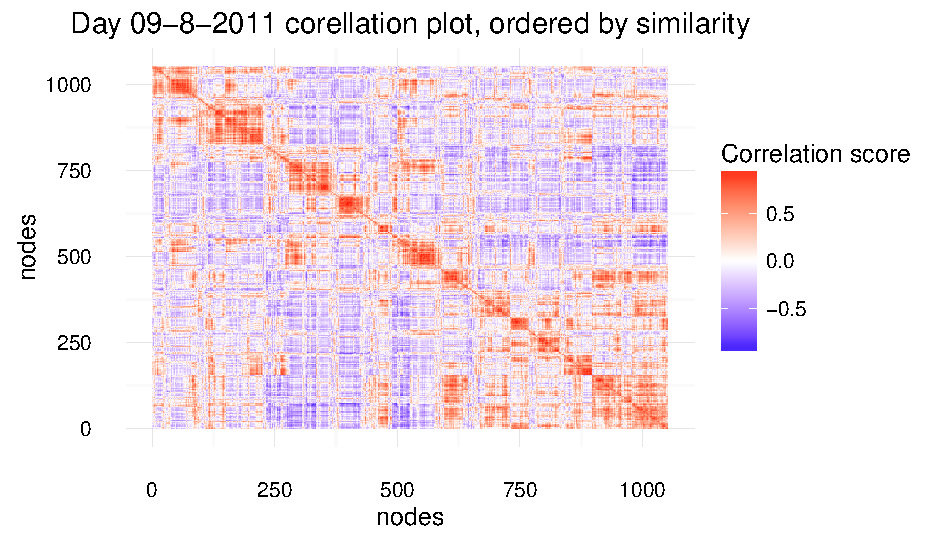
\includegraphics[width=\textwidth]{Figures/Results/day100Corplot}
    \caption[Example corellation matrix]{The correlation matrix of 09-08-2011 with the nodes organised by hierarchical similarity.}
    \label{fig:day100corplot}
\end{figure}

\section{Finding an appropriate  edge correlation cut off point}
The results of edge analysis are shown in figure \ref{fig:EdgeNodeAnalysis}. They reveal that that the number of edges and non-isolated nodes are relatively consistent across the graphs. Subfigure \ref{fig:Meanedges} shows that the number of edges decreases approximately quadratically with increasing minimum correlation. It can be seen that there is a small right skew in the data as there is a visible difference between the mean and the median, the standard deviation of the edge number is approximately 10\% of the mean. 

Sub figure \ref{fig:Meannodes} shows the mean number of nodes for each cut off point. Node number analysis showed very little variation with a negligible standard deviation and a median that is the same as the mean. It is clear that the total number of non-isolated nodes stays almost constant up to quite high levels of correlation before dropping off steeply to zero. Comparing the percentage of non-isolated nodes against the percentage of total edges as in \ref{fig:Edgenodeperc} shows that the percentage difference between the two grows quite large, figure \ref{fig:EdgeNodeDiff} shows the difference is maximised at a cut off of 0.8. 

The results of this analysis suggests that using 0.8 as a cut off will provide the highest number of non-isolated nodes for the lowest number of edges. However it should be noted that although the number of non-isolated nodes is low, experimenting with various graphs reveals that there are many nodes in small unconnected sub graphs of two or three, therefore the cut off point will be set at a more conservative 0.7. This makes a much more highly connected graph but is still tractable. 

With the cut off point chosen at 0.7 all graphs can be generated and community detection performed.

\begin{figure*}[ht]
\centering
\textbf{Number of edges analysis}\par\medskip
\subfloat[]{
  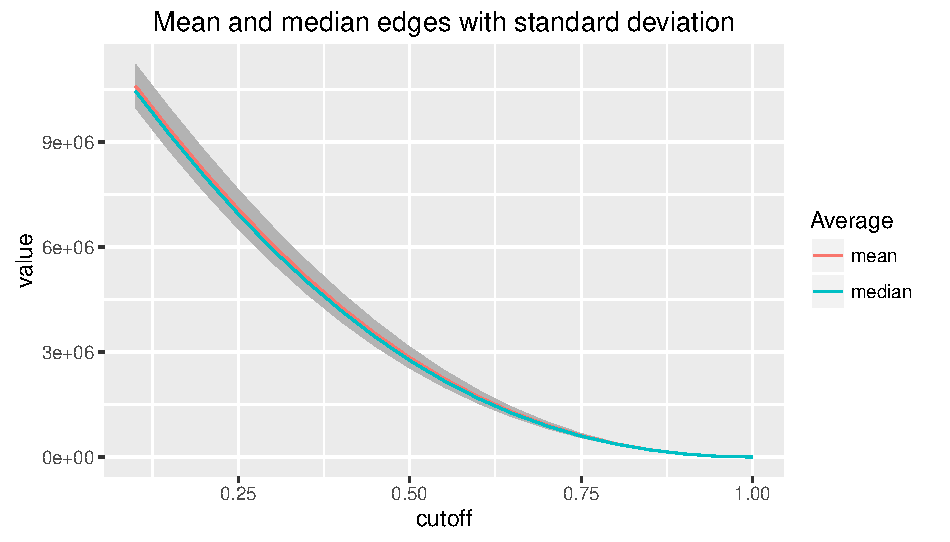
\includegraphics[width=0.49\textwidth]{Figures/Results/Meanedges}\label{fig:Meanedges}
}
\subfloat[]{
  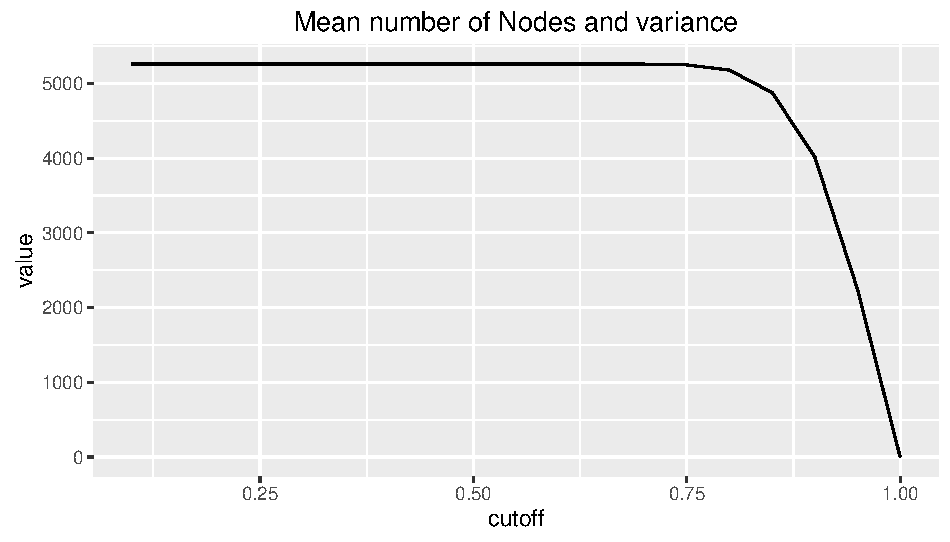
\includegraphics[width=0.49\textwidth]{Figures/Results/Meannodes}\label{fig:Meannodes}
}

\subfloat[]{
  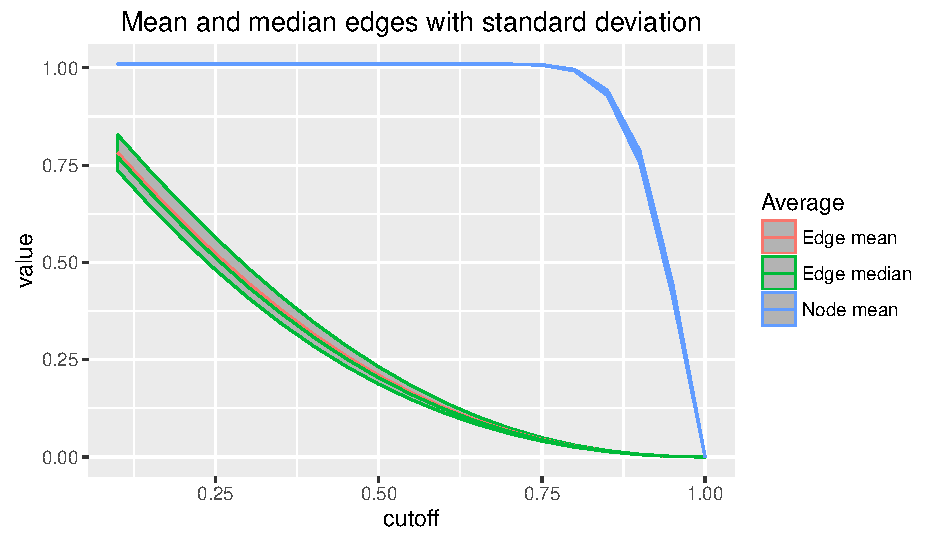
\includegraphics[width=0.49\textwidth]{Figures/Results/Edgenodeperc}\label{fig:Edgenodeperc}
}
\subfloat[]{
  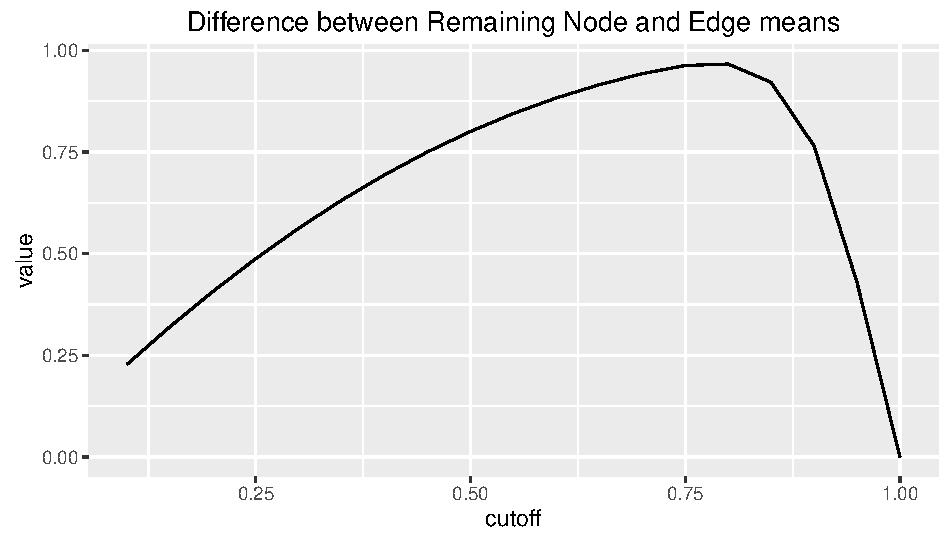
\includegraphics[width=0.49\textwidth]{Figures/Results/EdgeNodeDiff}\label{fig:EdgeNodeDiff}
}
\caption[Number of edges analysis]{Analysis of the number of edges and nodes for given correlation cut offs, across all 233 days, shows a relatively low standard deviation and slight skew with the number of edges. The number of nodes has an extremely low standard deviation, comparing the difference between the percentage remaining nodes and edges sees that the value is maximised at a correlation cut off of about 0.8. }
\label{fig:EdgeNodeAnalysis}
\end{figure*}


\subsection{Comparison with an Erdos-Renyi graph}

It is interesting to see if the the graph has a significantly different number of non-isolated nodes than an ER (Erdos-Renyi) graph for the same number of edges. This test was done by generating 20 different ER graphs with the same number of edges as the mean number of edges for each cut off point for the smart meter data. The mean number of non-isolated nodes were then compared with the mean number from the smart meter data, a plot comparing the results can be seen in \ref{fig:DataVsER}. A paired T-test was performed on the ER and smart meter non-isolated nodes. It rejected the NULL hypothesis that the mean difference between the graph types is zero with a p-value of 0.13, well above the 5\% confidence limit, there was an average difference of approximately 270 nodes. The ER graph had 0 variance for missing nodes for almost the entire test, dropping to zero on the last cut off point, this is shown in figure \ref{fig:DataVsER}. 

\begin{figure}[ht]
    \centering
    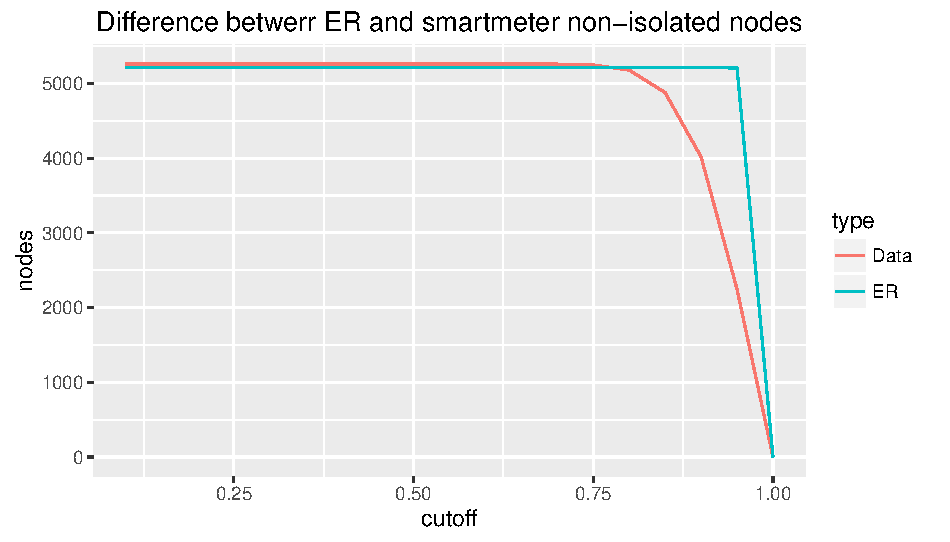
\includegraphics{Figures/Results/DataVsER}
    \caption[ER \& Data edge comparison]{There is a clear difference between the mean number of non-isolated nodes in an ER graph and the dataset. The drop-off point for the ER graph comes at some point after the 0.95 cut off.}
    \label{fig:DataVsER}
\end{figure}

\section{Creating the graphs}
Once the correlation matrices were constructed the graphs could be created, each graph was about 50Mb meaning all graphs totalled approximately 10Gb of storage space. As was seen from \ref{sec:CormatEdge} the number of edges and connected nodes drops off dramatically with a linear increase in minimum correlation requirement, this is confirmed by the graphs shown in figure \ref{fig:cutoff70vs90}, which compares a correlation requirement of 0.9 and 0.7. For ease of interpretation all unconnected nodes have been removed from the image. Figure \ref{fig:day100-90} has considerably fewer nodes than \ref{fig:day100-70} and is in comparison sparsely connected, the result is that the two images look entirely unrelated when they are in fact based on the same day with only a 0.2 change in correlation requirement. 

Another point of interest in the image is to see how communities are located within the graph as figure \ref{fig:day100-90} is much more sparse it is easier to see how the nodes are related to each other. It can be seen that clusters can form where nodes can be more related to a neighbouring cluster than to far away members of their own cluster. Ideally all cluster members are highly connected to the other members of their cluster and less to nodes outside the cluster, however as seen in the figure this may not always be the case. Cluster shape and spread is linked to modularity as described in \ref{chap:creategraph}, and graphs such as \ref{fig:day100-90} where the clusters were detected using the computationally cheap Fast-Greedy algorithm, may be expected to have quite a low modularity. This is why choosing the community detection algorithm in the next step is so important.

\begin{figure*}[ht]
\centering
\textbf{Example graphs with different cut offs}\par\medskip
\subfloat[]{
  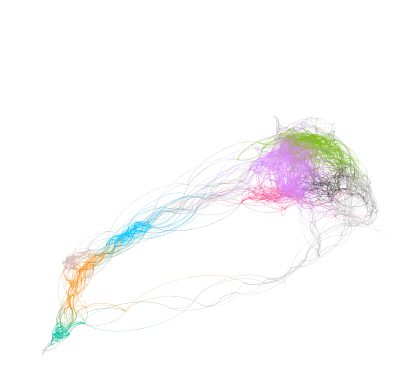
\includegraphics[width=70mm]{Figures/Results/day100-90}\label{fig:day100-90}
}
\subfloat[]{
  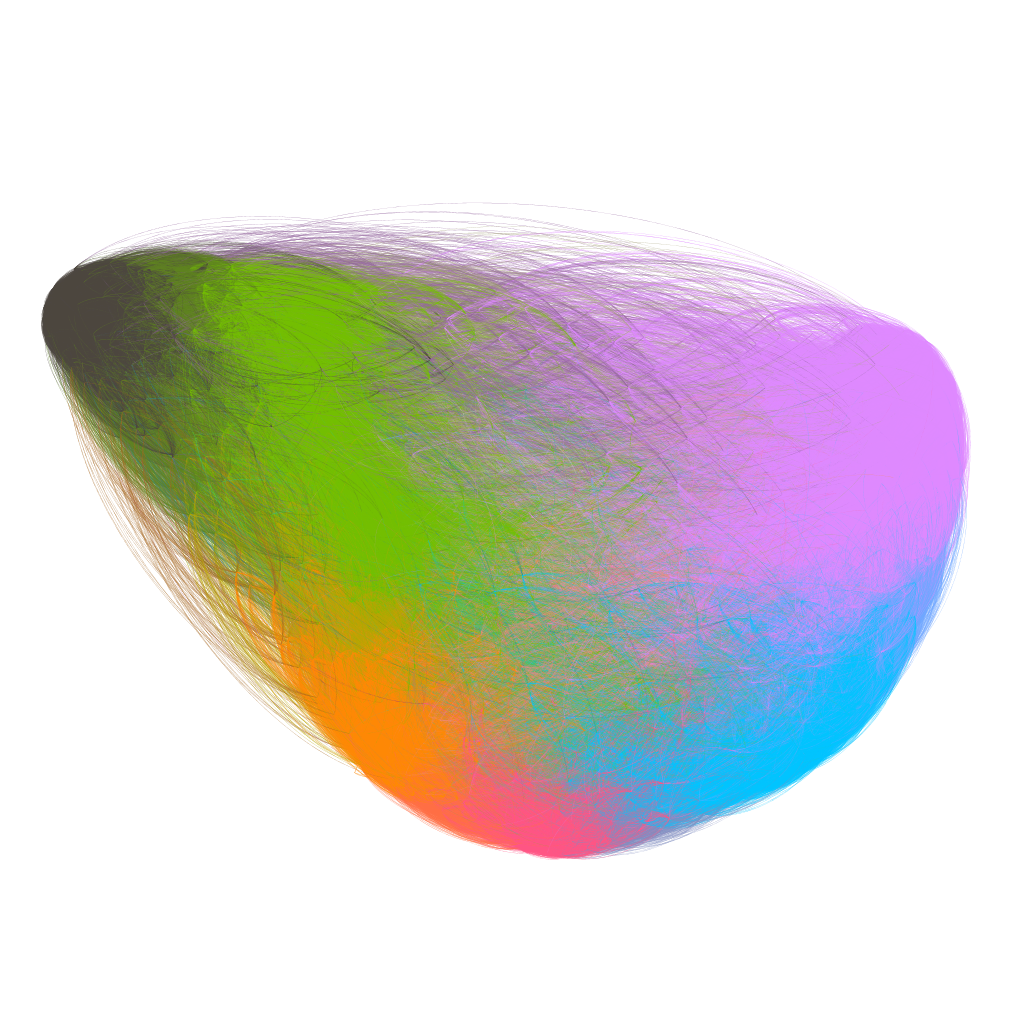
\includegraphics[width=70mm]{Figures/Results/day100-70}\label{fig:day100-70}
}

\caption[Example graphs with different cut offs]{Example of day 09-08-2011 with different correlation cut offs, nodes have been removed for ease of viewing, but edges are coloured by cluster. The difference between graphs with different cut off points can be dramatic. Figure \ref{fig:day100-90} has a cut off point of a minimum correlation of 0.9 whilst \ref{fig:day100-70} has a cut off of 0.7. As can be seen the number of edges is much higher. Clusters were detected using the Fast-Greedy algorithm.}
\label{fig:cutoff70vs90}
\end{figure*}


\section{Labelling clusters}
\label{sec:labelling}
Once all the day graphs had been made and the day labels assigned there were over 2000 total clusters. In order to get an overview of cluster behaviour the total number of clusters each day were plotted in figure \ref{fig:Total_Clusters}. The figure shows that the rolling mean number of clusters stays more or less stable at the total mean of 25.5 for all clusters and 9.4 for the large clusters. However the standard deviation is relatively large at 7.3 for the total clusters and 2.4 for the large clusters, what's more the standard deviation increases towards the end of the period, although this could be due to the onset of winter which tends to increase behaviour variation in energy use (as shown in figure \ref{fig:DailyConsumption}). In order to get a more detailed view of the behaviour of clusters a simple labelling regime was used by ranking each cluster in order of size and assigning a label to each cluster according to rank that day. This method produced figure \ref{fig:clustrank}, which shows high levels of variation from period to period in clusters of the same rank. This is understandable in the context of the the previous figure as intuitively as the number of clusters vary the size of the clusters will also vary with some inverse relation as the total number of available nodes stays constant.

\begin{figure*}[ht]
\centering
\subfloat[]{
  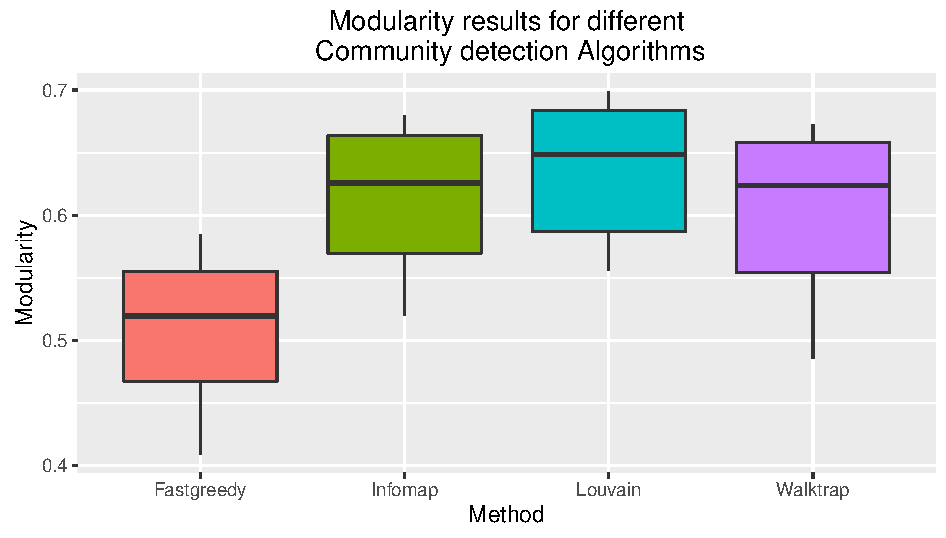
\includegraphics[width=0.80\textwidth]{Figures/Results/CommModComp}\label{fig:CommModComp}
}

\subfloat[]{
  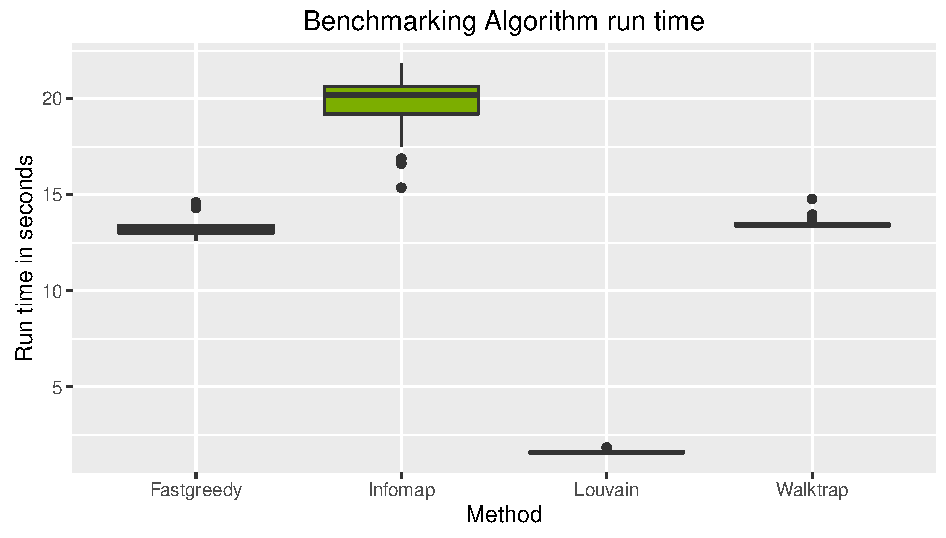
\includegraphics[width=0.80\textwidth]{Figures/Results/AlgorithmTimes}\label{fig:Algtime}
}

\caption[Cluster Family Load Profiles]{ Benchmarking the four target algorithms, shows that Walktrap, Infomap, and Louvain are all statistically similar in performance with Louvain getting slightly better results, however Louvain is considerably faster when it comes to detecting clusters}
\label{fig:ChooseAlg}
\end{figure*}



\begin{figure}[ht]
    \centering
    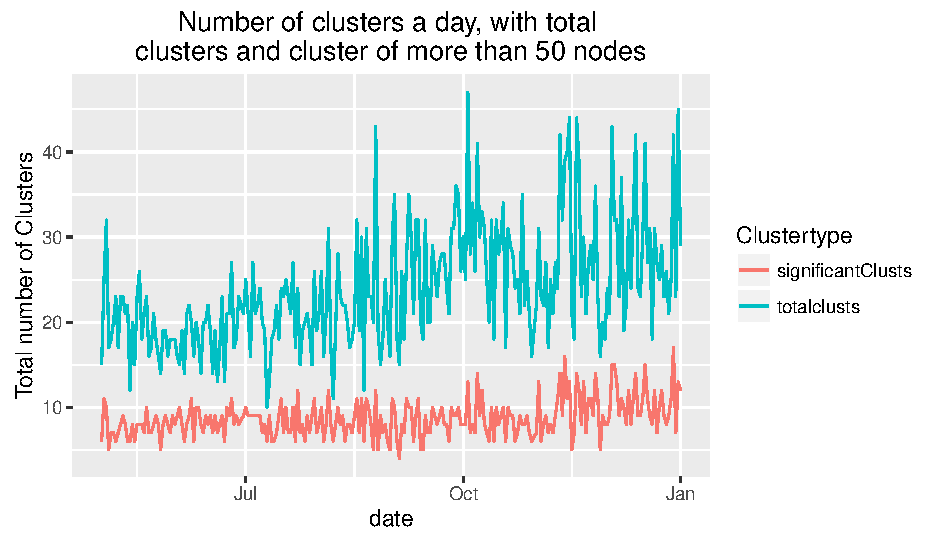
\includegraphics[width=\textwidth]{Figures/Results/TotalClusters}
    \caption[Total clusters over time]{The total number of clusters or communities detected over time has quite a large amount of variation. Although it can be seen that there are many clusters that are insignificant even the significant clusters have quite large variation }
    \label{fig:Total_Clusters}
\end{figure}

\begin{figure}[ht]
    \centering
    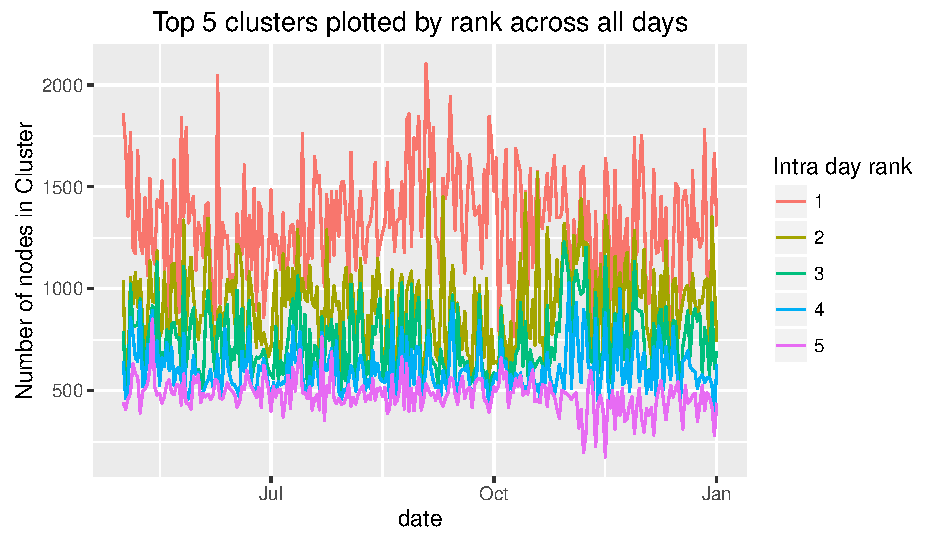
\includegraphics[width=\textwidth]{Figures/Results/Clusterrank}
    \caption[Size comparison of the largest clusters]{The total number of nodes in each cluster larger than 50. The cluster ID's are assigned by size rank. The results are interesting as there is a large amount of noise in the cluster sizes which do not hold steady throughout the period.}
    \label{fig:clustrank}
\end{figure}
\FloatBarrier 

Using the labelling method described in \ref{sec:labelClust}, the inter-cluster correlation matrix was created using clusters that had a at least 50 nodes (see fig \ref{fig:corheat}). This was then turned into a graph and communities detected using the same method as for the original graphs and community detection, but with a cut off of 0.85 instead of 0.7 as there was much more consistency in the cluster correlations. The resulting graph and communities can be seen in figure \ref{fig:DragonPlot}. These clusters can be classified into time periods as shown in \ref{fig:Familypattern}. The soup family of clusters is for clusters that are either less than 50 nodes and so are not large enough to give reasonable results, or are a cluster that is less than 1\% of the total volume of nodes in the whole 246 day period. An interesting effect on \ref{fig:DragonPlot} is that the clusters are mostly connected only within cluster and between temporarily adjacent clusters. This is because they are inherently more highly correlated with nearby clusters than ones that are further away. The clusters at the later part of the evening, specifically the 2000 and 2100 clusters, can be seen to be made up of a group of subclusters which is seen by the bumpiness in figure \ref{fig:DragonPlot}. It can also be seen more explicitly in \ref{fig:ClusterFamilySample} where both cluster 1600 and 2100 can be seen to have two peaks, whilst the 1800 cluster has got variance but had only a single peak. Figure \ref{fig:AllNodesClustercolour} in the appendix shows the compound plots of the clusters that make up each cluster family, Figure \ref{fig:AllCLustFamilies} plots all the clusters showing the separation of each cluster and the areas of overlap.

The final clusters were 1630, 1700, 1730, 1800, 1830, 1900, 2000, and the node Soup. Figure \ref{fig:Familypattern} shows how consistent these forms are using mean, median, and sum although the form breaks down somewhat on the plot of standard deviation.


\iffalse
A more consistent method of assigning labels is to use Jaccard similarity. This was calculated using the vector of nodes in each cluster as the similarity measure, this then allowed a new graph to be made and communities within that to be detected. Figure xxx shows that there is very high similarity within clusters and very low levels of similarity between clusters, suggesting that there is very little overlap between clusters in terms of nodes and that nodes seldom move between different cluster groups. One of the things that is important to consider when using Jaccard clustering is that it will create communities based on which smart meter is in each cluster not on how electricity is being consumed.
\fi

\begin{figure}[ht]
    \centering
    \textbf{Relationship between cluster families}\par\medskip
    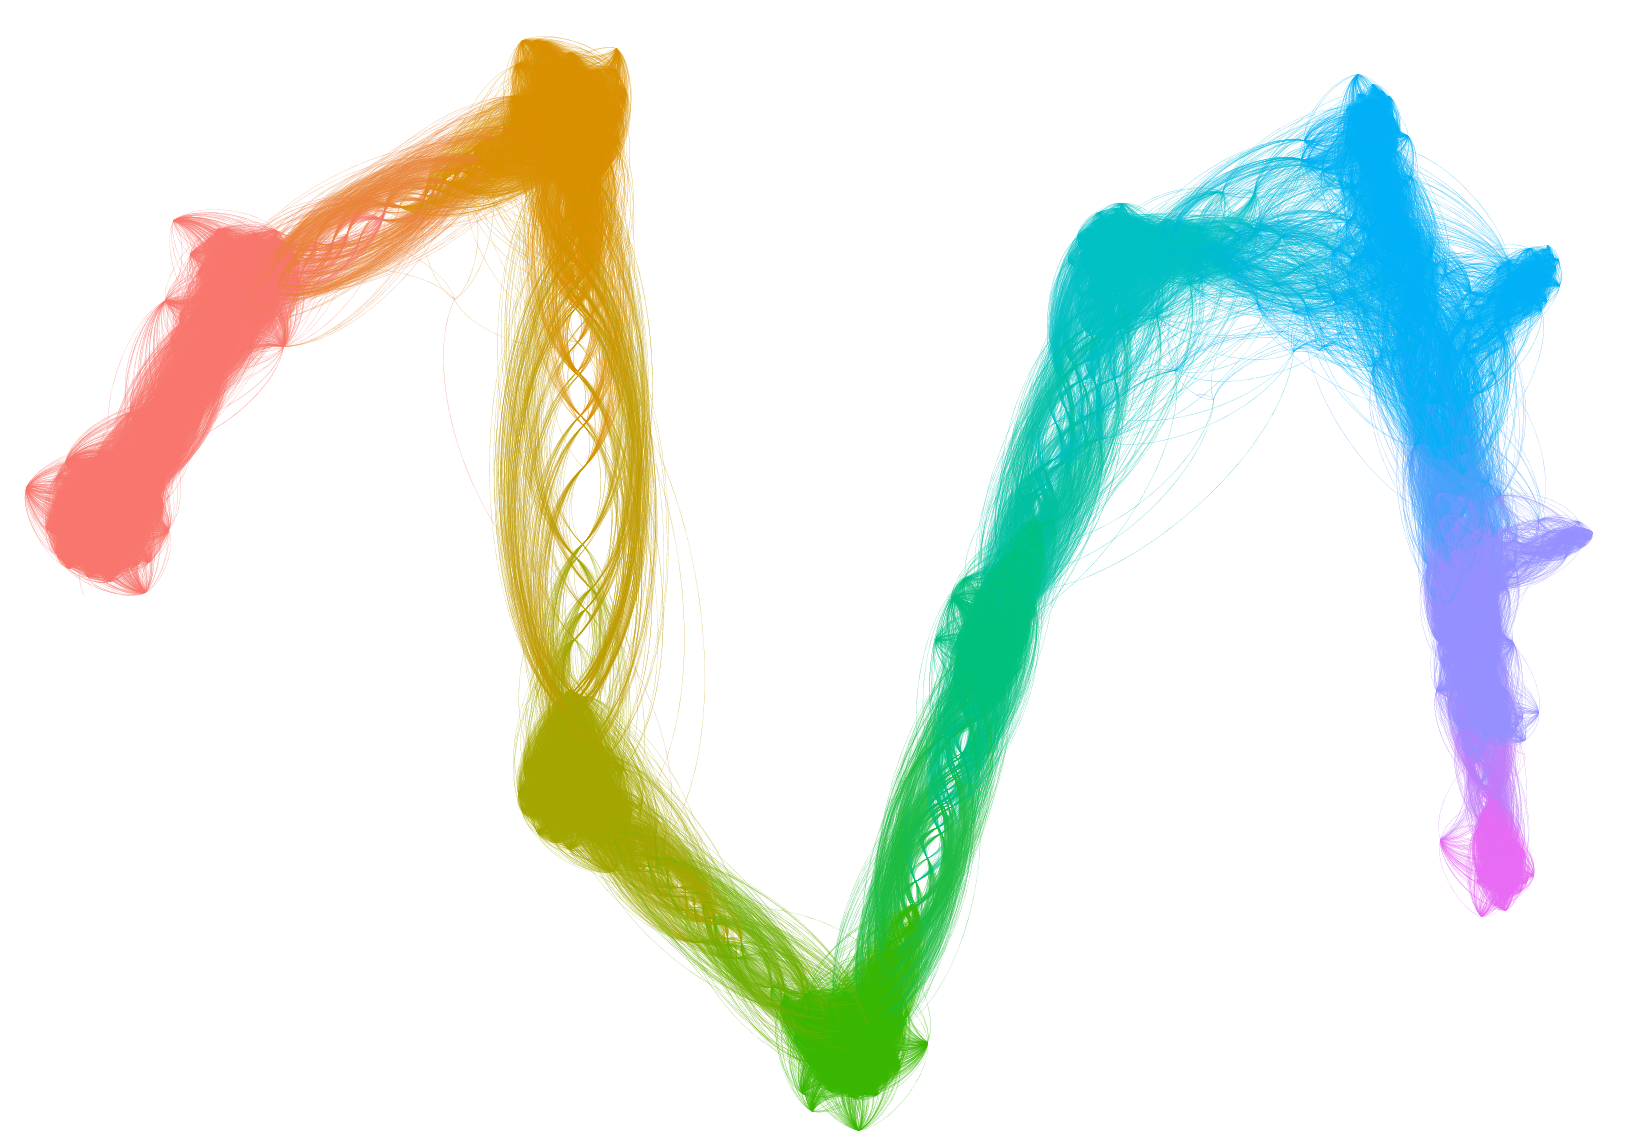
\includegraphics[width=\textwidth]{Figures/Results/Dragon}
    \caption[Cluster family Graph]{The Clusters were grouped into cluster families, each family represented a peak at a specific time of the evening, the figure shows these families, moving from the 1600 cluster on the left to the 2130 cluster on the right.}
    \label{fig:DragonPlot}
\end{figure}


\begin{figure*}[ht]
\centering
\subfloat[]{
  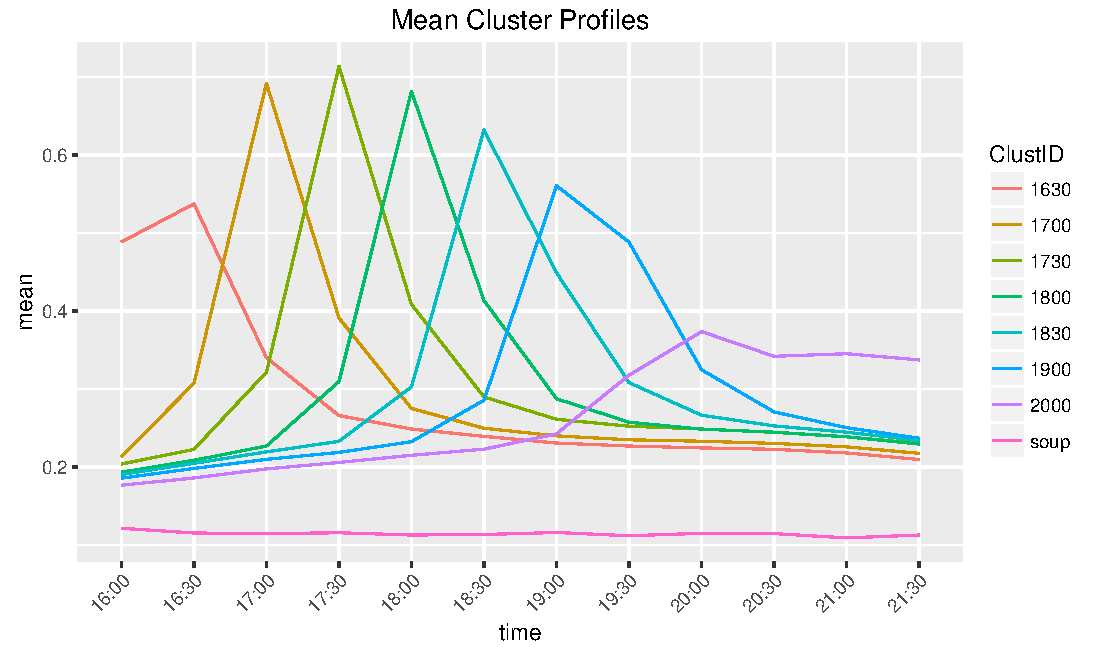
\includegraphics[width=0.49\textwidth]{Figures/Results/ProfileMean}\label{fig:Clusmean}
}
\subfloat[]{
  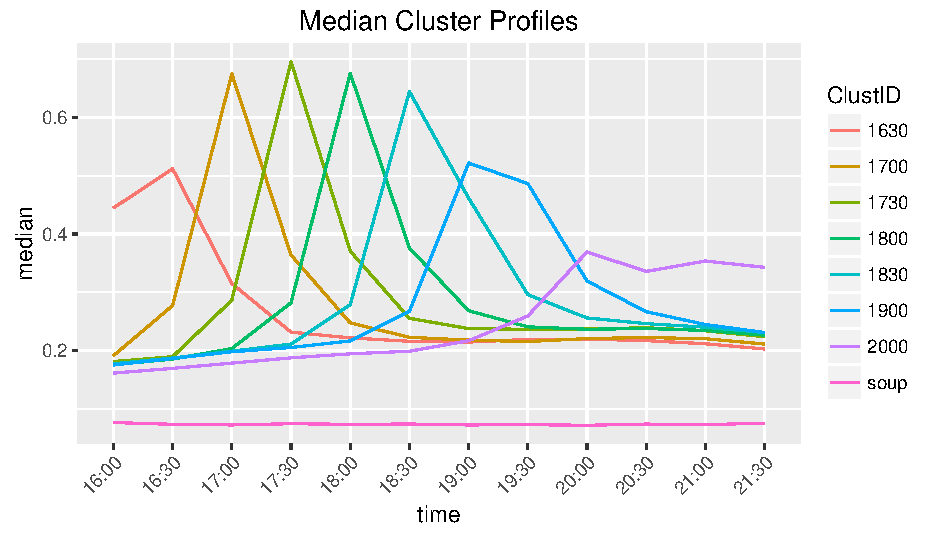
\includegraphics[width=0.49\textwidth]{Figures/Results/ProfileMedian}\label{fig:Clusmedian}
}

\subfloat[]{
  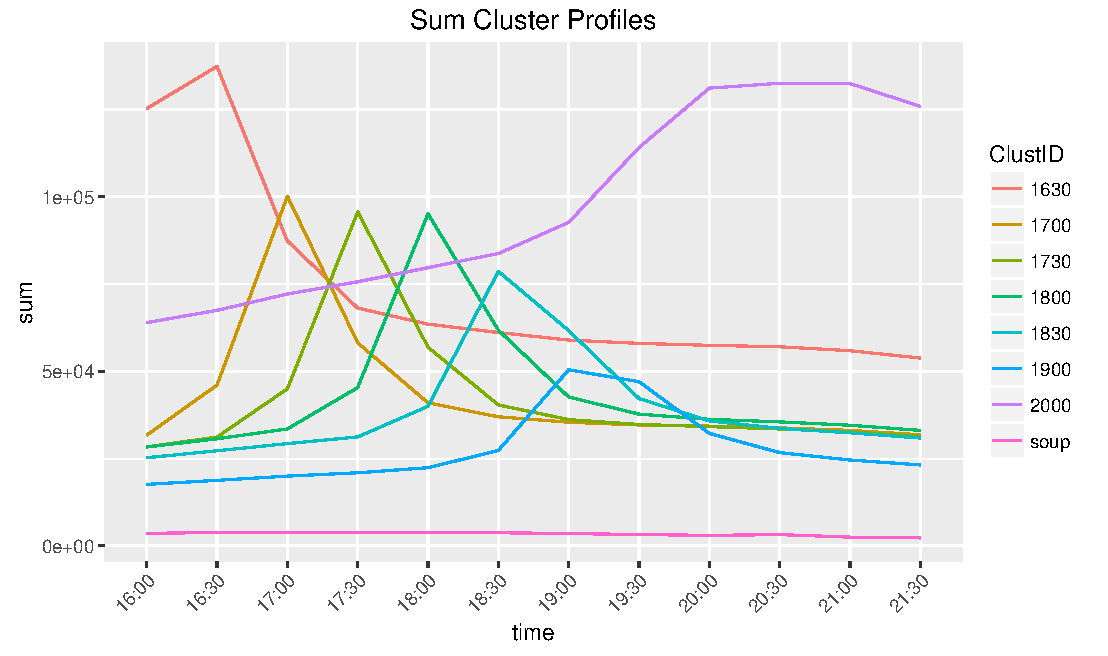
\includegraphics[width=0.49\textwidth]{Figures/Results/ProfileSum}\label{fig:CLussum}
}
\subfloat[]{
 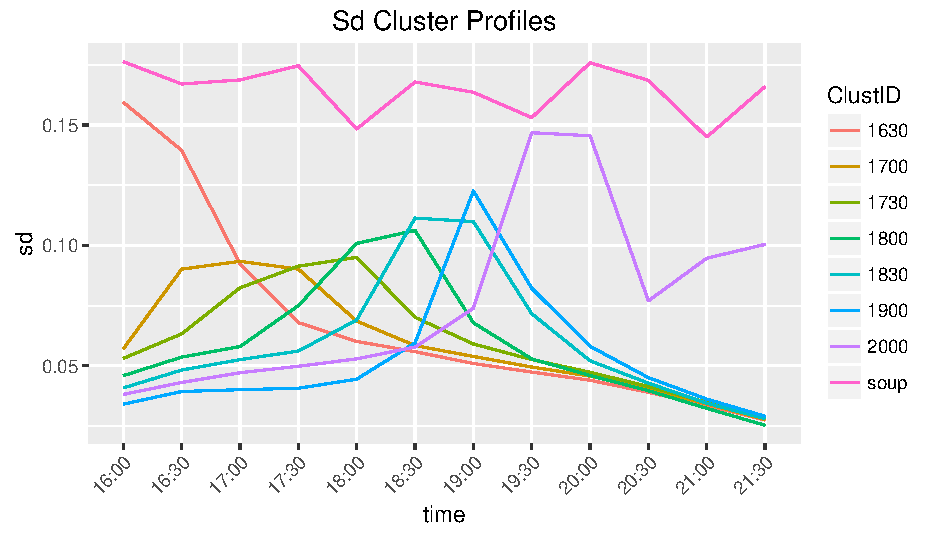
\includegraphics[width=0.49\textwidth]{Figures/Results/ProfileSd}\label{fig:Clusvar}
}
\caption[Cluster Family Load Profiles]{This series of figures is similar to \ref{fig:daypattern}, except instead of showing the day load profile, it shows the load profile for the cluster families overall. As can be seen in \ref{fig:Clusvar} variance is considerably lower than in \ref{fig:dayvar}, this is because the clustering causes an information loss smoothing the final result and reducing aggregate results.}
\label{fig:Familypattern}
\end{figure*}


\begin{figure}[ht]
    \centering
    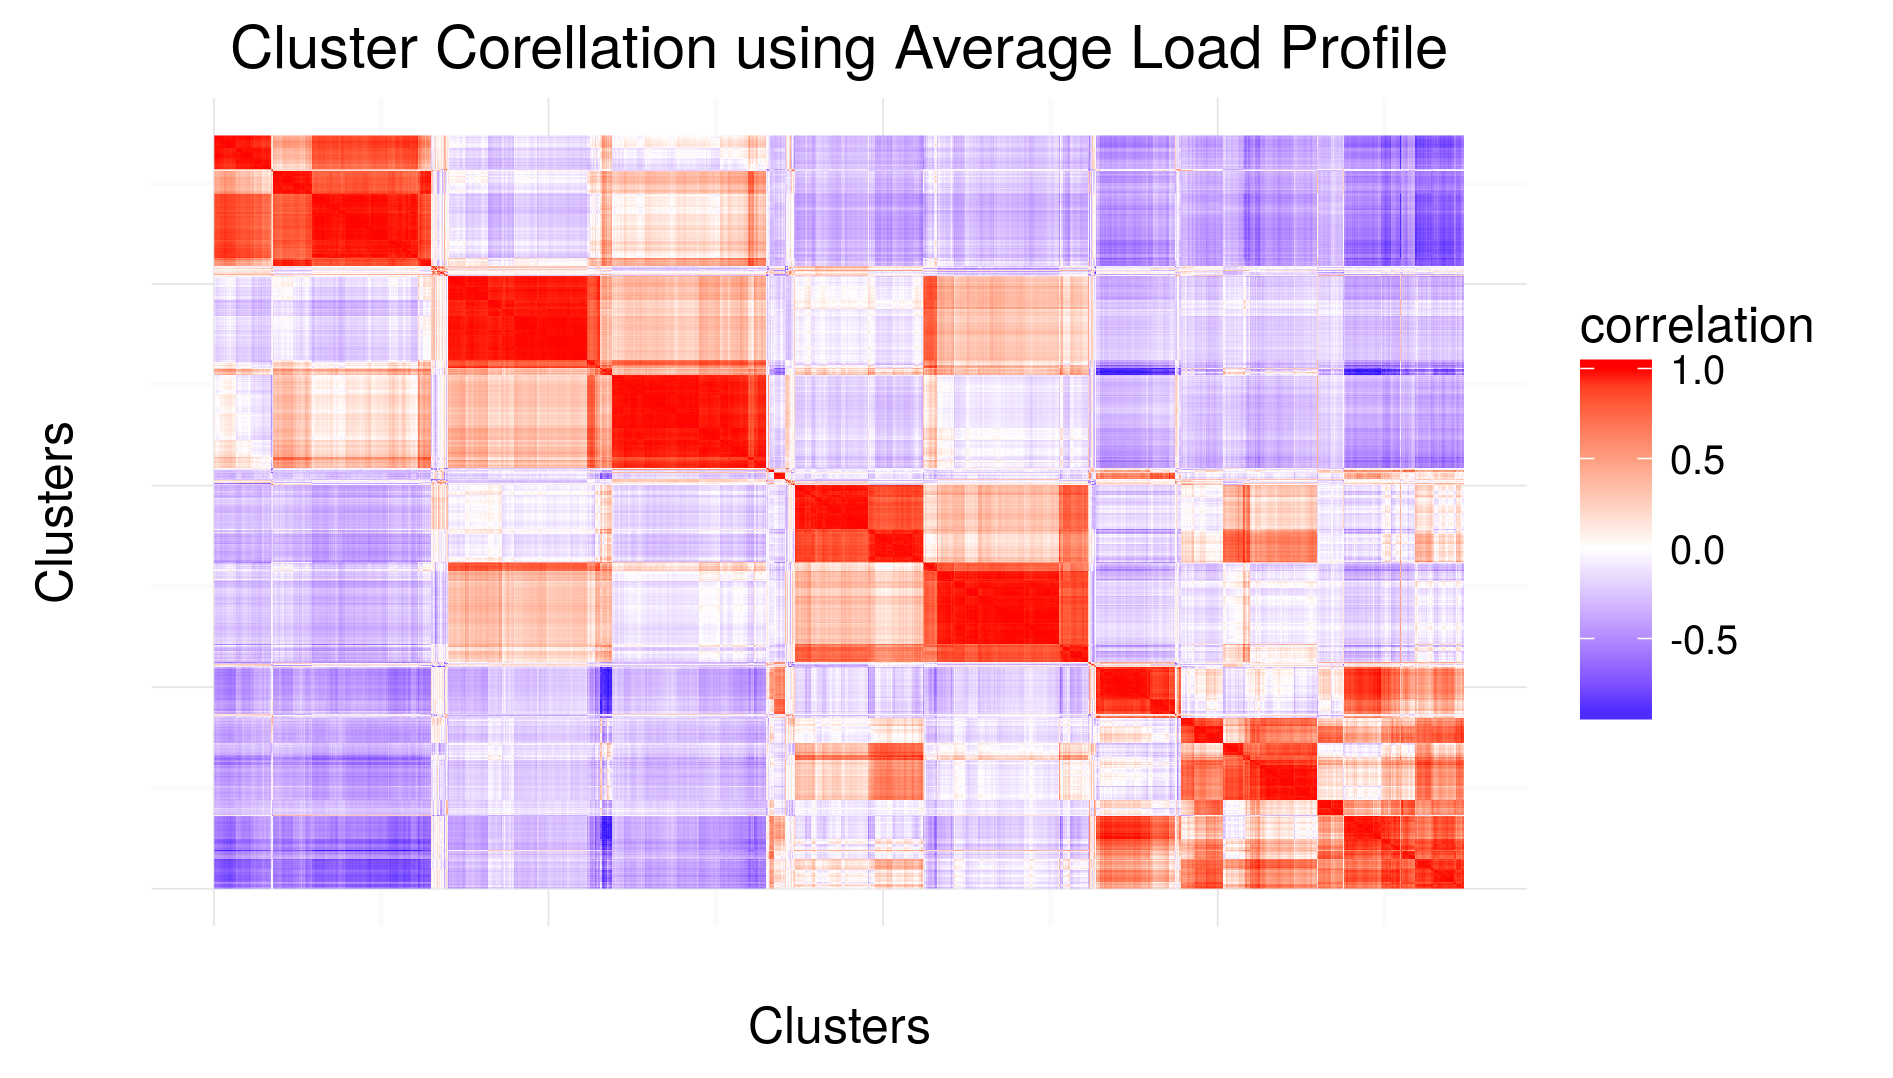
\includegraphics[width=\textwidth]{Figures/Results/ClusterCorLoadLarge.png}
    \caption[Cluster similarity heatmap]{The heat map of Cluster similarity shows that there are very low levels of cross cluster similarity and very high levels of within cluster similarity. The modularity of these communities was 0.83}
    \label{fig:corheat}
\end{figure}

\begin{figure}
    \centering
    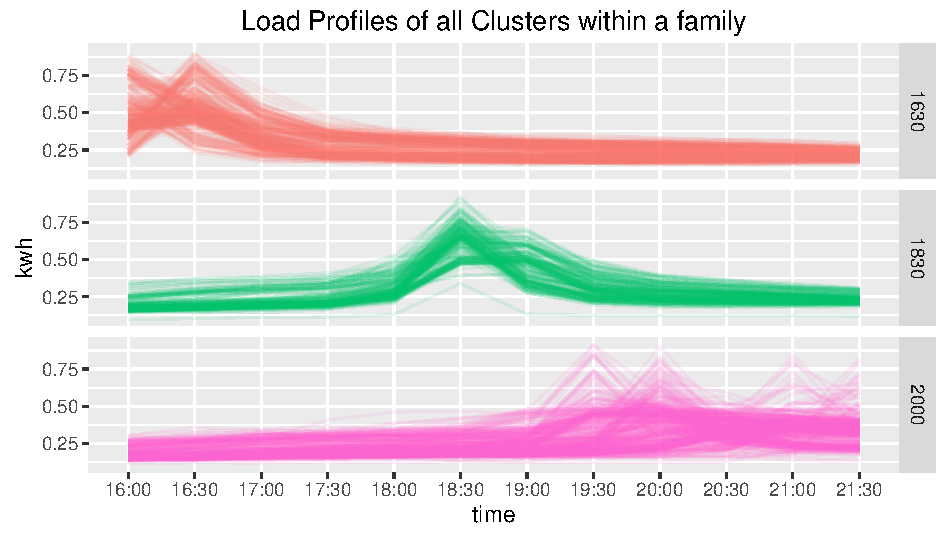
\includegraphics[width=\textwidth]{Figures/Results/ClusterFamilySample}
    \caption[Within Cluster Family Node Profile]{The figure shows all the clusters from the same family layered on the same plot.}
    \label{fig:ClusterFamilySample}
\end{figure}


After the cluster families had been decided, it was important to see how frequently each of the cluster families occurred across the time period. Figure \ref{fig:Clusterocurrance} shows red if the cluster is present and blue if the cluster is not present. Only cluster 1630 is present on all days cluster 1700, 2000 and the soup are present on most days, the 1900 cluster can be especially sparse a fact that causes prediction problems in \ref{fig:BoxTimeErr}. It's interesting consider that the node soup does not occur everyday, this means that on some days there are no nodes with significantly different behaviours. Missing clusters is most likely a side effect of using non-overlapping clustering algorithms and hard clustering nodes into only 1 cluster. 
Figure \ref{fig:SankeyWeek} shows a Sankey or Alluvial diagram \cite{sankeydiagrams} \cite{rosvall2010} which visualises flow and thus can be used to represent change in network structure. The Sankey diagram shows the volume of flow between clusters across days and it is possible to see days when clusters are missing in this case day 4 (07-08-2011) is missing the 1730 cluster. As can be seen the clusters all transition to each other to some degree, this makes the sudden disappearance of a cluster seem and unrealistic reflection of behaviour patterns and more an artifact of the clustering process. Looking at the Sankey diagram it can seem like the transitions are simply proportional to the size of the cluster however the $\chi ^2$ test of the transition matrix and node distribution in \hl{XXX} show that there is in fact a structure to the movement.

\begin{figure}
    \centering
    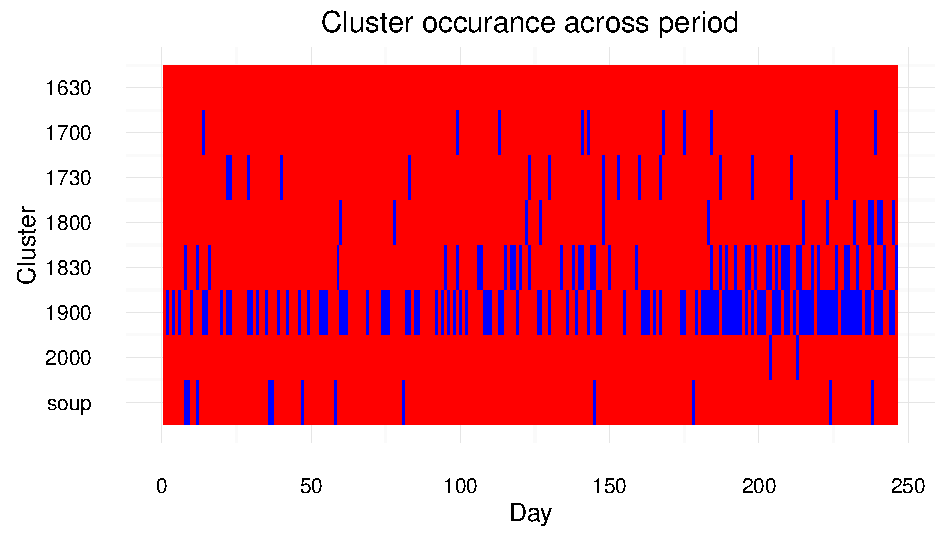
\includegraphics[width=\textwidth]{Figures/Results/Clusterocurrance}
    \caption[Cluster Occurance]{The occurrence of each cluster family across all days. As each node is clustered exclusively into a single cluster each day, it can happen that some days not all clusters are present. This doesn't mean that there were no nodes peaking at that time but is more an artifact of using non-overlapping clustering algorithms.}
    \label{fig:Clusterocurrance}
\end{figure}


\begin{figure}[ht]
    \centering
    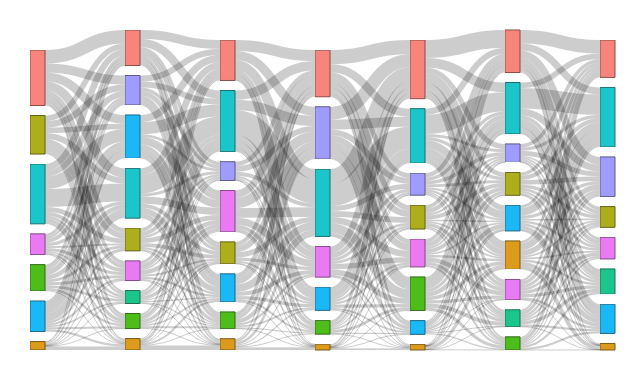
\includegraphics[width=\textwidth]{Figures/Results/SankeyWeek.png}
    \caption[Sankey diagram for 1 week]{Sankey Diagram showing the week including Saturday 09-08-2011 which is the $6^{th}$ day/layer of the Sankey Diagram, the colour scheme is the consistent with the Cluster labels elsewhere in this work, e.g the node soup shown in red. The order of the clusters in each day are optimised to reduce cross over, however as can be seen there is a lot of cross cluster movement of nodes between days, this reflect the probability of transfer seen in the transition matrix. }
    \label{fig:SankeyWeek}
\end{figure}


\subsection{Looking at cluster load profiles for a single day}

As a control, looking at an individual days load profile is instructive. Using 09-08-2011 as an example figure \ref{fig:daypattern} shows the load profiles of each cluster, table \ref{table:NodesPerCluster}, gives the nodes per cluster. The figure shows that each cluster exhibits a clear and distinct load profile across each metric similar to the cluster families in figure \ref{fig:Familypattern}. What is surprising is that the standard deviation of the profiles also reflects the over all profile pattern, to a much higher degree than in the plot of the cluster families, This is because the smoothing effect of the clustering has not been applied and so there is more natural variation possible than in the aggregated values of the clusters.

\begin{figure*}[ht]
\centering
\textbf{Day Load Profiles for 09-08-2011}\par\medskip
\subfloat[]{
  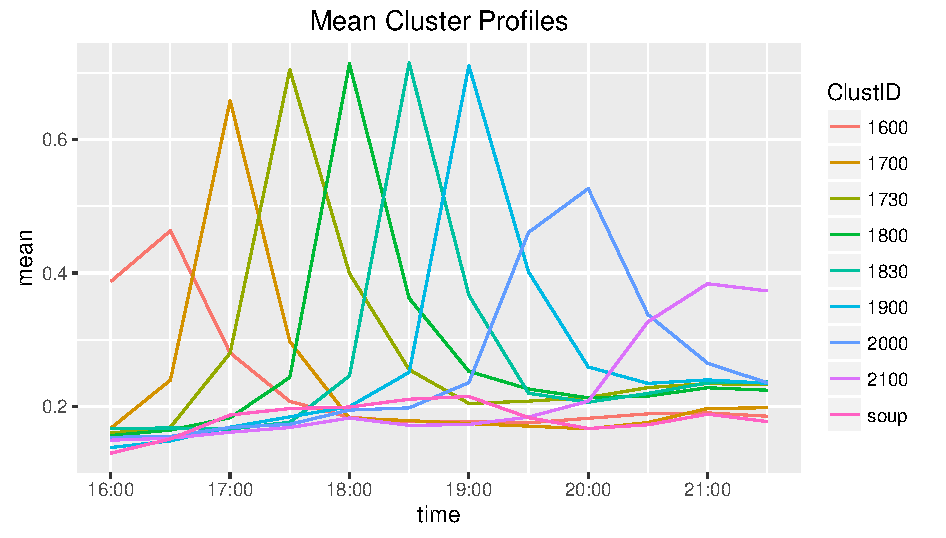
\includegraphics[width=0.49\textwidth]{Figures/Results/singledaypatternMean}\label{fig:daymean}
}
\subfloat[]{
  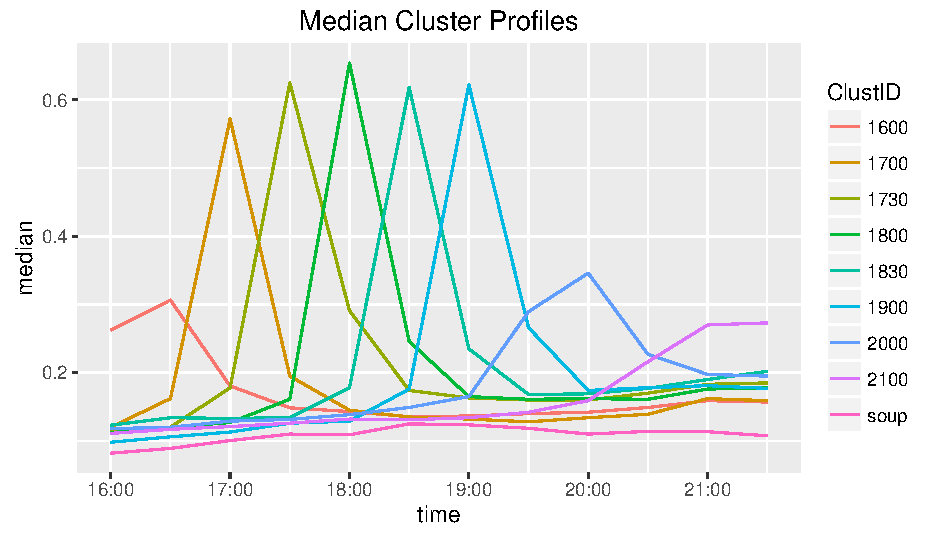
\includegraphics[width=0.49\textwidth]{Figures/Results/singledaypatternMedian}\label{fig:daymedian}
}

\subfloat[]{
  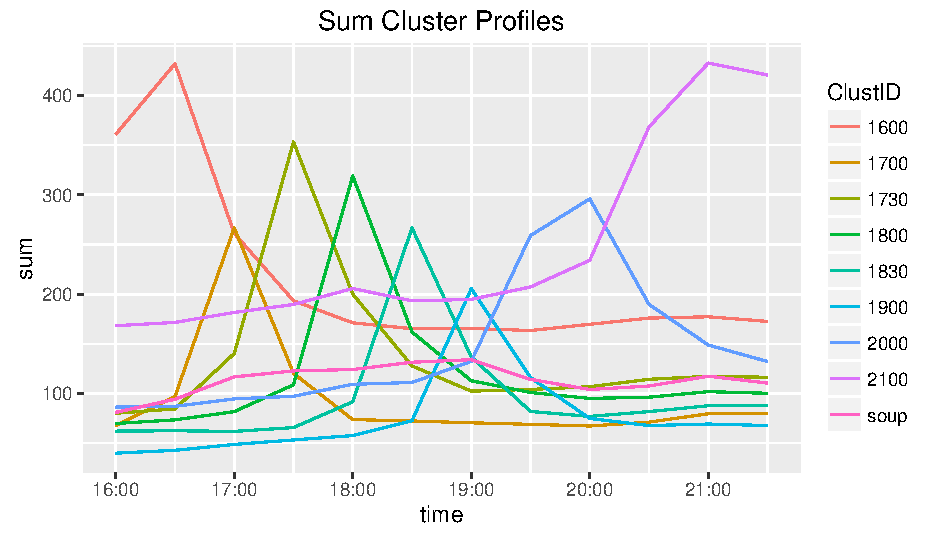
\includegraphics[width=0.49\textwidth]{Figures/Results/singledaypatternSum}\label{fig:daysum}
}
\subfloat[]{
 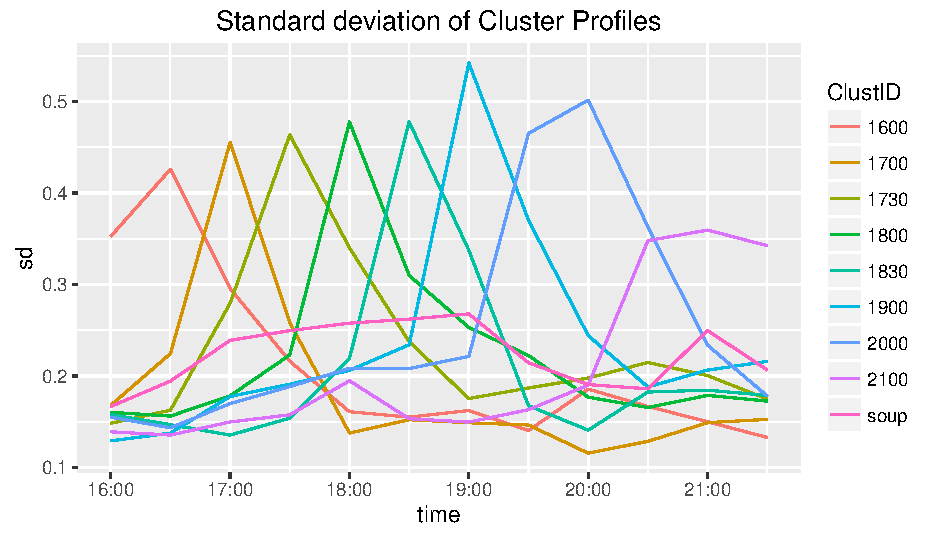
\includegraphics[width=0.49\textwidth]{Figures/Results/singledaypatternVar}\label{fig:dayvar}
}
\caption[Day Load Profiles for 09-08-2011]{This series of figures shows the pattern for day 09-08-2011 with a .7 cut off using walktrap clustering}
\label{fig:daypattern}
\end{figure*}


% latex table generated in R 3.3.0 by xtable 1.8-2 package
% Wed Aug 17 16:14:55 2016
\begin{table}[ht]
\centering
\begin{tabular}{rlr}
  \hline
 & ClustID & count \\ 
  \hline
1 & 1630 & 946 \\ 
  2 & 1700 & 508 \\ 
  3 & 1730 & 546 \\ 
  4 & 1800 & 520 \\ 
  5 & 1830 & 406 \\ 
  6 & 1900 & 657 \\ 
  7 & 2000 & 1604 \\ 
  8 & soup &  73 \\ 
   \hline
\end{tabular}
\caption[Nodes per cluster]{The total number of nodes in in each cluster for 09-08-2011} 
\label{table:NodesPerCluster}
\end{table}



\begin{figure}
    \centering
    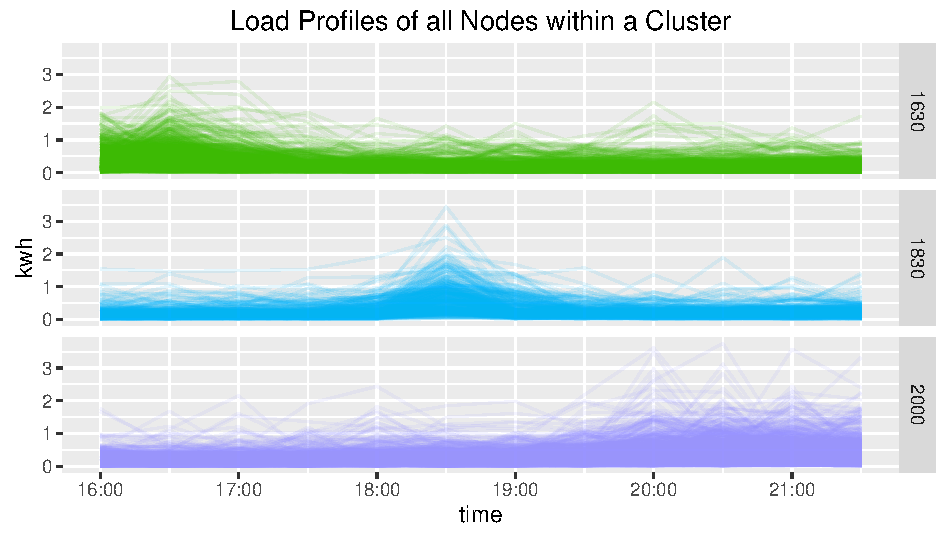
\includegraphics[width=\textwidth]{Figures/Results/NodeProfilesInCluster}
    \caption[Within Cluster Node Profile]{The within Cluster Node Profile show that although there is a lot of noise the nodes generally have their peaks at similar times. It is worth remembering that the edges and weights were decided by using a Spearman correlation which takes the rank similarity not the similarity itself.}
    \label{fig:NodeProfilesInCluster}
\end{figure}


\section{Analysing probability distributions}

After the clusters had been divided into families and their behaviour classified it was interesting to explore how the clusters and nodes interacted. Figure \ref{fig:TransitionHeat} shows a heat map of the transition matrix (the table of probabilities can be seen in \ref{tab:clustrans}). This heat map shows the probability of a node transitioning from cluster A to cluster B on consecutive days. Although there is no extremely high probability of transfer on the table it can be seen that there is a higher probability of transitioning to the same cluster than other clusters. Cluster 1600 and cluster 2100 have the highest probability of being transferred to from other clusters. 
Along with the Soup, clusters 1600 and 2100, also have the highest probability that nodes will stay within the cluster across days and not transfer out.
These insights are interesting as it implies that certain nodes consistently follow patterns that are not in any of the main clusters and so are more likely to remain in the soup. Also that people tend towards the 1600 and 2100 nodes despite the fact that they are at different ends of the evening. It's interesting to reflect why the 1600 and 2100 nodes are so popular, 
One reason may be that in the UK schools finish at 1530 and so the 1600 cluster reflects the time that children get home, in this circumstance it there would be a large group of people who would usually get back at the same time. This would explain the higher transfer probability and also the relatively large size of the 1600 group. The 2100 group could be professionals without children who have been working late or have spent the early part of the evening out before returning home. An alternative idea for the 2100 group is that it is an artifact of the simplifying of the clustering process and that people are active at other parts of the evening but that this time is peak TV watching and so many people are being clustered there due to television watching habits.


\begin{figure}[ht]
    \centering
    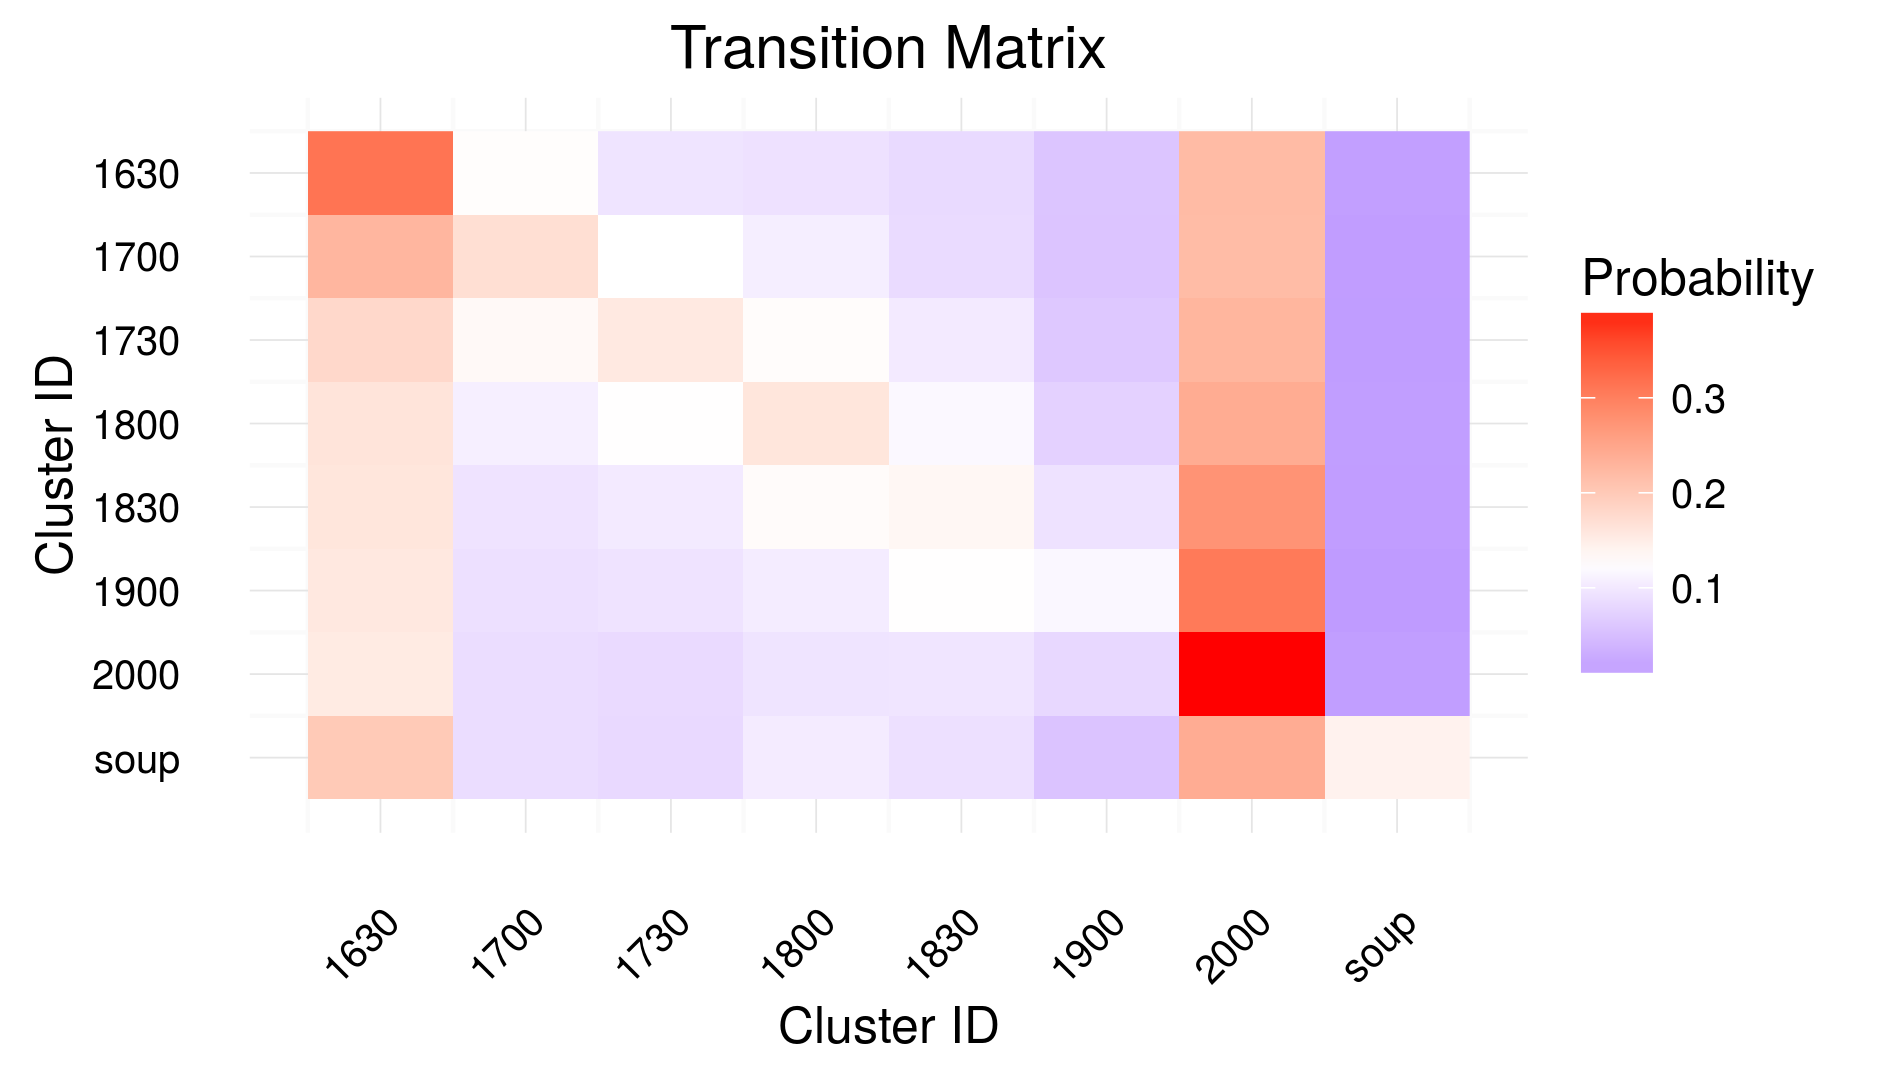
\includegraphics{Figures/Results/Clusttransgraph.png}
    \caption[Cluster family transition matrix]{The heatmap of the transition matrix makes cross cluster transition easier to understand, higher probability of transitioning is in red and low is in blue. Nodes in clusters 1600, 2000 and the Soup have the highest probability of of staying in the same cluster from one day to another. Clusters 1600 and 2000 are most likely to be transitioned too from other clusters across days.}
    \label{fig:TransitionHeat}
\end{figure}


Looking at the entropy measure Figure \ref{fig:stabilitydens} shows that the nodes have relatively high entropy and that it is strongly left skewed, this indicates that the majority of the nodes move around a lot whilst a small number are very stable. The mean value of the entropy is 1.71 the entropy which is lower than the entropy of the cluster distribution as a whole which is 1.88, again this indicates that there is structure in the distribution of nodes across clusters. Another way to look at the transfer of nodes between clusters is to look at the flow of clusters from day to day, this is shown in the Sankey diagram in figure \ref{fig:SankeyWeek}, although the diagram is noisy it is possible to see the patterns of movement reflected in the transition matrix.


\begin{figure}[ht]
    \centering
    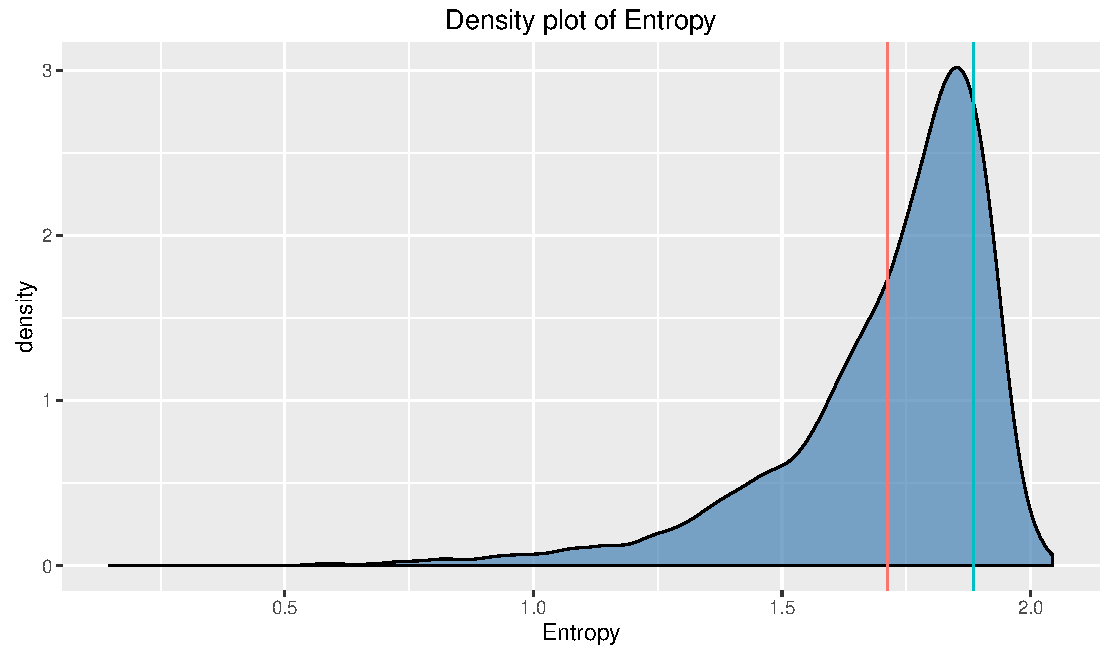
\includegraphics{Figures/Results/stabilitydens}
    \caption[Entropy density]{The plot shows the density distribution of the entropy across all nodes. The entropy of the clusters overall is shown as the red verticle line, everything to the right has less information than random.}
    \label{fig:stabilitydens}
\end{figure}


\FloatBarrier

\section{Modelling}
With the transition matrix and the bi-variate probability tables completed and tested to ensure that each table's dependencies are not random, it possible to create a forecasting model to predict day ahead portfolio load, node cluster membership and socio-demographic class. 

\subsection{Power forecasting}
The creation of a forecasting model using a transition matrix and it's comparison to a linear model baseline showed that clustering as a form of classification is an effective method for predicting day ahead domestic electricity consumption. The transition matrix was made using data from the 01-05-2011 to 15-11-2011, the test period was from 16-11-2011 to 01-01-2012.

The Transition model had an RMSE of just under 100 and a MAPE of less that 4\% this out performed the linear model which had an RMSE of 140 and a MAPE of just over 5\%, a table showing the relative performance of the two models is shown in table \ref{tab:modperf}. Figure \ref{fig:ActualVsPredLine} compares the actual to the predicted values of the model. The model tracks the actual values well but with some noise, which is most likely due to the absolute clustering caused by classifying each node into an single cluster instead of taking a more basyian probability distribution approach to cluster membership, As mentioned in figure \ref{fig:Clusterocurrance} this can result in clusters being missing on certain days and could result in artificially 'over-filling' certain clusters. The effect of missing data can be most clearly seen in the 1900 hundred cluster which is shown as a consistent outlier in \ref{fig:AbsPercErrLine} and as highly missing overall especially in the test period as shown in \ref{fig:Clusterocurrance}. 

Figures \ref{fig:resids} and \ref{fig:AbsPercErrLine} show the total error per half hour across all days and the percentage error. It can be seen that the model tends to over estimate the amount of energy in the early part of the evening until 1900 when there is an error spike of under estimation after which the bias disappears and the error varies around 0. The 1900 spike is shown in the percentage error figure to be the biggest point of error in the model when excluding outliers. The outlying day is 12-12-2011, a day with high levels of missingness that was included to ensure that the days were contiguous from the the first to the last date in the set. The missing values were imputed using the method in \ref{sec:imputation}. 
Intuitively National Holidays or days of cultural importance would have an effect on the overall domestic load. as Christmas falls in the test period it would therefore be expected that Christmas eve and Christmas day would show as outliers in the prediction model, however as figures \ref{fig:resids} and \ref{fig:AbsPercErrLine} show, these days do not in fact behave significantly differently from other days in the test period.

Figure \ref{fig:ActualVsPredErr}, is a scatter plot of half hourly predictions vs the actual load, the figure is coloured by percentage error and has the line of perfect fit shown in black. It can be seen in the figure that the model has a relatively low bias, tracking the perfect fit line well, The outlying day is shown as dark red spots above the line.

Given the low levels of error and the few strong outliers that are shown in the first 3 figures, It the density plot of the error shown in figure \ref{fig:ErrDistrib} is unsurprising. It shows a highly dense absolute error with the majority of the weight between 0\% and 5\% but that there is a long right tail indicating outliers, specifically the highly imputed 12-12-2011.

Breaking the model into half hourly performance figure \ref{fig:BoxTimeErr} shows that error across all time periods is similar with the exception of 1900 which has considerably higher than expected error as was seen in \ref{fig:resids} and \ref{fig:AbsPercErrLine}. Finally figure \ref{fig:ResidualsTime} plots a time series of the errors showing how disproportionally large the error in 12-12-2011 was, although as mentioned earlier in this section removing this day doesn't have an large effect of on the overall effectiveness of the model.

\begin{figure}
    \centering
    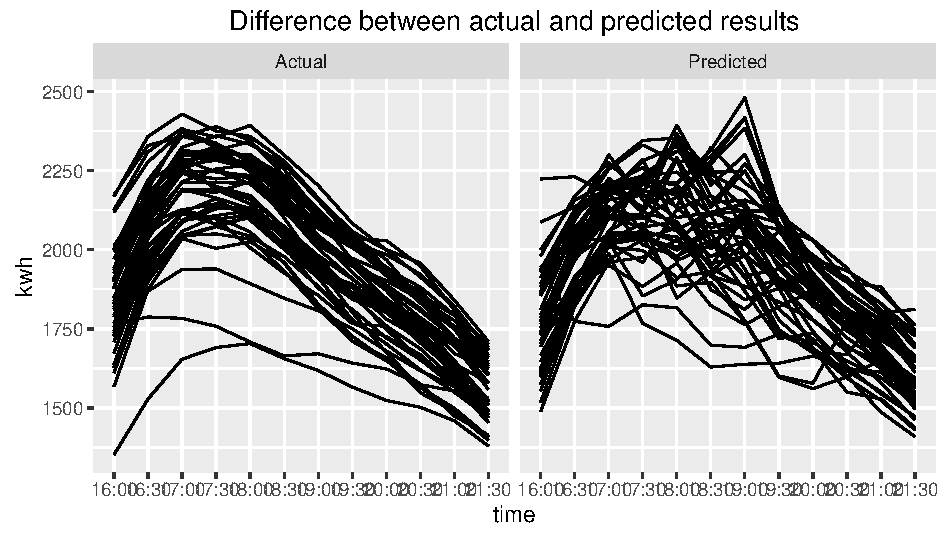
\includegraphics[width=\textwidth]{Figures/Results/ActualVsPredLine}
    \caption[Comparing actual vs predicted results]{The figure shows how the predicted values track the actual values, the general form can be seen but with noise induced. The spike of the 1900 cluster is visible as an outlier.}
    \label{fig:ActualVsPredLine}
\end{figure}

% latex table generated in R 3.3.0 by xtable 1.8-2 package
% Wed Aug 17 16:04:31 2016
\begin{table}[ht]
\centering
\begin{tabular}{rlrr}
  \hline
 & type & LinearMod & TransMod \\ 
  \hline
1 & mape & 0.05 & 0.04 \\ 
  2 & R\verb|^|2 & 0.68 & 0.84 \\ 
  3 & RMSE & 140.84 & 99.20 \\ 
   \hline
\end{tabular}
\caption{Performance metrics for the two model types} 
\label{tab:modperf}
\end{table}


\begin{figure*}[ht]
\centering
\subfloat[]{
  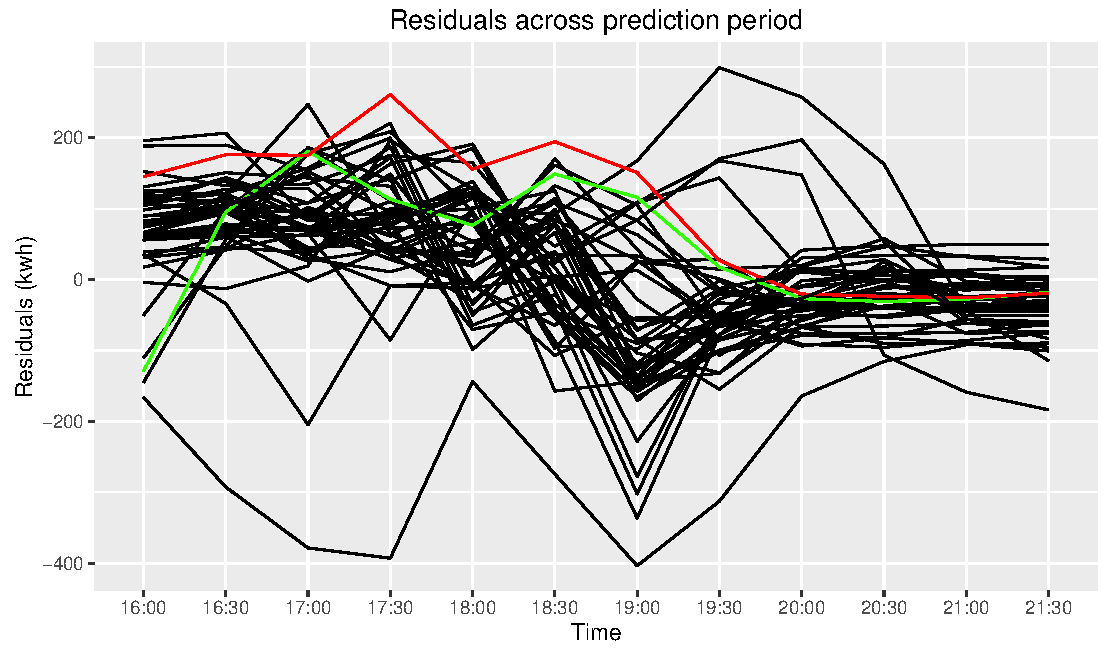
\includegraphics[width=0.49\textwidth]{Figures/Results/ResidsWXmas}\label{fig:resids}
}
\subfloat[]{
  \includegraphics[width=0.49\textwidth]{Figures/Results/AbsPercErrLine}\label{fig:AbsPercErrLine}
}

\subfloat[]{
  \includegraphics[width=0.49\textwidth]{Figures/Results/ActualVsPredErr}\label{fig:ActualVsPredErr}
}
\subfloat[]{
 \includegraphics[width=0.49\textwidth]{Figures/Results/AbsPercErrDistrib}\label{fig:ErrDistrib}
}

\subfloat[]{
  \includegraphics[width=0.49\textwidth]{Figures/Results/BoxTimeErr}\label{fig:BoxTimeErr}
}
\subfloat[]{
 \includegraphics[width=0.49\textwidth]{Figures/Results/ResidualsTime}\label{fig:ResidualsTime}
}

\caption[Cluster model analysis]{Cluster model analysis. Figures  \ref{fig:resids} and \ref{fig:AbsPercErrLine} compare error and percentage error, the synthesised day 12-12-2011 is clearly visible as the blue outlier, Christmas eve and day, are shown in green and red respectively, and are not outliers despite what intuition might suggest. The scatter plot shown in figure \ref{fig:ActualVsPredErr}, visualises the error relative to a perfect fit shown as a black line. Figure \ref{fig:ErrDistrib} shows the right skewed error distribution caused primarily by the synthesised day 12-12-2011. The higher than average prediction error at 1900 seen in \ref{fig:AbsPercErrLine}, is reflect in in figure \ref{fig:BoxTimeErr}. Finally figure \ref{fig:ResidualsTime}, shows the daily total residual level across time, with the synthesised day a clear outlier.}
\label{fig:modanalysis}
\end{figure*}

\FloatBarrier

\subsection{Node cluster forecasting}
\label{sec:NodeClustforce}
As different clusters appeared on different days, only day pairs that had the same cluster set were used for testing the node cluster foreacasting, of which there were \hl{XXX} day pairs \hl{See table XXX, in the appendix for the days}. The results of the node clustering model indicated that the transition method is not effective for predicting the movement of individual nodes. The model returned and accuracy of 0.2627, or just over 1 in 4, across the 8 different clusters. However the $\kappa$ value was 0.1121 indicating that it was effectively random, in addition the p-value was 1, strongly suggesting the predictive power is nothing as a classifier. There is several reasons that the model results can be so poor, 1 is that the classifier will mark as fail, classifying into any adjacent cluster. Even though the clusters are temporally close because they are modelled as categorical values the closeness is irrelevant. A second complicating factor is that the two most probable clusters are 1630 and 2000, which are at opposite ends of the evening this means that small differences in percentage probability can mean large swings in cluster placement. 

As a comparison the model was compared to the XGboost algorithm this model had an accuracy of 0.3644 and a $\kappa$ of 0.1739 which is still low but considerably better than the transition model. The Xgboost model with the previous 7 days clusters had a slight improvement on the simple Xgboost model with an accuracy of 0.3689 and a $\kappa$ of 0.178, both of the XGboost models had a significant p-value, which the transition matrix method does not. The recent history provided by to the XGboost model gives it a large advantage, as if there is a pattern in moving between the nodes, the XGboost model would be able to pick it up where as the transition matrix would not. Overall the poor performance of both models suggests that the behaviour of the nodes as classified by the smart meters is very noisy, this is probably a combination of the low levels of consistent behaviour that were described in \ref{sec:basicconsum} and the hard classification of the clustering algorithm. However it does suggest that there will not be problems using a transition matrix generated from a different season than the predictions as there is no clear movement between clusters that could be affected by seasonal differences. 

A comparison of the Transition model and the XGboost model with 7 days cluster movement can be seen in \ref{fig:NodeClustFore}. The figure shows the relative accuracy of the two models. A perfect predictor woud have only the diagonal in red and everything else blue. The vertical bars exhibited by both models shows that they tend to miss-classify into the 1630 and 2000 classes, however the XGboost model has a much stronger diagonal which is reflects it's higher accuracy and $\kappa$ score.


\begin{figure*}[ht]
\centering
\subfloat[]{
  \includegraphics[width=0.49\textwidth]{Figures/Results/Transitionresults}\label{fig:NodeClustTrans}
}
\subfloat[]{
  \includegraphics[width=0.49\textwidth]{Figures/Results/XGboostresults}\label{fig:NodeCLustXG}
}

\caption[Node Cluster Forecasting]{Visualising the accuracy of the Cluster transition matrix method and the XGboost method, it is clear that the XG boost method is more accurate with a much stronger diagonal than the cluster transition figure. Both clusters have higher errors on the 1630 and 2000 clusters this is likely simply because neither model is very accurate and so miss-classification ends up in these two clusters simply due to their relative size.}
\label{fig:NodeClustFore}
\end{figure*}

\subsection{Socio demographic detection}

The results of using XGboost to predict socio-demographic group based on probability of being in any given cluster did not perform any better than chance.  The accuracy of the overall model is 0.1665 and it had a $\kappa$ score close to zero,  the balanced accuracies of the individual classes was essentially 0.5 for every class. A major problem with the socio demographic detection is that the labels come from the mosaic cross classification system, where the classes of each area are based on demographic data for that area, as a result it can be noisy, making class detection difficult. In addition although there is some evidence that different social groups use energy in different ways, trying to detect it from such a small amount of data at the same time as using the experimental clustering technique may introduce too much noise to detect any signal that is actually there.

\section{Summary}

In this chapter the results of implementing chapter \ref{Method} are shown. Various decisions are made about the parameters of the analysis based on exploring the data, this includes having a minimum correlation requirement of 70\% for an edge in the graph and choosing the Louvain algorithm for clustering. In the 246 day time period, 8 clusters are detected including the Soup node, the clusters are primarily defined by the time of the mean peak of the cluster, the clusters discovered are 1630, 1700, 1730, 1800, 1830, 1900, 2000, and the node Soup. The predictive transition algorithm has a MAPE of 3.9\% which puts it on a par with other models seen in the literature and beats the linear predictor which had a MAPE of 5\%. Figures \ref{fig:ActualVsPredLine} and \ref{fig:ResidualsTime} showed that errors were induced when missing data was imputed, either in the form of raw data or clusters

The classification models that predicting the cluster of a node 1 day ahead were not as successful.The transition model had an accuracy of 25\% but a kappa score of 0.111 suggesting that it was not an effective model in comparison the XGboost models had all around better performance, the expanded XGboost model had an accuracy of 0.3689 and had a higher (but still low) $\kappa$ of 0.178, the results of these models suggest that there is a lot of noise in predicting day ahead nodes for individual smart meters. However the noisiness also suggests that using a transition matrix built with data from another season will not be a problem as if there is no pattern of movement between clusters at all there inherently cannot be any difference between seasons, therefore the transition matrix build time will not affect the results. The Socio-demographic detection was no better than random, this is likely to be due to noise in the MOSAIC classification and that socio-demographic class may not be a strong indicator of electricity consumption behaviour.







\chapter{Discussion and Conclusions}
\label{conclusions}

This chapter concludes the work done in the project by answering the research questions set in chapter \ref{Intro}, and interpreting  what it means for the electricity industry and consumers. The limitations of the study are also discussed and to what degree it is believed they have affected the results. The whole project is then concluded with some final thoughts and further work is proposed to mitigate some of the limitations or provide more insight into this type of forecasting.

\section{Interpreting the results with regards the research questions}

This project sought to answer the following 4 questions on evening peak electricity consumption.
\begin{enumerate}
\itemsep0em 
    \item Given a weighted graph of evening peak electricity consumption where the adjacency matrix is formed by a minimum correlation requirement and the distance is also a function of correlation. Does unsupervised clustering discover a meaningful set of clusters that represent electricity consumption behaviours across all days in the data set?
    
    \item Can the probability distribution produced by the graph be used to create accurate day ahead electrical load forecasts when compared to a linear model?
    
    \item It is intuitive to assume that people follow relatively consistent behaviours, for example come home from work and eat dinner at the same time each weekday. If there is consistent behaviour, membership of clusters would be relatively stable. How consistent is cluster membership? Is change between clusters non random? Can day ahead cluster membership be predicted?

    \item Does probability of cluster membership provide any insight into Socio-Demographic group?
\end{enumerate}

These questions were answered using the TC1a data set from the Customer Led Network Revolution. The data set required extensive cleaning and data munging in order to have high enough quality to perform the analysis necessary to answer the research questions. Once cleaned the data used for the analyse was the period from \hl{XXX} to 01-01-2012 covering a total of 246 days and using 5260 smart meters.  
In chapter \ref{Results} the cleaned data was developed in to a collection of weighted graphs each representing a single day in the period under analysis. In these graphs each node was a smart meter, edges were present if the Spearmans correlation was higher than 0.7 and the edge weight was proportional to the Spearmans correlation. 

The following paragraphs will describe how each research question was answered and what the answer means in terms of providing insight for companies or value for consumers

\subsection{Does unsupervised clustering provide results that have meaningful interpretation?}
The results of section \ref{sec:labelling} showed that using unsupervised clustering does provide meaningful results. Using the Louvain clustering algorithm 8 cluster families were detected including the the Soup. The 7 non-Soup clusters were defined by there peaking point giving the following cluster types,  1630, 1700, 1730, 1800, 1830, 1900, 2000, and the Soup. The 1630 and 2000 clusters were multi-modal whilst all the other clusters had a single peak. Across all clusters except the Soup the mean kWh consumed when not at peak was very low. A comparison using the walktrap clustering algorithm returned similar results but with 10 clusters instead of 8. The results show that unsupervised clustering does, discover stable cluster types across time that can be meaningfully interpretex, but that the clusters that are discovered are affected by the algorithm used.


\subsection{Can the probability distribution of the clusters be used to forecast day ahead electrical load?}
The results indicate that the probability distribution of clusters can be used to forecast day ahead electrical load. The transition matrix method out performed the linear model, with a MAPE of 3.9\% compared to a MAPE of just over 5\%. This level of performance is comparable to results found in the literature discussed in section \ref{sec:forcesmart}. The results suggest power companies can reduce their exposure to the day ahead market by using data from smart meters to reduce forecasting uncertainty. This has benefits to the grid, by reducing grid instability, the power company and consumer by reducing  reliance on volatile spot market prices and to the environment by reducing the requirement for spinning reserve and back-up generation to cover for extra load. 

The errors that the model produced, provide insight into the challenges that are faced in order to industrialise the process efficiently. The model had an error spike on the 12-12-2011 a day when there was very little information provided by the smart meters due to some kind of data collection error, shown in figure
\ref{fig:ResidualsTime}. This error should be considered in the context of the amount of cleaning required to make the data workable (chapter \ref{DataCleaning}). It shows the need for reliable data supplies in order to build and deploy statistical models based on distributed data sources. The other main error produced by the model was in the 1900 cluster as shown in figure \ref{fig:ActualVsPredLine}. This error was caused by the modelling process itself. The clustering method used non-overlapping clusters, resulting in some clusters being only intermittently present (see figure \ref{fig:Clusterocurrance}). The error occurred because the Bayesian approach to node membership prediction which always proposed all clusters, clashed with the hard clustering method which didn't. In winter, the period of the test set, the 1900 cluster was only intermittently present. This meant that the mean cluster profile used to predict the load was out of date, in cases where the weather was considerably different this would cause prediction errors, as shown in figure \ref{fig:BoxTimeErr}.

\subsection{Can cluster membership be predicted?}

The transition model for predicting movement between clusters was not a reliable method of predicting next day transitions. The model had an accuracy of 0.2627 and a $\kappa$ score of 0.1121 indicating that the results were no better than chance, this view was also supported by the p-value of 1 indicating that the model is not predictive. The two XGboost models performed similarly to each other and slightly better than the transition model. The Expanded XGboost model had the best results with an accuracy of 0.3644 and a $\kappa$ of 0.1739. Whilst not a strong performer the XGboost models were definitely better than the transition method. In many ways it is not surprising that the model was not very predictive when considering the analysis of self correlation in figure \ref{fig:MeanAbsCorr}. The figure showed that on average the absolute correlation of a smart meter with itself across multiple days was only 0.3. The low levels of correlation and the difficulty in predicting movement from cluster to cluster is most likely influenced by domestic energy consumption being only 20\% electricity, which is small compared to gas which makes up 60\%. In addition the prediction was compounded by the non-overlapping clustering technique, as mentioned in \ref{sec:NodeClustforce} there were only \hl{XXX} day pairs that had the same clusters. The non-overlapping nature of the clusters meant that borderline cases were perhaps arbitrarily assigned to a cluster depending on how other smart meters had behaved. Being able to predict next day clustering allows the company to send direct messages to consumers advising about high charges providing benefit to both the supplier and the consumer.

\subsection{Can socio-demographic class be inferred from cluster information}
The results of using an XGboost to predict Mosaic class membership did not perform any better that random. Despite using all cluster transitions for the whole 246 days, the model failed on every metric obtaining a $\kappa$ score of almost zero and failing to provide any meaningful predictions in any of the 16 classes. 

One problem may be that Mosaic infers the socio-demographic class of an area based on data available on that area. This means that households have been classified using an area's  socio-demographic group may not belong in that group but another. However the complete failure of the model to find any pattern suggests that, in this form, clusters are not a useful way to infer consumer socio-demographic groups. A reason for this is that certain peaks may be cross cultural, such a lot of people finish work at 5pm, popular television is on at the same time across all channels and genres, children all finish school at 1530 and so on. These general societal patterns combined with the noise in the Mosaic data can combine to mask any signal that could be present. 

More broadly the use of socio-economic data to make customer inferences should be treated with care. Studies have shown that there is scepticism amongst the public of what companies can find out about them through smart meters \cite{buchanan2016}, and the public may not be positive about companies studying their family life and levels of wealth. However as a major benefit of smart meters is to support fuel poor households \cite{clastres2016}, it is possible that this could be classed as "legitimate business application" as discussed by Mckenna et al \cite{mckenna2012}. The three way balance between, the economic possibilities of more customer insight, the ability to protect vulnerable households, and customers rights to privacy will become an increasingly important issue as technology improves, especially with the ability to disaggregate load to appliance level \cite{kavousian2013} \cite{weiss}.


\section{Limitations}
\begin{itemize}
    \item \textbf{Geography}: No geographic analysis was performed in this project. As all the data comes from the same part of the north of England it was assumed that the weather patterns and climate would be similar across all homes. There may however be differences especially between coastal and inland residential areas. If the node to cluster prediction model had been strong and the cluster transition model weaker that would have suggested that geography could have an influence on results . However as there were no strong results for individual nodes to cluster prediction and strong results for overall load prediction, it suggests that geography is not an issue.

    \item \textbf{Non-overlapping clusters}: As has been seen throughout this work combining hard clustering techniques with a Bayesian approach to forecasting creates conflicts in prediction results. Although this wasn't a serious issue for load forecasting it was with day ahead cluster membership prediction. Using a soft-clustering approach may provide a more informative view of which cluster nodes will be in the following day.

    \item \textbf{Evening only}: The data only explores the evening peak, this provides several difficulties. With half hourly data there are only 12 time periods with which to calculate the correlation, this is not long enough to check to see if the results were statistically significant as was done by  Mantegna \cite{mantegna1999}, however even if some of the correlations are spurious the consistent results indicate that on aggregate correlating on so few examples was not a problem. 
    
    A second issue with using only the evening peak is that it provides no knowledge or insight into the rest of the day or even demonstrates full day applicability. However as the evening peak is of such importance, for suppliers, and contains such large variance, a focus on the evening peak provides the best opportunity to test the model on the part of the day that is most taxing to power companies. It also should be considered that if the number of periods was increased this may have a dramatic effect on the number of clusters as many more behavioural types emerge. A full day solution may be to break the day into chunks, for example, morning rush, day time, evening peak, night. and create behaviours for the distinct day-cycle phases.

    \item \textbf{Out of season transmission matrix}: The transmission matrix was made using data from summer and autumn and used to predict results in winter, which could be problematic as electricity is consumed differently at different times of year. The interesting detail with this prediction method is that only the the node movements are predicted directly not the actual load. This means that unless the patterns of inter cluster movement change from summer to winter, not just the magnitude of consumption, the model will work well. The poor performance of the node cluster prediction model compared to the good performance of the transition load model indicates that this isn't a limitation. If clusters could be predicted with accuracy it would indicate a clear pattern of movement, and thus the possibility that this pattern is also linked to the seasons. However as this is not the case there can also not be any seasonality issues.
    
    \item \textbf{Predefined clusters}: As was mentioned in chapter \ref{Method} the transmission matrix is created using clusters from the whole data set and not just the number of days that have occurred. This means that although the matrix doesn't directly include data from the future the definition of a cluster family is informed by events that have not yet happened. It also raises the issue that new clusters could emerge, if for example there were a full years data. Resolving this issue depends a lot on forecast strategy. Recalculating the transmission matrix everyday to take into new account new information is one method, alternatively the transmission matrix could be built and then set so as not to change. Whilst this limitation doesn't invalidate the results it could be considered bad practice.
    
    \end{itemize}


\section{Conclusion}

The combination of the load profile prediction, the cluster membership prediction and the socio-demographic detection all tie together with the UK government's vision of a low carbon smart grid. By using the data from the smart meters to create accurate load forecasts for day ahead prediction, benefit can be provided to the consumer, supplier and environment. These benefits come from reducing exposure to volatile spot markets, and the requirement to have expensive back up generation online. Although possibly a controversial invasion of privacy the socio-demographic detection of fuel poor households enables the results of the smart meter cluster membership model to identify when consumers are likely to use energy at peak times, this allows the supplier to intervene directly by for example sending a targeted text message or email to the customer suggesting that they use large appliances later or earlier in the day. 

Unfortunately this vision of the future of smart grids where control remains with the consumer is still some way off. Although the load prediction model was successful the smart meter cluster membership did not perform strongly and the socio-demographic detection model did not work at all. 

Some of the problems can be accounted for by data quality issues with the TC1a dataset and the Mosaic socio-demographic labelling system, however other problems are clearly an inherent part of the technique. Most of the problems are related to using a non-overlapping clustering method which leads to clusters not being present on some days and so inducing errors (Cluster 1900 is a good example figures \ref{fig:BoxTimeErr} and \ref{fig:Clusterocurrance}).

In conclusion the use of graph based prediction methods for day ahead load forecasting is an effective tool, that tells the supplier not only how much energy is going to be consumed the following day but also in what way it will be consumed. With some additional work, vulnerable consumers can be provided with support on when to use energy and consumers overall can be provided with a way of making informed decisions on fuel use without surrendering control of household appliances to the electricity supplier. Such a technique is a valuable tool in creating a flexible smart grid for a low carbon future.


\section{Contributions}
The main contributions of the work are as follows
\begin{itemize}
\itemsep0em 
    \item Demonstrating that behavioral patterns can be uncovered using unsupervised clustering on a graph.
    \item A novel forecasting approach using the probability of transmission between behavioural clusters.
    \item A Cleaned model of the CLNR TCa1 data set that is ready for data mining with minimal further processing. This dataset will be presented to \href{http://www.nature.com/sdata/about}{Nature: Scientific Data} for publication later in the year.
    \item A set of functions in R which allow for the visualisation of the structure of large matrices as hierarchically structured heatmaps.
\end{itemize}


\begin{itemize}
    \item The the transition matrix is made using clusters that have been defined using data that has occurred after the time period of the transition matrix. The assumption is that the number of clusters stabilises with a high enough day count, but this might not be the case. by finding cluster families using distinct time horizons and comparing the make up of those families it would then be clear whether using a static transition matrix is appropriate or whether the family clustering and transition matrix has to be recalculated everyday in order to provide reasonable predictive results
    
    \item Using non-overlapping clusters causes several interesting artifacts, such as missing clusters on certain days and very clearly defined cluster profiles. What effect does using overlapping clusters have on the relative size of the clusters each day and how does the load profile of each cluster differ from the load profiles of the non-overlapping case.
    
    \item How does the model performance change when a larger part of the energy mix is included such as gas, or comparing with a country where a larger percentage of household energy is electricity such as Norway.

    \item The low levels of electricity use means that there is high volatility, performing the same analysis again but using volatility as the graph edge metric, would maybe help stratify consumers into low and high levels of predictability which would be useful for hedging strategies.
    
    \item The Cluster Transition matrix was created using all 5260 nodes, however similar to the findings of \cite{kavousian2013} on a large network it may provide diminishing returns to use increasingly large amounts of nodes. Likewise the number of days required for the transition matrix to converge to stability is also unknown. It would be useful to map the parameter space of node number and time horizon required to create a transition matrix that had a KL divergence of zero. Having this knowledge would allow Energy companies to reduce the amount of bandwidth taken up by smart meter data transfer whilst maintaining the same forecasting ability.
    
    \item Due to the cyclical nature of electricity consumption (see Literature review \ref{lit:load}) the transition matrix can also be split by day of the week, this would make the transition matrix larger but may give more accurate results capturing within week transition probabilities. An exploration of how clusters should be defined, e.g day to day, weekday to weekend, day of the week, etc, could give a better understanding of how to optimise the transition matrix for accuracy.
\end{itemize}
\addcontentsline{toc}{chapter}{Appendices}

% The \appendix command resets the chapter counter, and changes the chapter numbering scheme to capital letters.
%\chapter{Appendices}
\appendix
\chapter{Plotppendix}
\label{Plotpend}
This appendix hold the additional plots and tables that provide contextual information useful but not essential for understanding the project.  


\section{Additional plots}

\begin{figure}
    \centering
    \includegraphics[width = \textwidth]{Figures/Appendix/logenergydensity}
    \caption[Log energy density]{The $log_{10}$ plot of the density shown in Figure \ref{fig:energydensity}. It can be seen that the distribution of this data is approximately normal in log space.}
    \label{fig:logenergydensity}
\end{figure}


\begin{figure}
    \centering
    \includegraphics[width = \textwidth]{Figures/Appendix/AllNodesClustercolour}
    \caption[All Nodes for one day]{The distinct cluster forms can be seen across all the clusters, the soup node has no pattern and is clearly just noise.}
    \label{fig:AllNodesClustercolour}
\end{figure}


\begin{figure}
    \centering
    \includegraphics[width = \textwidth]{Figures/Appendix/AllCLustFamilies}
    \caption[All Clusters grouped by family]{The distinct cluster forms can be seen across all the clusters, the soup node has no pattern and is clearly just noise.}
    \label{fig:AllCLustFamilies}
\end{figure}

\FloatBarrier

\section{Additional tables}
% latex table generated in R 3.3.0 by xtable 1.8-2 package
% Wed Aug 17 16:25:24 2016
\begin{table}[ht]
\centering
\begin{tabular}{rlrrrrrrrr}
  \hline
 & ClustID & 1630 & 1700 & 1730 & 1800 & 1830 & 1900 & 2000 & soup \\ 
  \hline
1 & 1630 & 0.31 & 0.13 & 0.09 & 0.09 & 0.08 & 0.06 & 0.22 & 0.01 \\ 
  2 & 1700 & 0.23 & 0.17 & 0.12 & 0.11 & 0.08 & 0.06 & 0.22 & 0.01 \\ 
  3 & 1730 & 0.18 & 0.13 & 0.16 & 0.13 & 0.10 & 0.06 & 0.23 & 0.01 \\ 
  4 & 1800 & 0.16 & 0.11 & 0.13 & 0.16 & 0.12 & 0.07 & 0.24 & 0.01 \\ 
  5 & 1830 & 0.16 & 0.09 & 0.10 & 0.13 & 0.14 & 0.09 & 0.28 & 0.01 \\ 
  6 & 1900 & 0.16 & 0.09 & 0.09 & 0.10 & 0.13 & 0.12 & 0.31 & 0.01 \\ 
  7 & 2000 & 0.15 & 0.09 & 0.08 & 0.09 & 0.10 & 0.08 & 0.40 & 0.01 \\ 
  8 & soup & 0.20 & 0.09 & 0.08 & 0.10 & 0.09 & 0.06 & 0.24 & 0.14 \\ 
   \hline
\end{tabular}
\caption{The cluster transition probabilities} 
\label{tab:clustrans}
\end{table}

% latex table generated in R 3.3.0 by xtable 1.8-2 package
% Thu Sep  1 11:38:29 2016
\begin{longtable}{rll}
  \hline
 & First.Pair & Matching.Pair \\ 
  \hline
1 & 2011-05-17 & 2011-05-18 \\ 
  2 & 2011-05-18 & 2011-05-19 \\ 
  3 & 2011-05-22 & 2011-05-23 \\ 
  4 & 2011-05-24 & 2011-05-25 \\ 
  5 & 2011-05-25 & 2011-05-26 \\ 
  6 & 2011-05-26 & 2011-05-27 \\ 
  7 & 2011-05-27 & 2011-05-28 \\ 
  8 & 2011-06-02 & 2011-06-03 \\ 
  9 & 2011-06-05 & 2011-06-06 \\ 
  10 & 2011-06-12 & 2011-06-13 \\ 
  11 & 2011-06-13 & 2011-06-14 \\ 
  12 & 2011-06-19 & 2011-06-20 \\ 
  13 & 2011-06-20 & 2011-06-21 \\ 
  14 & 2011-06-22 & 2011-06-23 \\ 
  15 & 2011-06-23 & 2011-06-24 \\ 
  16 & 2011-06-25 & 2011-06-26 \\ 
  17 & 2011-06-30 & 2011-07-01 \\ 
  18 & 2011-07-02 & 2011-07-03 \\ 
  19 & 2011-07-03 & 2011-07-04 \\ 
  20 & 2011-07-04 & 2011-07-05 \\ 
  21 & 2011-07-05 & 2011-07-06 \\ 
  22 & 2011-07-06 & 2011-07-07 \\ 
  23 & 2011-07-09 & 2011-07-10 \\ 
  24 & 2011-07-10 & 2011-07-11 \\ 
  25 & 2011-07-11 & 2011-07-12 \\ 
  26 & 2011-07-13 & 2011-07-14 \\ 
  27 & 2011-07-14 & 2011-07-15 \\ 
  28 & 2011-07-18 & 2011-07-19 \\ 
  29 & 2011-07-24 & 2011-07-25 \\ 
  30 & 2011-07-26 & 2011-07-27 \\ 
  31 & 2011-07-27 & 2011-07-28 \\ 
  32 & 2011-07-28 & 2011-07-29 \\ 
  33 & 2011-07-29 & 2011-07-30 \\ 
  34 & 2011-08-11 & 2011-08-12 \\ 
  35 & 2011-08-12 & 2011-08-13 \\ 
  36 & 2011-08-14 & 2011-08-15 \\ 
  37 & 2011-08-16 & 2011-08-17 \\ 
  38 & 2011-08-17 & 2011-08-18 \\ 
  39 & 2011-08-19 & 2011-08-20 \\ 
  40 & 2011-08-25 & 2011-08-26 \\ 
  41 & 2011-09-01 & 2011-09-02 \\ 
  42 & 2011-09-05 & 2011-09-06 \\ 
  43 & 2011-09-08 & 2011-09-09 \\ 
  44 & 2011-09-09 & 2011-09-10 \\ 
  45 & 2011-09-23 & 2011-09-24 \\ 
  46 & 2011-09-28 & 2011-09-29 \\ 
  47 & 2011-10-03 & 2011-10-04 \\ 
  48 & 2011-10-04 & 2011-10-05 \\ 
  49 & 2011-10-08 & 2011-10-09 \\ 
  50 & 2011-10-09 & 2011-10-10 \\ 
  51 & 2011-10-16 & 2011-10-17 \\ 
  52 & 2011-10-17 & 2011-10-18 \\ 
  53 & 2011-10-18 & 2011-10-19 \\ 
  54 & 2011-10-19 & 2011-10-20 \\ 
  55 & 2011-10-23 & 2011-10-24 \\ 
  56 & 2011-10-28 & 2011-10-29 \\ 
  57 & 2011-11-01 & 2011-11-02 \\ 
  58 & 2011-11-06 & 2011-11-07 \\ 
  59 & 2011-11-09 & 2011-11-10 \\ 
  60 & 2011-11-16 & 2011-11-17 \\ 
  61 & 2011-11-17 & 2011-11-18 \\ 
  62 & 2011-11-25 & 2011-11-26 \\ 
  63 & 2011-12-02 & 2011-12-03 \\ 
  64 & 2011-12-07 & 2011-12-08 \\ 
  65 & 2011-12-15 & 2011-12-16 \\ 
  66 & 2011-12-26 & 2011-12-27 \\ 
   \hline
\hline
\caption{Day pairs with matching clusters} 
\label{tab:DayPairs}
\end{longtable}


\chapter{Community distance}
\label{community distance}

An interesting question to consider is the graph distance between two communities that share no common nodes. This is interesting because if two graphs share no common nodes then intuitively they shouldn't be in the same cluster of communities. Although solving this problem is beyond the scope of this project, the discussion below describes some cases and shows that probability of randomly moving from y to x decreases exponentially with a linear increase in additional connected clusters.

In this section communities will be represented as nodes which are made up of a binary vector of length l (each element representing a node in the original graph ), the edges of the graph are defined by the Jaccard similarity coefficient (JSC) betwen the node vectors. A JSC of 0 means no edge for any other value, the edge distance is the JSC and it's probability weight is the normalised inverse JSC. This  is shown in equations \ref{eq:JSC} and \ref{eq:JSCdist}. In this context the distance graph is undirected and the graph of weighted probabilities is directed.

\begin{equation}
    J(A,B)=\frac{A\cap B}{A\cup B}=JSC
    \label{eq:JSC}
\end{equation}


\begin{equation}
    \frac{1}{JSC}=\frac{A\cup B}{A\cap B}=Dist
    \label{eq:JSCdist}
\end{equation}


\section{Question 1:} When there are three nodes in the network what is the minimum distance between nodes $x$ and $y$, a schematic of this graph can be seen in \ref{net:threenodes}

\begin{figure}[ht]
    \centering
    \includestandalone{Tikz/CommDist/threenodes}
    \caption[Three Node graph]{Three node setup, showing the relationships within the network.}
    \label{net:threenodes}
\end{figure}

As it is stated that$x_1 \notin y$, then $ y\cup S \supset y $ as $S$ must have at least 1 element of $x$ as a result $K \cup S$ (K is either of the none overlapping sets) is a proper superset of both $y$ and $x$. Fully defined $K \cup S = y \cup x \cup z$ where $z$ are all elements that are not members of either $y$ or $x$, giving in total 3 non overlapping sets.

Therefore to minimise the distance from node y to S, $y \cap S$ needs to be maximised. This occurs when the entire of $y$ is found in vector $S$ making the resulting JSC between the two nodes. 

\begin{equation}
    \frac{|y|}{|x|+|y|+|z|}
\end{equation}

and the distance

\begin{equation}
    \frac{|x|+|y|+|z|}{|y|}
\end{equation}

The distance between $x$ and $y$ is then

\begin{equation}
    \frac{|x|+|y|+|z|}{|y|} +\frac{|x|+|y|+|z|}{|x|} = 2 + \frac{|z|}{|x|+|y|}+\frac{|x|^2+|y|^2}{|x||y|}
\end{equation}

Which is minimised when $z=0$ and $|x|=|y|$ making the minimum distance between two non-overlapping nodes separated by a common node 4 as shown below


\begin{equation}
    4 =2 + \cancel{\frac{0}{|x|+|x|}}+\frac{|x|^2+|x|^2}{|x||x|} =2+\frac{2\cancel{|x|^2}}{\cancel{|x|^2}}
\end{equation}


The resulting weighted graph can be seen in figure \ref{net:weight3nodes}

\begin{figure}
    \centering
    \includestandalone{Tikz/CommDist/weighted3nodes}
    \caption[Three Node directed graph]{The Weighted directional graph shows the probability of moving from 1 node to another}
    \label{net:weight3nodes}
\end{figure}

\section{Question 2:}
Building on the previous section the effect on probability of of moving from y to x is considered with more than one connecting node. What is the probability of having arrived at node x by time t or earlier given n nodes where $S=S_n$?

To begin this problem, the previous problem can be considered with two overlapping nodes (where $S_1=S=2$) instead of 1. Figure \ref{net:4nodes} shows the construction of such a graph and that the distance between the identical nodes is 1 as would be expected when using inverse Jaccard distance.


\begin{figure}[ht]
    \centering
    \includestandalone{Tikz/CommDist/fournodes}
    \caption[Four node graph]{Weighted undirected graph shows the distance between the nodes of the network when there are two identical joining nodes.}
    \label{net:4nodes}
\end{figure}



The extension of figure \ref{net:4nodes} is to increase from 2 to n identical connecting nodes. The number of edges connecting x and y to the S nodes are n each, the number of edges connecting the S nodes with each other follows the triangle number series $E=\frac{(n-1)n}{2}$. As the S nodes are all identical they can be represented as a simplified directed weighted graph as shown in figure \ref{net:Nnodesweighted}. The derivation of the weights is shown in equations \ref{eq:unormweights} to \ref{eq:stayinS}.

\begin{figure}[ht]
    \centering
    \includestandalone{Tikz/CommDist/Nnodes}
    \caption[N node unweighted Graph]{This undirected graph shows all the edges of a network of n+2 nodes where 2 two nodes have no overlap and n nodes are identical and whose make up means the distance between x and y is minimised. Distances have not been included but are similar to figure \ref{net:4nodes} in that links to the S nodes are length 2 and between S nodes are length 1}
    \label{net:Nnodes}
\end{figure}


\begin{figure}[ht]
    \centering
    \includestandalone{Tikz/CommDist/Nweighted}
    \caption[N node transfer probability]{Weighted directed graph shows the probability of transfer between nodes in the network when there are n identical joining nodes that make up the set S. There is no arrow back from x as once the random process has reached x the process halts.}
    \label{net:Nnodesweighted}
\end{figure}

The sum of unormalised weights of S are 
\begin{equation}
    \frac{2+(n-1)n}{2}= \frac{1}{2}+\frac{1}{2}+\frac{(n-1)n}{2}= 1+\frac{(n-1)n}{2}
    \label{eq:unormweights}
\end{equation}

Using this as a normalisation constant probability of transferring from S to either x or y is 
\begin{equation}
    \frac{1}{2+(n-1)n}=\frac{\frac{1}{\cancel{2}}}{\frac{2+(n-1)n}{\cancel{2}}}
\end{equation}

The normalised probability of stay in in the S is given by
\begin{equation}
        \frac{(n-1)n}{2+(n-1)n}=\frac{\frac{(n-1)n}{\cancel{2}}}{\frac{2+(n-1)n}{\cancel{2}}}
        \label{eq:stayinS}
\end{equation}


\chapter{UK domestic Energy breakdown}
\label{sec:Energybreakdown}
Breaking down the domestic energy mix of the UK \cite{domesticenergyv2pdfwithnotes2005} provides more insight into why there could be the low correlations found in \ref{sec:basicconsum}. Overall the majority of UK domestic energy comes from gas, as shown in figure \ref{fig:DomElConsumFuel}, which which makes up over 70\% of the mix compared to 20\% from electricity. Across all fuel types the majority of energy is used on Space heating and water heating which accounts for more than 80\%. When looking at only electricity consumption over 60\% of electricity is used on lighting and appliances with very little on heating. The result is that turning on lights, TV's or computers will have a major effect on consumption, even though they are small relative to the base load of energy consumption overall. This supports the finding of low levels of correlation within a smart meter a minor changes in unimportant object of electricity consumption will have a major effect on the evening behaviour pattern introducing variability.

\begin{figure}
    \centering
    \includegraphics[width =\textwidth]{Figures/Appendix/DomConsumType}
    \caption[Domestic energy consumption by end of use]{Breaking down UK domestic energy consumption by end use across all fuel types it is clear that heating (the combination of SpaceHeating and Water), is the single biggest use of energy consumping over 84\% of all domestic electricity.}
    \label{fig:DomConsumType}
\end{figure}

\begin{figure}
    \centering
    \includegraphics[width =\textwidth]{Figures/Appendix/DomElConsumType}
    \caption[Domestic electricity consumption by end of use]{Breaking down domestic electricity use by end of use shows that the single biggest use of electricity in the home is lighting and Appliances, this contrasts strongly with figures \ref{fig:DomConsumType} overall breakdown of electricity use}
    \label{fig:DomElConsumType}
\end{figure}

\begin{figure}
    \centering
    \includegraphics[width =\textwidth]{Figures/Appendix/DomElConsumFuel}
    \caption[Energy consumption by fuel type]{The breakdown of energy fuel types shows that electricity is only 20\% of the total fuel mix gas being about 70\% of total energy consumption.}
    \label{fig:DomElConsumFuel}
\end{figure}

\iffalse
\chapter{Flow Chart of Data process}
The flow charts in this section provide a visual representation of how the project was performed, figure \ref{fig:CleanFlow} shows how the data set TC1a was manipulated so that the the most high quality segments of the data were included and the remaining NA's filled. Figure \ref{fig:ProcessFlow} goes from the cleaning stage, and shows how the data is processed so that it the transition matrix and predictive model can be made and tested. The combination of both figures therefore gives a high level overview of the project from start to finish.

\begin{landscape}

\begin{figure}[ht]
    \centering
    \includegraphics[width =\textwidth]{Figures/Appendix/DataCleaning.png}
    \caption[Data cleaning process]{Flow chart of the Data Cleaning Process}
    \label{fig:CleanFlow}
\end{figure}


\begin{figure}[ht]
    \centering
    \includegraphics[width =\textwidth]{Figures/Appendix/Thesisprocess.png}
    \caption[Project process]{Flow chart showing the process of generating and testing the predictive model once the data has been cleaned}
    \label{fig:ProcessFlow}
\end{figure}


\end{landscape}
\fi

\chapter{Colophon}
\label{appendixlabel3}
This document was set in the Times Roman typeface using \LaTeX\ and Bib\TeX , composed with ShareLaTeX using the UCL thesis template developed by Ian Kirker. Template Sourcecode can be obtained either through the ShareLaTeX setup wizard or on \href{https://github.com/UCL/ucl-latex-thesis-templates/blob/master/Main.tex}{UCL's Github account}.
The compilable script for this full thesis can be found at \href{https://github.com/JonnoB/MscDissertation}{MscDissertation}. For sharpness, images were imported as PDF files, or if that was not possible as PNG's. All figures were made using R's ggplot2 package, graphs were visualised using either igraph \cite{csrdi2006} or Gephi \cite{bastian2006}.
 % description of document, e.g. type faces, TeX used, TeXmaker, packages and things used for figures. Like a computational details section.
% e.g. http://tex.stackexchange.com/questions/63468/what-is-best-way-to-mention-that-a-document-has-been-typeset-with-tex#63503

% Side note:
%http://tex.stackexchange.com/questions/1319/showcase-of-beautiful-typography-done-in-tex-friends

\chapter{Computational Details}
\label{TechComp}

Computation was performed using cloud computing was performed on amazon EC2 instance. 
The specifications of the instance was scaled according to computational requirements of the specific operation being performed but mostly using the instance shown in table \ref{tab:Machspec}. The image used on the EC2 was obtained from the website of \href{http://www.louisaslett.com/RStudio_AMI/}{Louis Aslett}. All calculations were performed using \href{https://www.r-project.org/}{R} version ' Bug in Your Hair' (3.3.1)  \cite{rcoreteam2016}. Packages used can be seen in section \ref{sec:packages}. Gephi version 0.9.1 was used for graph visualisation. Source code was managed using Github through Github windows desktop application version "Oh Darth, Where Art Thou?" (3.1.1.4), For reproducibility the code for this project can be found at \href{https://github.com/JonnoB/SmartMeterThesisCode}{SmartMeterThesisCode}.

\begin{table}[h]
\centering
\begin{tabular}{|l|l|}
\hline
Machine   & M4 Extra Large            \\ \hline
OS        & Ubuntu 16.04.1               \\ \hline
Processor & 2.4 GHz Haswell processors \\ \hline
RAM       & 16Gb                      \\ \hline
\end{tabular}
\caption{Machine Specifications}
\label{tab:Machspec}
\end{table}

\begin{figure}
    \centering
    \includegraphics[width = \textwidth]{Figures/Appendix/SoftwareType}
    \caption[Software used]{Breakdown of the time used on each software type in this project.}
    \label{fig:SofwareType}
\end{figure}


\section{R Packages}
\label{sec:packages}
The Following R packages were used in this project

stringr \cite{wickham2015}, lubridate \cite{grolemund2011}, data.table \cite{dowle2015}, caret \cite{fromjedwing2016}, xgboost \cite{chen2016}, e1071 \cite{meyer2015}, R.utils \cite{bengtsson2016}, Hmisc \cite{harrelljr2016}, Matrix \cite{bates2016}, ff \cite{adler2014}, zoo \cite{zeileis2005}, networkD3 \cite{gandrud2016}, igraph \cite{csardi2006} \cite{csrdi2006}, magrittr \cite{bache2014}, ggplot2 \cite{wickham2009}, tidyr \cite{wickham2016}, xtable \cite{dahl2016}, entropy \cite{hausser2014}, dplyr \cite{wickham2016a}, microbenchmark \cite{mersmann2015}.


 
% You could separate these out into different files if you have
%  particularly large appendices.

% This line manually adds the Bibliography to the table of contents.
% The fact that \include is the last thing before this ensures that it
% is on a clear page, and adding it like this means that it doesn't
% get a chapter or appendix number.
\addcontentsline{toc}{chapter}{Bibliography}

% Actually generates your bibliography.
\printbibliography

% All done. \o/
\end{document}
